%-----------------------------------------------------------------------------
%	PACKAGES AND DOCUMENT CONFIGURATION
%-----------------------------------------------------------------------------

% Use `report` class with `USCthesis` package (style file) by Brian P. Gerkey
\documentclass{report}
% [options] can be any of these default/alternative flag:
%   dissertation/thesis, final/proposal, copyright/nocopyright,
%   fussy/sloppy, flushbottom/raggedbottom, clref/opref.
\usepackage[proposal]{USCthesis}

% Packages required by `USCthesis.sty`.
\usepackage{setspace}
\usepackage{tabularx}
% Filler text for formatting. Comment these lines out for real writing.
\usepackage[english]{babel}
\usepackage{blindtext}
\usepackage{indentfirst, times, graphicx, subfigure, natbib, mathtools, setspace, amsmath, multirow, algorithm, epstopdf, amsmath, amsthm,
  amssymb, algorithmic}
\newtheorem{theorem}{Theorem}
\newtheorem{remark}{Remark}
\newtheorem{lemma}{Lemma}
\newtheorem{definition}{Definition}
\newtheorem{example}{Example}

\newtheorem{proposition}{Proposition}
\newtheorem{corollary}{Corollary}
\begin{document}

%-----------------------------------------------------------------------------
%	TITLE PAGE
%-----------------------------------------------------------------------------

% Volume name could be added as option, e.g. `[Volume I]`.
\title{Theoretical and Computational Foundations for Cyber-Physical Systems Design}

\author{Yuankun Xue}

% Committee list is only shown in `proposal` layout.
\committee{Professor Paul Bogdan & (Chair)\\
           Professor Peter A. Beerel\\
           Professor Edmond A. Jonckheere \\ 
           Professor Bhaskar Krishnamachari\\
           Professor Aiichiro Nakano
           }

% Submission information is only shown in `final` layout.
\majorfield{Electrical Engineering}
\submitdate{April 2017}

%-----------------------------------------------------------------------------
%	PREFACE
%-----------------------------------------------------------------------------

% The preface environment prints the title page.
\begin{preface}

  % Dedication Page, which is truly unnecessary.
  %\prefacesection{Dedication}
  %  This dissertation is dedicated . . .
  %   \begin{quote}
  %       \raggedleft {\em To x, y}\\
  %       \raggedleft {\em and especially to z.}
  %   \end{quote}

  % Acknowledgement Page, which is also unnecessary for proposals.
  %\prefacesection{Acknowledgements}
    % Better to separate LaTeX structure and content
  %  The author acknowledges the partial financial support of ...

I would like to thank my advisor ...

I would like to thank my committee members ...

I would like to thank all of my friends ...

Finally, I would like to thank my family ...


  \tableofcontents
  \listoftables
  \listoffigures

  % Abstract Page
  \prefacesection{Abstract}
    Recent astonishing advances on cognitive sensing modalities, data science, machine learning frameworks, communication and computation design methodologies not only enable us to capture, analyze and impact such multi-system interactions with remarkably improved accessibility, operability, resolution and sophisticated mathematical and processing frameworks, but also calls for a radically novel integration of state-of-art techniques in both \textit{theoretical} and \textit{computational} domains to endow the cyber-physical systems (CPS) with built-in \textit{intelligence} and realtime processing capabilities. The  intelligent CPS is prescribed by the urgent demands for a revolutionary shift from the manually intervened analyzing paradigms to a self-aware, self-optimized and self-configured systems of extreme autonomy to facilitate adaptive sensing (i.e., data collection), learning (i.e., data processing) and decision making (i.e., control) processes with minimal human supervision over extended periods of operation. However, porting the embedded intelligence to devices with strict real-time processing constraints raises concerns with respect to the applicability of the well-established general-purpose computing paradigms (e.g., CPU/GPU array or clusters, data centers, cloud-computing) to application scenarios that have i) exorbitantly large amount of raw data, ii) limited  or insufficient communication bandwidth and/or iii) strict power,  thermal budget and timing constraints. These objectives can not be reached without an integrated mathematical and computational framework that is able to  i) capture and understand the complex interdependent structure of CPS processes rich in stochasticity and ii) provides real-time processing capabilities that can be encompassed by on-board computing powers dynamically optimized for interested CPS applications. \\
\indent In this proposal, we aim to address these challenges by embracing the novel mathematical framework in modeling and control theory and advocating for a top-down design methodology for computing and communication platforms. We propose a new mathematical strategy for constructing compact yet accurate models of complex systems dynamics that aim to scrutinize the causal effects and influences by analyzing the statistics of the magnitude increments and the inter-event times of stochastic processes. We derive a framework that enables to incorporate knowledge about the causal dynamics of the magnitude increments and the inter-event times of stochastic processes into a multi-fractional order nonlinear partial differential equation for the probability to find the system in a specific state at one time. Rather than following the current trends in nonlinear system modeling which postulate specific mathematical expressions, this mathematical framework enables us to connect the microscopic dependencies between the magnitude increments and the inter-event times of one stochastic process to other processes and justify the degree of nonlinearity. In addition, the proposed formalism allows to investigate appropriateness of using multi-fractional order dynamical models for various complex system which was overlooked in the literature. We validate the proposed modeling framework by showing that the multi-fractal dynamical equations learned from muscular, neural and vascular systems are accurately consistent with the system dynamics and possess predictive power with minimized sensory efforts.

To encompass the built-in intelligence and realtime processing capabilities within efficient computing and communication powers, we propose to advocate for a shift from ad-hoc architectural optimization in a bottom-up fashion to an automated application-driven top-down optimization flow by learning the target applications and allowing runtime configuration of computing and communication architectures. More precisely, we propose a model-of-computation (MoC) based application profiling framework to understand the computation and communication requirement of the applications. MoC describes the identified CPS applications behaviors and structures as a directed dynamical weighted graph in terms of required computation capabilities, data movement, storage requirements and timing characteristics to support the discovery of the optimal fine-grained parallelism for design of processing elements. To tackle the dynamic and irregular nature of communication workloads in CPS applications to facilitate a runtime optimization for best-fit communication architecture that sustains the data processing with maximized efficiency, we first propose a novel hierarchical NoC architecture that exploits user-cooperated network coding (NC) concepts for improving system throughput especially under heavy collective traffics (e.g., multicast, broadcast). Then we further take advantage of the MoC-based profiling framework and propose a general mathematical framework for reconfigurable Network-on-Chip (NoC) synthesis with guaranteed optimality.

In summary, this PhD work explores for compact yet accurate construction of mathematical models that are able to capture the non-Markovian, non-stationary and non-linear system dynamics in a wide spectrum of CPS applications and advocate for a new top-down design methodology for CPS applications capable of processing and mining the exa-scale data with optimal computation and communication architectures. With the theoretical and computational contribution combined, this PhD work aims to serve as the basis for the intelligent core of future autonomous CPS with self-understanding, self-configuration and self-optimization capabilities.


\end{preface}

%-----------------------------------------------------------------------------
%	CONTENT STRUCTURE
%-----------------------------------------------------------------------------

% Better to separate LaTeX structure and content
\chapter{Introduction}
\label{cha:introduction}
% ------Abstract of ICCPS

The physical world is deeply rooted in complex interactions among synergetically coupled components of systems at different scales. Recent astonishing advances on cognitive sensing modalities, data science, machine learning frameworks, communication and computation design methodologies not only enable us to capture, analyze and impact such multi-system interactions with remarkably improved accessibility, operability, resolution and sophisticated mathematical and processing frameworks, but also calls for a radically novel integration of state-of-art techniques in both \textit{theoretical} and \textit{computational} domains to endow the cyber-physical systems (CPS) with built-in \textit{intelligence} and realtime processing capabilities. On one hand, the envisioned intelligent CPS is prescribed by the urgent demands for a revolutionary shift from the manually intervened analyzing paradigms to a self-aware, self-optimized and self-configured systems of extreme autonomy to facilitate adaptive sensing (i.e., data collection), learning (i.e., data processing) and decision making (i.e., control) processes with minimal human supervision over extended periods of operation. On the other hand, porting the embedded intelligence to devices with strict real-time processing constraints raises concerns with respect to the applicability of the well-established general-purpose computing paradigms (e.g., CPU/GPU array or clusters, data centers, cloud-computing) to application scenarios that have i) exorbitantly large amount of raw data, ii) limited  or insufficient communication bandwidth and/or iii) strict power,  thermal budget and timing constraints. These objectives can not be reached without an integrated mathematical and computational framework that is able to  i) capture and understand the complex interdependent structure of CPS processes rich in stochasticity and ii) provides real-time processing capabilities that can be encompassed by on-board computing powers dynamically optimized for interested CPS applications. Towards this end, several key research challenges in both theoretical and computational domains have to be sufficiently addressed by this PhD work.

From the theoretical perspective, a systematic understanding of inter-coupling (e.g., causal influence,  coupling directionality and structure, spatial and temporal distribution) among heterogeneous entities involved in the evolution of the investigated physical process is a prerequisite. From microbial communities, human physiological and biological systems to large scale intelligent networked systems (e.g., smart grid, metropolitan traffic management systems) and social networks, complex interdependent systems usually display multi-scale \textit{spatio-temporal} dynamics that are frequently classified as \textit{non-linear, non-Gaussian, non-ergodic}, and/or \textit{fractal}~\cite{bogdan2015cyber,bogdan2015cyber_2,ghorbani2013cyber,xue2016spatio,kumar2013mobile}. Distinguishing between the sources of nonlinearity, identifying the nature of fractality (space versus time) and encapsulating the non-Gaussian characteristics into dynamic causal models remains a major challenge for studying complex systems. More specifically, a number of outstanding problems for constructing mathematical models of complex systems should be considered: (\textit{i}) How can we distinguish between spatial and temporal nonlinearity and how can we construct mathematical models (i.e., dynamical equations) that capture the spatio-temporal statistical characteristics of complex systems? (\textit{ii}) How can we identify the mathematical expressions for the nonlinear models of complex systems and determine the degree of nonlinearity that should be accounted for without incorporating unnecessarily many nonlinear terms? (\textit{iii}) How can the power law and non-Gaussian properties of the magnitudes observed in many time series impact the degree of nonlinearity? (\textit{iii}) How one can interpret the asymmetry observed in the time series realization of various processes and estimate the amount of information gained from analyzing the spatio-temporal complexity present in time series? The failure to address these problem lead to a modeling of system evolution that either suffers from biased characterization of the dynamics (e.g., under-fitting) or hardly generalize to endow the learned model with predictive powers (e.g., over-fitting).

Moreover, the mathematical understanding, description, prediction and control of physical processes poses critical challenges in design and optimization of CPS systems that are highly reliable and robust with bounded performance margins. The irregular and non-stationary dynamics of CPS applications contradicts the traditional statistical memoryless assumption (e.g., Markovian processes, short-term memory) and cannot be captured by integer-order calculus. Instead, they exhibit long-term memory and can only be accurately modeled by fractal-order differential equations. For instance, inferring causal and higher-order complex relations in physiological and biological systems (e.g., cardiovascular, muscular or neural systems) from unstructured time varying data requires a spatio-temporal fractal model that considers multivariate dependency and a power-law temporal correlations. The failure to capture these properties of CPS applications in a robust and real-time fashion not only prevents its practical employment, but can also lead to irreversible consequences especially in presence of noisy and limited measurements, system anomalies, environmental uncertainties and malicious attacks. 

All these issues are further exacerbated by the fact that the current deployment of intelligent CPS highly rely on large scale general-purpose computing platforms (data-center scale clustered CPUs, arrays of GPUs or GPGPUs). These traditional computing power are exorbitantly power consuming and require extensive maintenance, adjusting and monitoring efforts. The flexibility of these well-established platforms endows the fast-forwarding CPS applications with minimized development efforts and highly dynamical supporting communities. However, this also prevents its portability to power-limited devices and instruments with strict constraints (e.g., edge devices). Furthermore, advanced scientific and engineering investigations in CPS systems generate exorbitantly large amount of data that is much beyond easily accessible computing power. Relaying large volume of unstructured and under-explored raw data back to a processing fusion not only drains unnecessarily huge amount of energies and computing powers, but also place extremely high demands on the bandwidth of communication bandwidth especially when a prompt decision and feedback is required. For instance, the data generated by genomics applications in precise medicine are projected to exceed any other Big Data applications with scale of zeta-byte by year of 2025. Processing astronomical volume of data requires computing capabilities ranging from 2-1000 trillion CPU hours due to the excessive resource locking, data contention and poorly exploited fine-grain parallelism in well-established computing paradigms (e.g., CPU, GPGPU). The fact that CPS applications are rich in non-stationary behaviors with lack of regular communication structures (e.g., physiological and biological system learning and control) exacerbates the drawbacks of parallelization techniques, memory wall, or the need for multiple instruction multi-data (MIMD) execution. All these challenges sum up to the urgent need for a shift to design methodologies that optimize for target applications (rather than applications in general) to break the hardware-software boundary to provide remarkable improvement on data movement, energy efficiency, memory wall and concurrency under rich uncertainties with enhanced robustness. 

To embrace the complexity in CPS design and tackle these challenges, this PhD work propose to devote research efforts on the following two primary research topics:\\
\noindent \textbf{(Task 1). Exploration for compact yet accurate construction of mathematical models that are able to capture the non-Markovian, non-stationary and non-linear system dynamics in a wide specturm of CPS applications}\\
\textbf{(Task 2). A new top-down design methodology for CPS applications capable of processing and mining the exascale data with optimal computation and communication architectures.}\\
To address the theoretical challenges posed by Task 1 and 2, we embrace the novel mathematical framework in modeling and control theory and advocate for a top-down design methodology for computing and communication platforms. More specifically: \\
(1) In Chapter 2, we propose a new mathematical strategy for constructing compact yet accurate models of complex systems dynamics that aim to scrutinize the causal effects and influences by analyzing the statistics of the magnitude increments and the inter-event times of stochastic processes. We derive a framework that enables to incorporate knowledge about the causal dynamics of the magnitude increments and the inter-event times of stochastic processes into a multi-fractional order nonlinear partial differential equation for the probability to find the system in a specific state at one time. Rather than following the current trends in nonlinear system modeling which postulate specific mathematical expressions, this mathematical framework enables us to connect the microscopic dependencies between the magnitude increments and the inter-event times of one stochastic process to other processes and justify the degree of nonlinearity. In addition, the newly presented formalism allows to investigate appropriateness of using multi-fractional order dynamical models for various complex system which was overlooked in the literature.\\
(2) To validate the framework discussed in Chapter 2, we pioneer a dynamical systems approach to the problem of tracking both muscular and neural activity, and demonstrated that the current modeling approaches (e.g., ARMA. ARFIMA) of muscular and neural activities either ignored the long-term dependency in system dynamics or spatial coupling among system components in Chapter 3. We propose to describe the evolution of biological systems by construction of discrete-time fractional-order systems and demonstrate much improved performance in terms of goodness-of-fit against modeling approaches with short-term memory assumption.\\ 
(3) In Chapter 4, to allow optimized sensing strategies with minimized sensory data collection efforts in processes described by the proposed fractional-order dynamical system model, we study problem of determining the minimum number of sensors such that the global dynamics described by the fractional-order differential equation can be recovered from the collected data (i.e., observability). We also show the problem is NP-hard. We propose a polynomial algorithm to obtain suboptimal solutions with optimality guarantees and are robust in presence of modeling errors, process and measurement noise. By taking advantage of the proposed approach, we investigate the state-of-art wearables that monitors brain activities (e.g., Emotiv) and show that the current placement of EEG sensors on the scalp is not optimal with current setup.\\
(4) In Chapter 5, we propose a model-of-computation (MoC) based application profiling framework to understand the computation and communication requirement of the applications, which enables a novel design methodology for the exascale computation and communication architectures optimized for CPS in runtime.  More specifically, we make the following contributions: (i) We develop a LLVM-compiler framework based architecture-independent application profiling engine to learn the CPS application behaviors and inter-dependent structure in real-time. (ii) We propose a novel model of computation (MoC) that describes the identified CPS applications behaviors and structures as a directed dynamical weighted graph (DDWG) in terms of required computation capabilities, data movement, storage requirements and timing characteristics to support the discovery of the optimal fine-grained parallelism and enables a top-down synthesis of best-fit architectures with remarkable performance improvement given the same energy budget.\\
(5) In Chapter 6, we tackle the dynamic nature of CPS application traffics after learning the task structure and data movement properties in Chapter 5 to facilitate a runtime optimization for best-fit communication architecture that sustains the data processing (computation). Power-efficient data movement strategies for CPS applications are required to shift more power from communication toward computation. Towards this end, we first propose a novel hierarchical NoC architecture that exploits user-cooperated network coding (NC) concepts for improving system throughput especially under heavy collective traffics (e.g., multicast, broadcast). To improve this technique with runtime optimization capability that allows for synthesis of best-fit communication architecture in general cases, we propose a general reconfigurable Network-on-Chip (NoC) synthesis framework with guaranteed optimality given the target CPS application profiled by DDWG. This framework combined with the profiling technique discussed in Chapter 5 lays the foundation for the automated tow-down computing and communication optimization engine that can serve as the cognitive core for future intelligent CPS systems.\\

%\Blindtext[1]


% Research Topic 1
\chapter{Constructing Compact Causal Mathematical Models for Complex Dynamics}
\label{cha:ch2}
The behavior of complex systems is influenced over many \textit{space} and \textit{time scales} by multi-physics interactions. From cellular interactions within the microbiome-to-brain architecture, to organ interdependencies within human body expressed via signature physiological processes, to animal swarms and food webs, to social groups and society, \textbf{memory}, \textbf{interdependency} and \textbf{concurrency} are fundamental characteristics. Although recent advances in sensing technology contributed to large datasets, the modeling and analysis of complex systems have mainly focused on modeling frameworks that ignore the exhibited long-range memory, spatio-temporal fractality, non-linear, non-ergodic and non-Gaussian properties. More precisely, traditional mathematical modeling approaches in nonlinear dynamical systems, statistical machine learning, statistical signal processing and process control, system identification and econometrics focussed on describing the complex system dynamics via a set of integer-order ordinary differential equations (ODEs) (see eq. (\ref{nonlinearODE})) and identify the parameters of the model by minimizing a cost function that depends on a goodness-of-fit metric (i.e., the difference between the data and the postulated model class) and a complexity of the model penalty metric \cite{Ljung2010}:
\begin{eqnarray}
\label{nonlinearODE}
&\frac{\displaystyle dx_{j}(t)}{dt} = f_{j}(x_{1},...,x_{n},u_{1},...,u_{m},\theta_{j})&
\end{eqnarray} 
where the function $f_{j}$ encodes the linear/nonlinear interdependencies between the state variables $x_{1},...,x_{n}$ and the control variables $u_{1},...,u_{m}$, and $\theta_{j}$ represents the set of parameters to be estimated from measured time series. 

For instance, with the aim of determining equations of motion from observations of time-dependent behavior, Crutchfield and McNamara  developed an informational measure to quantify the modeling accuracy for eq. (\ref{nonlinearODE}) from time series observations and identifies the parameters of the ODEs by minimizing the distance between the data and the postulated model \cite{crutchfield1987}. Relying on the assumption that the observed dynamical system is memoryless (i.e., the rate of change of its state variables obeys an integer order time derivative), the heuristic modeling strategy proposed in \cite{Packard1980} first constructs a phase-space plot from the observations of a single variable (ignoring the true causal interdependency) and determines the dimensionality of the system's attractor. Building on postulating a particular integer order time derivative coupled with a specific nonlinear mathematical expression and using the Ritt's algorithm of differential algebra, one can find the parameters of the model by solving a regression problem \cite{Ljung1994global}. Using a bilinear approximation of the dynamics of interactions between system variables, the dynamic causal modeling in \cite{Friston2003} proposes a Bayesian framework that determines the parameters of a multi-dimensional linear (integer order) dynamical system (the dynamics is assumed to be memoryless). Along the same lines, numerous other approaches (e.g., manifold learning \cite{Ohlsson2008}, Bayesian networks \cite{Chiuso2016}, Q-learning~{\cite{mehta2009q}}, variational inference \cite{Opper2008}) have been proposed in the literature. More recently, a kernel cross-spectral density based analysis of stationary time series was proposed for measuring the independence and the similarity between various time series \cite{Besserve2013}. 

While not being able to be exhaustive in covering all previous work, the implicit assumption in all these prior approaches is that the \textit{dynamics is intrinsically governed by a first order time derivative which implies that the inter-event times between successive changes in the magnitude of the processes are characterized by an exponential law}. However, many complex systems exhibit \textbf{long-range memory}~\cite{svenkeson2016spectral} and \textbf{fractal dynamics} that are characterized by power (non-exponential) law magnitude and inter-event times bringing into question whether the nonlinearity should be considered in the time or space domains or both~\cite{shlesinger1993strange,bassingthwaighte1994properties,west2012fractal,bogdan2015mathematical}.  

In addition, a number of outstanding challenges remain for constructing mathematical models of complex systems: (\textit{i}) How can we distinguish between spatial and temporal nonlinearity and how can we construct mathematical models (i.e., dynamical equations) that capture the spatio-temporal statistical characteristics of complex systems? (\textit{ii}) How can we identify the mathematical expressions of the functions $f_{j}$ for the nonlinear models of complex systems and determine the degree of nonlinearity that should be accounted for without incorporating unnecessarily many nonlinear terms? (\textit{iii}) How can the power law and non-Gaussian properties of the magnitudes observed in many time series impact the degree of nonlinearity? (\textit{iii}) How one can interpret the asymmetry observed in the time series realization of various processes and estimate the amount of information gained from analyzing the spatio-temporal complexity present in time series?

 To overcome the afore-mentioned drawbacks, in this paper, we seek to understand mathematically how various fundamental and essential components of the complex systems interact and exchange information to influence the overall performance and behavior. To the best of our knowledge, this paper is the first to investigate the impact of microscopic dynamics encapsulated in the ordered sequence of magnitude increments and inter-event times of the stochastic process. More precisely, \textbf{we have made the following novel contributions in this work}:
 
 \textbf{Firstly}, we show that by adopting a causal inference like framework and combining with probabilistic tools that were originally developed in statistical physics context we can develop mathematical strategies that can enable us to distinguish when a time series exhibits a short-range or a long-range dependence dynamics. 
 
 \textbf{Secondly}, we show how the analysis of a multi-point probability density function can be interpreted through the lens of maximum entropy principle and distinguish between a memoryless or a complex time-dependency structure. 
 
 \textbf{Thirdly}, this analysis allows to identify conditions under which a complex system under investigation can be approximated through a single order (i.e., the inter-event times can be characterized by a marginal power law distribution being reminiscent of mono-fractal dynamics) or multiple order (i.e., the inter-event times and overall system dynamics requires multiple interwoven power laws and multiple scaling exponents being reminiscent of multi-fractal dynamics) fractional dynamics.
\begin{figure}%[!htb]
\centering
\includegraphics[width=1\columnwidth]{overview.eps}
\caption{\textbf{The overview of the proposed framework to construct compact mathematical modeling of complex dynamics and its application to the development of closed-loop cyber-physical systems. The monitored physical process is interfaced with a data-driven learning framework that investigates the system dynamics from a microscopic perspective (e.g., magnitude and inter-event time increments). A non-Markovian probabilistic description is constructed based on generalized master equation and the principle of maximum causal entropy to encapsulate the exhibited power-law behaviors (Section 2.1 and Section 2.2). This master equation based formalism allows the derivation of the nonlinear dynamical state equations with minimal postulation to capture system dynamics (Section 2.3). By retrieving the system model parameters from a specific physical process from which the model is derived, the proposed framework can serve as the intelligent core of the closed-loop intelligent cyber-physical systems for a wide spectrum of CPS applications( e.g., decode the neuron activities to generate stimulation signals for the control of prothesis or muscles to help amputee or paralyzed patients to regain body functionality).}}
\label{fig:overview}
\vskip -1mm
\end{figure} 
  With respect to the afore-mentioned question (\textit{i}), the proposed mathematical formalism allows us to determine when the space and time components of a stochastic process can be decoupled and its overall evolution be described through a multi-fractional nonlinear partial differential equation (PDE) for the probability to reach a state at a particular point in time. 
  
  With respect to the afore-mentioned question (\textit{ii}), we demonstrate how the power law behavior exhibited in the space (magnitudes) and time (intervals of time between successive changes in the magnitude) domains can be encapsulated through a compact fractional calculus representation for the  probability to reach a state at a particular point in time and how this new formalism enables the derivation of the nonlinear dynamical equations with minimal postulation. Simply speaking, the statistical analysis of the magnitudes and the inter-event times dictates the mathematical expression (form) of the dynamical model. 
  
  With respect to the afore-mentioned question (\textit{iii}), we illustrate how the asymmetry observed between the positive and negative increments in the magnitude of the stochastic process can be encoded through Riesz-Feller fractional order operators leading to a new class of multi-fractional nonlinear PDEs that could be exploited for computing information theoretic metrics regarding the modeling accuracy and overfitting. This is left for future work. 
%\section{Related Work and Novel Contribution}
%\label{s:RelatedWork}
\section{Compact Mathematical Modeling of Complex Dynamics}
\label{s:MathematicalModeling}
We show in Figure~\ref{fig:overview} the overview of the proposed framework that enables the construction of the compact mathematical causal modeling of the complex dynamics in a wide spectrum of applications in cyber-physical domain. By setting up sensors that monitor the physical process of interest, we are able to investigate the microscopic dynamics of the underlying system evolution in both space (magnitude increments) and time (inter-event times). We demonstrate that the interdependency between the jumps of the magnitude and inter-event times i) dictate the mathematical characterization of changing rate of system states and ii) impact the degree of nonlinearity of the couplings among system components. To capture these properties, we propose a non-Markovian probabilistic description of the physical process through generalized master equation. By principle of maximum causal entropy considering the power-law behavior exhibited in the system dynamics, we are able to derive the nonlinear dynamical state equations with minimal postulation. 

By leveraging the system identification techniques to retrieve the model derived by learning the microscopic dynamics of the observed physical process, the proposed causal modeling of complex dynamics can be integrated as the core of the intelligent cyber-physical systems in a widely ranged CPS applications such as the prediction of system dynamic behaviors, the detection of system anomalies and the synthesis of the closed-loop controllers for autonomous systems. In what follows, we will present the detailed discussion on all components of our proposed mathematical modeling framework.

\subsection{Microscopic Dynamics Dictates the Governing Mathematical Equation}
\label{s:Microscopic}
We consider a stochastic process $x(t)$, whose realization is described by a tuple sequence of magnitude and time increments: $ \{ (\Delta x_{1},\Delta t_{1});$ $ (\Delta x_{2},\Delta t_{2});\ldots ; (\Delta x_{m},\Delta t_{m}) \}$ (see Figure 1). More precisely, the $\Delta t_{j}$ represents the waiting time in which the stochastic process makes a jump $\Delta x_{j}$ in the $j$-th iteration. To define the underlying stochastic process (sequence), we introduce the conditional probability density function 
\begin{eqnarray}
w(\Delta x_{m},\Delta t_{m}|\Delta x_{m-1},\Delta t_{m-1}\ldots;\Delta x_{1},\Delta t_{1}) =  \nonumber\\
= w(\Delta x_{m},\Delta t_{m}|\Delta x_{1:m-1},\Delta t_{1:m-1})
\end{eqnarray}
%the causally conditional probability density function:
%\begin{eqnarray}
%w(\Delta x_{1:m}||\Delta t_{1:m}) = \prod\limits_{j=1}^{m} w(\Delta x_{j} | \Delta x_{1:j-1}, \Delta t_{1:j})
% \end{eqnarray}
and the joint probability density function (PDF):
\begin{eqnarray}
w(\Delta x_{m},\Delta t_{m};\ldots;\Delta x_{1},\Delta t_{1}) =  w(\Delta x_{1:m},\Delta t_{1:m}) =\nonumber\\
=  \prod\limits_{j=1}^{m} w(\Delta t_{j}|\Delta t_{1:j-1})\prod\limits_{j=1}^{m}w(\Delta x_{j}|\Delta x_{1:j-1},\Delta t_{1:m})
\end{eqnarray}
where we have taken into account the chain rule and the causal dependency. The rationale for considering these probabilities is motivated by the need to understand how the so called microscopic dynamics influences the overall evolution; alternatively stated we aim to understand: \textit{i}) How the changes in the magnitude increments affect the degree of linearity /nonlinearity of the function $f_{j}$ in equation (\ref{nonlinearODE}); \textit{ii}) How the statistics of the inter-event times impact the overall dynamics and could dictate the mathematical operator characterizing the rate of change in the system. 

%Using concepts from the Marko-Massey theory of directed information \cite{}\cite{}, the joint PDF $w(\Delta x_{1:m},\Delta t_{1:m})$ can be expressed in terms of causal conditional PDFs as follows:
%\begin{eqnarray}
%w(\Delta x_{1:m},\Delta t_{1:m}) = w(\Delta x_{1:m} || \Delta t_{1:m-1}) w(\Delta t_{1:m} || \Delta x_{1:m})
%\end{eqnarray}

 One fundamental assumption we make is that the tuple $(\Delta x_{j}, \Delta t_{j})$ is not random and independent of the previous magnitude increments $(\Delta x_{i}, \Delta t_{i})$ with $ 1 \leq i < j$. Instead, we assume that the ordered sequence $ \{ (\Delta x_{1},\Delta t_{1}); (\Delta x_{2},\Delta t_{2}); \ldots ; (\Delta x_{m},\Delta t_{m}) \}$ posses some form of directed information that is conveyed either from the space of magnitudes $\Delta x_{j}$ to that of time increments $\Delta t_{j}$ or from the space of time increments  $\Delta t_{j}$ to that of the process magnitudes  $\Delta x_{j}$ from one iteration (generation) to another (preserving the axis of time). This ordered dependency represents the source of the fractal behavior that could be observed in either the magnitudes or the waiting (inter-event) times. Consequently, in this work, we investigate how this directional information and its related statistics determine the type of dynamical equation that governs the evolution of process $x(t)$. An important problem in establishing a governing dynamical state equation (i.e., a differential equation describing the evolution of the $k$-th order statistical moments) is represented by the need to elucidate the dependency structure between the process magnitudes and time increments and the mathematical form of the joint PDF $w(\Delta x_{m},\Delta t_{m};\ldots;\Delta x_{1},\Delta t_{1})$.  
 
 In order to describe a strategy for investigating the dependency structure between the process magnitudes and time increments, we assume that the stochastic process $x(t)$ corresponds to a non-extensive\footnote{Systems obey non-extensive statistical mechanics where entropy is non-additive} system and introduce the following definitions:

\textit{Definition 1:} (\cite{Tsallis1987}) Given a continuous probability distribution $f(x,y)$, the non-extensive Tsallis entropy is defined by:
\begin{eqnarray}
S_{q}[f] = \frac{1}{q-1}\int\limits_{x_{min}}^{x_{max}}\int\limits_{y_{min}}^{y_{max}}\{ f(x,y) - f(x,y)^{q}\}dxdy
\end{eqnarray} 
where $q$ is a real number and represents the entropic index. When $q \rightarrow 1$ the above formula reduces to the Boltzmann-Gibbs or Shannon entropy (up to a constant parameter).

\textit{Definition 2:} Given two continuous joint probability distributions $w(\Delta x_{1:m}, \Delta t_{1:m})$ and $w(\Delta x_{1:m-1}, \Delta t_{1:m-1})$, we define the causal non-extensive Tsallis entropy as follows:
\begin{eqnarray}
S_{q}(\Delta x_{m}, \Delta t_{m}|\Delta x_{1:m-1}, \Delta t_{1:m-1}) = \frac{1}{q-1} \int \ldots \int \nonumber\\
\{ \frac{w(\Delta x_{1:m},\Delta t_{1:m})}{w(\Delta x_{1:m-1},\Delta t_{1:m-1})}[\frac{w(\Delta x_{1:m},\Delta t_{1:m})^{1-q} }{w(\Delta x_{1:m-1},\Delta t_{1:m-1})^{1-q} }- 1] \} 
\end{eqnarray}

%\textit{Definition 2:} The cumulative causal nonextensive Tsallis entropy of $\Delta x_{m}$ and $\Delta t_{m}$ given $\Delta x_{1:m-1}$ and $\Delta t_{1:m-1}$ is
%\begin{eqnarray}
%S_{q} (\Delta x_{m}, \Delta t_{m} ||| \Delta x_{1:m-1}, \Delta t_{1:m-1}) =   \int d(\Delta x_{m})  \nonumber\\
% \int d(\Delta t_{m}) \ldots \int d(\Delta x_{1}) \int d(\Delta t_{1})  \frac{w(\Delta x_{1:m},\Delta t_{1:m})}{q-1}\nonumber \\
% \{ \prod\limits_{j=1}^{m} w(\Delta x_{j}, \Delta t_{j}| \Delta x_{1:j-1},\Delta t_{1:j-1})^{1-q} - 1 \} = \nonumber\\
% =  \int ... \int \{ \frac{w(\Delta x_{1:m},\Delta t_{1:m})}{q-1} \frac{w(\Delta x_{1:m},\Delta t_{1:m})^{1-q}}{w(\Delta x_{1},\Delta t_{1})^{1-q}} \nonumber \\
%  - \frac{w(\Delta x_{1:m},\Delta t_{1:m})}{q-1} \} d(\Delta x_{m}) ... d(\Delta t_{1})
% \end{eqnarray}

%\textit{Definition 4:} The partial causal nonextensive Tsallis entropy of $\Delta x_{m}$ and $\Delta t_{m}$ given $\Delta x_{1:m-1}$ and $\Delta t_{1:m-1}$ is
%\begin{eqnarray}
%&S_{q} (\Delta x_{m}, \Delta t_{m} ||| \Delta x_{1:m-1}, \Delta t_{1:m-1}) =   \frac{1}{q-1}  \int d(\Delta x_{m})  &\nonumber\\
%&\int d(\Delta t_{m}) \ldots \int d(\Delta x_{1}) \int d(\Delta t_{1})  w(\Delta x_{1:m},\Delta t_{1:m}) &\nonumber \\
% &\{ \prod\limits_{j=1}^{m} w(\Delta x_{j}, \Delta t_{j}| \Delta x_{1:j-1},\Delta t_{1:j-1})^{1-q} - 1 \} = & \nonumber\\
% &= \int ...\int \{ \frac{w(\Delta x_{1:m},\Delta t_{1:m})}{q-1} \frac{w(\Delta x_{1:m},\Delta t_{1:m})^{1-q}}{w(\Delta x_{1},\Delta t_{1})^{1-q}} & \nonumber \\
%  & - \frac{w(\Delta x_{1:m},\Delta t_{1:m})}{q-1} \} d(\Delta x_{m}) ... d(\Delta t_{1}) &
% \end{eqnarray}

As will be shown in the next subsection, the mathematical expression of the joint PDF $w(\Delta x_{1:m},\Delta t_{1:m})$ plays a crucial role in establishing the dynamical equations of the $k$-th order statistical moments. Consequently, in order to elucidate the form of the joint PDF $w(\Delta x_{1:m},\Delta t_{1:m})$ we employ the principle of maximum entropy which describes a probability distribution estimator that best represents the state of knowledge or known properties of that distribution~\cite{montroll1983maximum}. Simply speaking, this estimator implies maximizing an entropic functional subject to constraints that reflect our knowledge about the distribution (e.g., normalization condition, fractional order statistical moments). In what follows, we will describe a maximum entropy inspired estimator for the joint PDF $w(\Delta x_{1:m},\Delta t_{1:m})$ and its related probabilistic components.

\textit{Definition 3:} The \textit{principle of maximum causal non-extensive entropy} describes the causal non-extensive entropy-maximizing probability distribution estimator, $\hat{w}(\Delta x_{m},\Delta t_{m}|\Delta x_{1:m-1}, \Delta t_{1:m-1})$, by solving the following optimization problem: 
\begin{eqnarray}
\label{PrincipleOfMaximumPartialConditionalEntropy}
&max_{\hat{w}(\Delta x_{1:m},\Delta t_{1:m})}  \{ S_{q}[\hat{w}(\Delta x_{1:m-1},\Delta t_{1:m-1})] + &\nonumber \\
&S_{q}(\Delta x_{m}, \Delta t_{m}| \Delta x_{1:m-1}, \Delta t_{1:m-1}) \} &\\
&\int \ldots \int \hat{w}(\Delta x_{1:m},\Delta t_{1:m}) d(\Delta x_{m}) \ldots d(\Delta t_{1}) = 1 &  \\
&\int ... \int \hat{w}(\Delta x_{1:m-1},\Delta t_{1:m-1}) d(\Delta x_{m-1}) ... d(\Delta t_{1}) = 1 &  \\
&\int ... \int \Delta x_{m-1}^{\alpha_{m-1}}\hat{w}(\Delta x_{1:m-1},\Delta t_{1:m-1})  &\nonumber\\
& d(\Delta x_{m-1}) ... d(\Delta t_{1}) = I_{\alpha_{m-1}} & \\
&\int ... \int \Delta x_{m}^{\alpha_{m}}\hat{w}(\Delta x_{1:m},\Delta t_{1:m}) d(\Delta x_{m}) ... d(\Delta t_{1}) = I_{\alpha_{m}} & \mbox{  } 
\end{eqnarray}   

%\textit{Definition 5:} The \textit{principle of maximum causal entropy} describes the causal entropy-maximizing probability distribution estimator, $\hat{w}(\Delta x_{1:m} || \Delta t_{1:m}) $, by solving the following optimization problem: 
%\begin{eqnarray}
%\label{PrincipleOfMaximumCausalEntropy}
%&max_{\hat{w}(\Delta x_{1:m} || \Delta t_{1:m})}  S_{q}(\Delta x_{1:m} || \Delta t_{1:m}) &\\
%&\int \ldots \int \hat{w}(\Delta x_{1:m},\Delta t_{1:m}) d(\Delta x_{m}) \ldots d(\Delta t_{1}) = 1 &  \\
%&\int ... \int \hat{w}(\Delta x_{1:m-1},\Delta t_{1:m-1}) d(\Delta x_{m-1}) ... d(\Delta t_{1}) = 1 &  \\
%&\int ... \int \Delta x_{m-1}^{\alpha_{m-1}}\hat{w}(\Delta x_{1:m-1},\Delta t_{1:m-1})  &\nonumber\\
%& d(\Delta x_{m-1}) ... d(\Delta t_{1}) = I_{\alpha_{m-1}} & \\
%&\int ... \int \Delta x_{m}^{\alpha_{m}}\hat{w}(\Delta x_{1:m},\Delta t_{1:m}) d(\Delta x_{m}) ... d(\Delta t_{1}) = I_{\alpha_{m}} & \mbox{  } 
%\end{eqnarray}   
\textit{Theorem 1:} The causal non-extensive entropy-maximizing probability distribution estimator in optimization problem (\ref{PrincipleOfMaximumPartialConditionalEntropy}) leads to a solution for the conditional probability $\hat{w}(\Delta x_{m},\Delta t_{m}|\Delta x_{1:m-1}, \Delta t_{1:m-1})$ $= \hat{w}(\Delta x_{1:m},\Delta t_{1:m}) / \hat{w}(\Delta x_{1:m-1},\Delta t_{1:m-1})$, where the joint PDFs $\hat{w}(\Delta x_{1:m},\Delta t_{1:m}) = \hat{w}_{m}$ and $\hat{w}(\Delta x_{1:m-1},\Delta t_{1:m-1}) = \hat{w}_{m-1}$ satisfy the following relations:
\begin{eqnarray}
\label{wm}
&\hat{w}_{m} = \hat{w}_{m-1} h(\Delta x_{m-1:m}, \Delta t_{m}) \mbox{, where } &\\
&h(\Delta x_{m-1:m}, \Delta t_{m}) =\lbrace(\lambda_{m}-\gamma_{m}\Delta x_{m}^{\alpha_{m}})l(\Delta x_{m-1})^{\frac{q-2}{1-q}}\rbrace^{\frac{1}{q-1}} &\nonumber\\
&\mbox{ with } l(\Delta x_{m-1}) = 1 + (q-1)(\lambda_{m-1} + \gamma_{m-1}\Delta x_{m-1}^{\alpha_{m-1}}) & \nonumber
\end{eqnarray}

One can notice from eq. (\ref{wm}), that if we do not have knowledge about the fractional order statistical moments, then $ w_{m}= w(\Delta x_{1:m}, \Delta t_{1:m}) $ is proportional to the initial joint PDF $w_{1} = w(\Delta x_{1},\Delta t_{1})$ (i.e., $w(\Delta x_{1:m}, \Delta t_{1:m}) \propto w(\Delta x_{1:m-1}, \Delta t_{1:m-1}) ... \propto w(\Delta x_{1}, \Delta t_{1})$). It should be noted that $w(\Delta x_{m},\Delta t_{m}|\Delta x_{1:m-1}, \Delta t_{1:m-1})$ connects to the concept of Neyman–Rubin causality~\cite{rubin2005causal} and preserves the causal dependence in space and time.
%\textit{Theorem 2:} The causal entropy-maximizing probability distribution estimator in optimization problem (\ref{PrincipleOfMaximumCausalEntropy}) leads to a solution for the causal conditional probability $\hat{w}(\Delta x_{1:m} || \Delta t_{1:m})$ that satisfies the following relations:
\subsection{Non-Markovian Probabilistic Description}
\label{s:NonMarkovian}
In the previous subsection, we observed that under some knowledge about the stochastic process magnitudes ($\Delta x$ and time increments ($\Delta t$) reflected as constraints in the maximum causal non-extensive entropy formulation, the joint distribution can take exponential, power law or more complex mathematical expressions. In this section, we incorporate the results derived in subsection \ref{s:Microscopic} and provide a probabilistic description of the stochastic process $x(t)$ through a generalized master equation (GME) for the conditional PDF $P(x,t | \alpha, \beta)$:
\begin{eqnarray}
\label{generalizedME}
&  P(x,t | \alpha, \beta) = P_{0}(x,t | \alpha, \beta) + \int\limits_{0}^{t}  d(\Delta t) &\\
& \int\limits_{-\infty}^{\infty} w(\Delta x, \Delta t | \alpha, \beta) P(x - \Delta x, t - \Delta t | \alpha, \beta) d(\Delta x)& \nonumber
\end{eqnarray} 
where the  $P(x,t | \alpha, \beta)$ represents the conditional PDF that the stochastic process $x(t)$ attains value $x$ at time $t$ given that the process magnitude increments $\Delta x$ and the process inter-event times $\Delta t$ are characterized by fractal exponents $\alpha$ and $\beta$, the $w(\Delta x, \Delta t)$ represents the joint PDF of the process magnitude increments $\Delta x$ and the inter-event times $\Delta t$ that is assumed to satisfy a fractal scaling relationship characterized by the fractal exponents  $\alpha$ and $\beta$, and $ P_{0}(x,t | \alpha, \beta)$ is the initial condition that the stochastic process was initiated from state $x$ at time $t=0$. 

The conditioning on the fractal exponents $\alpha$ and $\beta$ in eq. (\ref{generalizedME}) of the PDF $ P(x,t | \alpha, \beta)$ is motivated by the fact that the joint PDF of the process magnitude increments and the inter-event times $w(\Delta x, \Delta t)$ can be expressed as a generalized fractional Taylor (power) series: $w(\Delta x, \Delta t) = \sum\limits_{k} (A_{k}+ B_{k}\Delta x^{- \alpha_{k}} )\Delta t^{\beta_{k}-1}$. Consequently, we express the GME for the conditional PDF $P(x,t | \alpha, \beta)$ for a specific $\alpha$ and $\beta$, with $w(\Delta x, \Delta t | \alpha, \beta) \propto \Delta x^{-\alpha} \Delta t^{\beta -1}$ and integrate over the set of exhibited fractal exponents. Taking into account the Riemann-Liouville fractional order integral of order $\beta > 0$ for a function $f$ over the space of locally integrable function \cite{Oldham1974}:
\begin{eqnarray}
\label{RiemannLiouville}
&I^{\beta} f(t) = \frac{1}{\Gamma(\beta)}\int\limits_{0}^{t} \tau^{\beta-1}f(t-\tau) d\tau&
\end{eqnarray}
the relation between the fractional order integral and fractional order derivative (for $0 < \beta < 1$) 
\begin{eqnarray}
 & _{0}D_{t}^{\beta} f(t) = \frac{\displaystyle d^{\beta} f(t)}{\displaystyle dt^{\beta}} = _{0}I_{t}^{-\beta} f(t) = &\nonumber\\
 & = \frac{\displaystyle 1}{\displaystyle \Gamma(1-\beta)} \int\limits_{0}^{t} \frac{\displaystyle 1}{\displaystyle (t-\tau)^{\beta-1}}\frac{\displaystyle df(\tau)}{\displaystyle d\tau} d\tau &
\end{eqnarray}
and the fractional Kramer-Moyal expansion, the GME (\ref{generalizedME}) \cite{Herrmann2011} can be rewritten as follows:
\begin{eqnarray}
\label{GME1}
& _{0}D_{t}^{\beta} P(x,t | \alpha, \beta) = \int\limits_{-\infty}^{x} d\psi l^{*}(x-\psi) [ P(\psi,t | \alpha, \beta) & \nonumber\\
& - P(x,t | \alpha, \beta) ]  + \int\limits_{x}^{\infty} l(x-\psi) [ P(\psi,t | \alpha, \beta) - P(x,t | \alpha, \beta) ] d\psi  
\end{eqnarray}

The transition functionals $l^{*}(z)$ and $l(z)$ can take many different mathematical expressions. In what follows, we consider a generalized mathematical form motivated by observed statistical asymmetry of several physiological time series as follows: 
\begin{eqnarray}
&l^{*}(z) = a_{1} \frac{1}{\pi} \Gamma(1+\alpha) sin(\frac{(\alpha+\theta)\pi}{2})z^{-(1+\alpha)} + a_{2} z^{-1}  &\nonumber\\
& \mbox{ for } z \geq 0 \hspace{1mm} &\\
&l(z) = a_{1} \frac{1}{\pi} \Gamma(1+\alpha) sin(\frac{(\alpha-\theta)\pi}{2})z^{-(1+\alpha)}  + a_{2} z^{-1} &\nonumber\\
 & \mbox{ for } z < 0 &
\end{eqnarray}
Although other mathematical expressions can be retrieved from statistical analysis of the magnitude increments observed in the time series, the analysis of their implications on the overall mathematical form of the master equation is left for future work. For the above power law asymmetric transition functionals, the GME in (\ref{GME2}) takes the following form:
\begin{eqnarray}
\label{GME2}
& _{0}D_{t}^{\beta} P(x,t | \alpha, \beta) = \frac{\displaystyle a_{1}\partial^{\alpha} P(x,t | \alpha, \beta)}{\displaystyle\partial |x|^{\alpha}}+ a_{2} P(x,t | \alpha, \beta) & 
\end{eqnarray}
Taking into account that the magnitude increments and the inter-event times can be characterized by a distribution of fractional exponents, then the above partial differential equation can be re-written as follows:
\begin{eqnarray}
\label{PDE}
& \int\limits_{\beta_{min}}^{\beta_{max}} d(\beta) _{0}D_{t}^{\beta} P(x,t)d\beta = \int\limits_{\alpha_{min}}^{\alpha^{max}}  a_{2} P(x,t) e(\alpha) d\alpha + & \nonumber\\
& + \int\limits_{\alpha_{min}}^{\alpha^{max}}  a_{1} \frac{\displaystyle \partial^{\alpha} P(x,t)}{\displaystyle\partial |x|^{\alpha}} e(\alpha) d\alpha &
\end{eqnarray}
where $d(\beta)$ denotes the distribution of fractional exponents $\beta$ characteristic to the statistics of the inter-event times, $\beta_{min}$ and $\beta_{max}$ are the lower and upper bounds on the exhibited fractional exponents for inter-event times, $e(\alpha)$ is the distribution of fractional exponents $\alpha$ corresponding to the statistics of the magnitude increments of $x(t)$, and $\alpha_{min}$ and $\alpha_{max}$ are the lower and upper limits on the fractional exponents characterizing the magnitude increments. 

Investigating and determining the dynamical equations governing the evolution of complex systems implies analyzing and characterizing the statistical interdependency of multi-dimensional \textit{signature} processes. Towards this end, by assuming that the inter-event times between changes in all the \textit{signature} processes are characterized by a fractal exponent $\beta$, a multi-dimensional generalization of eq. (\ref{GME1}) reads:
\begin{eqnarray}
\label{multidimensionalGME}
& P(x_{1},...,x_{n},t | \alpha_{1},..,\alpha_{n}, \beta_{j}) = P_{t=0}(x_{1},..,x_{n}| \alpha_{1},.., \beta)  & \nonumber\\
& + \int\limits_{0}^{t}d\tau \int\limits_{-\infty}^{x} d\xi_{1} ... \int\limits_{-\infty}^{x} d\xi_{n}  l^{*}(x_{1} - \xi_{1},...,x_{n} - \xi_{n}, t - \tau)& \nonumber\\
&    [ P(\xi_{1},...,\xi_{n},\tau | \alpha_{1},..., \beta) - P(x_{1},...,x_{n},t | \alpha_{1},... \beta)  ] & \nonumber\\
&  + \int\limits_{0}^{t}d\tau \int\limits_{x}^{\infty} d\xi_{1} ... \int\limits_{x}^{\infty} d\xi_{n}  l(x_{1} - \xi_{1},...,x_{n} - \xi_{n},t-\tau) &\\
&  [ P(\xi_{1},...,\xi_{n},\tau | \alpha_{1},..., \beta) - P(x_{1},...,x_{n},t | \alpha_{1},..., \beta)  ]  & \nonumber
\end{eqnarray}
where the transition probabilities $l^{*}(z_{1} ,...,z_{n} , \tau)$ and $l(z_{1},...,z_{n},\tau)$ are introduced to capture the possible asymmetry in the evolution of the positive and negative increments of each process $x_{j}(t)$ and the interdependency between all processes $x_{1}(t), ..., x_{n}(t)$. 

In the master equation (\ref{multidimensionalGME}), the transition probabilities $l$ help at capturing both the \textit{causal structure} (i.e., how one or a set of system variables influence a specific variable and with what degree / strength, how system variables are impacted by external perturbations) and the \textit{causal dynamics} (i.e., how much of the past evolution and with what strength influences the rate of change in one or multiple system variables). Alternatively stated, the master equation encodes the spatio-temporal interdependency and memory (changes in the patterns of interactions between system variables and variations in external inputs if needed) of a complex system. In the next subsection, we will consider a particular symmetric case, when the $l^{*}(z_{1},...,z_{n},\tau)$ and $l(z_{1},...,z_{n},\tau)$ take the following form:
\begin{eqnarray}
\label{multidimensionalTP}
&  l(z_{1},...,z_{n},\tau)  =  \sum\limits_{ \stackrel{j=1,}{ k \neq j} }^{n} [ a_{j} + b_{j}z_{j}^{-1} + c_{j}z_{j}^{-1}z_{k}^{-1}  ] \tau^{\beta_{j}-1} \hspace{2mm} & 
\end{eqnarray}
Under these transition probabilities, the master equation (\ref{multidimensionalGME}) can be expressed as follows: 
\begin{eqnarray}
\label{multidimensionalGME2}
& P(x_{1},..,x_{n},t |\beta_{j}) = I^{\beta_{j}}  \sum\limits_{ \stackrel{j=1,}{ k \neq j} }^{n} [ a_{j} P(x_{1},..,x_{n},t |\beta_{j}) + & \nonumber \\
&  b_{j} \frac{\displaystyle \partial P(x_{1},...,x_{n},t | \beta_{j}) }{\displaystyle\partial x_{j} } + c_{j} \frac{\displaystyle \partial ^{2} P(x_{1},...,x_{n},t | \beta_{j}) }{\displaystyle\partial x_{j} \partial x_{k}} ]  & 
\end{eqnarray}
where the inter-event times are characterized by a fractal exponent $\beta_{j}$ that is determined by the intrinsic degree of memory associated with process $x_{j}$. We also express the conditional probability because in some cases the process $x_{j}(t)$ can be characterized by multiple fractal exponents and so a distribution $d(\beta_{j})$ is required to fully characterize its dynamics.
\subsection{Dynamical State Equations}
\label{StateEquations}

\textbf{One dimensional case:} In what follows, we show how the afore-mentioned analysis helps at determining the time dependence of the statistical moments associated with the stochastic process $x(t)$ and defined as follows:
\begin{eqnarray}
&M_{k}(t) =  \mathop{\mathbb{E}} [ x^{k} ]= \int\limits_{-\infty}^{\infty} \left|x\right|^{k} P(x,t)dx &
\end{eqnarray}
where $k$ denotes the order of the statistical moments and $P(x,t)$ is assumed to be described by equation (\ref{PDE}).

By multiplying both sides of equation (\ref{PDE}) with $\left|x\right|^{k}$ and integrating over the $x$-magnitude space, we obtain the following relation for the $k$-th order moment of $x(t)$:
\begin{eqnarray}
\label{korder1}
&\displaystyle\int\limits_{\beta_{min}}^{\beta_{max}}  h(\beta) \frac{\displaystyle\partial^{\beta}M_{k}(t)}{\displaystyle\partial t^{\beta}} d\beta = \displaystyle\int\limits_{\alpha_{min}}^{\alpha_{max}} a_{2} M_{k}(t) e(\alpha) d\alpha +&\nonumber\\
&  +\displaystyle\int\limits_{\alpha_{min}}^{\alpha_{max}} a_{1}  e(\alpha)  \int\limits_{-\infty}^{\infty}  \left|x\right|^{k} \frac{\displaystyle\partial^{\alpha}P(x,t)}{\displaystyle\partial \left|x\right|^{\alpha}} dx \hspace{1mm} d\alpha &
\end{eqnarray}

Making use of the integration by parts formula leads to
\begin{eqnarray}
& \displaystyle\int\limits_{\beta_{min}}^{\beta_{max}}  h(\beta) \frac{\displaystyle\partial^{\beta} M_{k}(t)}{\displaystyle\partial t^{\beta}} d\beta = \displaystyle\int\limits_{\alpha_{min}}^{\alpha_{max}} a_{2} M_{k}(t) e(\alpha) d\alpha  +&\nonumber\\
& \displaystyle\int\limits_{\alpha_{min}}^{\alpha_{max}} a_{1} e(\alpha) \int\limits_{-\infty}^{\infty} \frac{\displaystyle\partial^{\alpha}M_{k}(t)}{\displaystyle\partial \left|x\right|^{\alpha}} P(x,t) \hspace{1mm} dx \hspace{1mm} d\alpha &
\end{eqnarray}
and using the following result from fractional calculus
\begin{eqnarray}
&\frac{\displaystyle \partial^{\alpha} \left[x^{k}\left(a+bx\right)^{m}\right] }{\displaystyle\partial x^{\alpha}}  = \frac{\displaystyle a^{\alpha}\Gamma(k+1)x^{k-\alpha}\left(a+bx\right)^{m-\alpha}}{\displaystyle\Gamma(k+1-\alpha)}\hspace{4mm}&
\end{eqnarray}
equation (\ref{korder1}) can be writted as follows:
\begin{eqnarray}
\label{generalizedFARIMA}
&\displaystyle\int\limits_{\beta_{min}}^{\beta_{max}}  h(\beta) \frac{\displaystyle\partial^{\beta}M_{k}(t)}{\displaystyle\partial t^{\beta}} d\beta = \displaystyle\int\limits_{\alpha_{min}}^{\alpha_{max}} a_{2} M_{k}(t) e(\alpha) d\alpha  + & \nonumber\\
& +  \displaystyle\int\limits_{\alpha_{min}}^{\alpha_{max}} a_{1}  \frac{\displaystyle\Gamma(k+1) }{\displaystyle\Gamma(k+1-\alpha)} M_{k-\alpha}(t)  e(\alpha)d\alpha &
\end{eqnarray}
Of note, for $d(\beta) = \delta(\beta-\beta_{0})$, $a_{1} = 0$, considering noise terms and discretizing equation (\ref{generalizedFARIMA}) using the Gr\"unwald-Letnikov discrete fractional differential operator \cite{Sabatier2007} we obtain the well know autoregressive fractionally integrated moving average (ARFIMA) type of models \cite{Granger1980}\cite{Hosking1981}. Furthermore, equation (\ref{generalizedFARIMA}) represents a new class of mathematical models that could be used to study time series.

\textbf{Multi-dimensional case:} Modeling complex dynamical systems and determining governing differential equations for various state variables (e.g., mean, variance, skewness, kurtosis associated with a stochastic process) requires to characterize the statistical inter-dependency between several processes. While the transition probabilities can in general take many forms, in what follows, we analyze the case in which the evolution of the magnitudes and inter-event times associated with a set of interdependent processes is described by a joint PDF of the form in (\ref{multidimensionalTP}). By multiplying both sides of equation (\ref{multidimensionalGME2}) by $x_{j}$, integrating the equation over the entire space (all variables $x_{1}$ to $x_{n}$) and taking into account the inverse relationship between the fractional order integral and fractional order derivative operators, we can obtain a dynamical equation for the mean $M_{j}(t)$ of the process $x_{j}$:
\begin{eqnarray}
\label{vectorARFIMA}
& _{0}D_{t}^{\beta_{j}} M_{j}(t) =  \sum_{\stackrel{ j =1 ,}{ j \neq k }}^{n} [ a_{j}M_{j}(t) - b_{j} + c_{j} M_{k}(t)  ]&
\end{eqnarray}
or in matrix format:
\begin{equation}
\label{vectorARFIMA1}
\left[ \begin{array}{ccc}
_{0}D_{t}^{\beta_{1}}&\\
%&_{0}D_{t}^{\beta_{2}}&&\\
&\ddots &\\
&& _{0}D_{t}^{\beta_{n}}
\end{array}
\right] 
\left[ \begin{array}{c}
M_{1}(t)\\
%M_{2}(t)\\
\vdots\\
M_{n}(t)
\end{array}
\right] = A \left[ \begin{array}{c}
M_{1}(t)\\
%M_{2}(t)\\
\vdots\\
M_{n}(t)
\end{array} \right] + E
\end{equation}
where the matrices $A$ and $B$ contain the coefficients appearing in each fractional order differential equation for $M_{j}(t)$. Taking into account of Riemann-Liouville fractional order operation, one can notice the embedded capability of the proposed fractal dynamical state equation (FDSE) in capturing the inter-dependency and memory effect by the construction of master equation (\ref{PDE}). The majority of prior works implicitly assume the dynamics of the system is governed by the first order derivative that suggests the successive changes (positive and negative increments) in magnitude of the processes are characterized by an exponential law. In contrast, equation (\ref{vectorARFIMA1}) considers systems where the magnitude of the variation over time contradicts with the patterns in time-domain of commonly employed Markovian processes  (e.g., Poisson approaches). The dynamics of such systems usually exhibit non-exponential and fractal behaviors characterized by a power-law.
% In the next section, we will analyze how these models coupled with Gaussian noise terms perform on physiological time series in comparison with the traditional vector autoregressive moving average models.
\section{Experiments}
\label{Experiments}
\subsection{Experiment Setup}
\begin{figure}[htb]
\centering
\includegraphics[width=0.9\columnwidth]{emg.eps}
\vskip -3mm
\caption{\textbf{EMG setup: Intramuscular EMG signals are measured at 6 muscles (i.e., 2 flexor muscles, 2 extensor muscles, 1 pronator muscle and 1 supinator muscle). The subject is inserted with fine wire electrodes for measurement purpose. All channels are considered and the channels highlighted in red are selected as case study.}}\label{fig:emg}
\vskip -6mm
\end{figure}
\begin{figure}[htb]
\centering
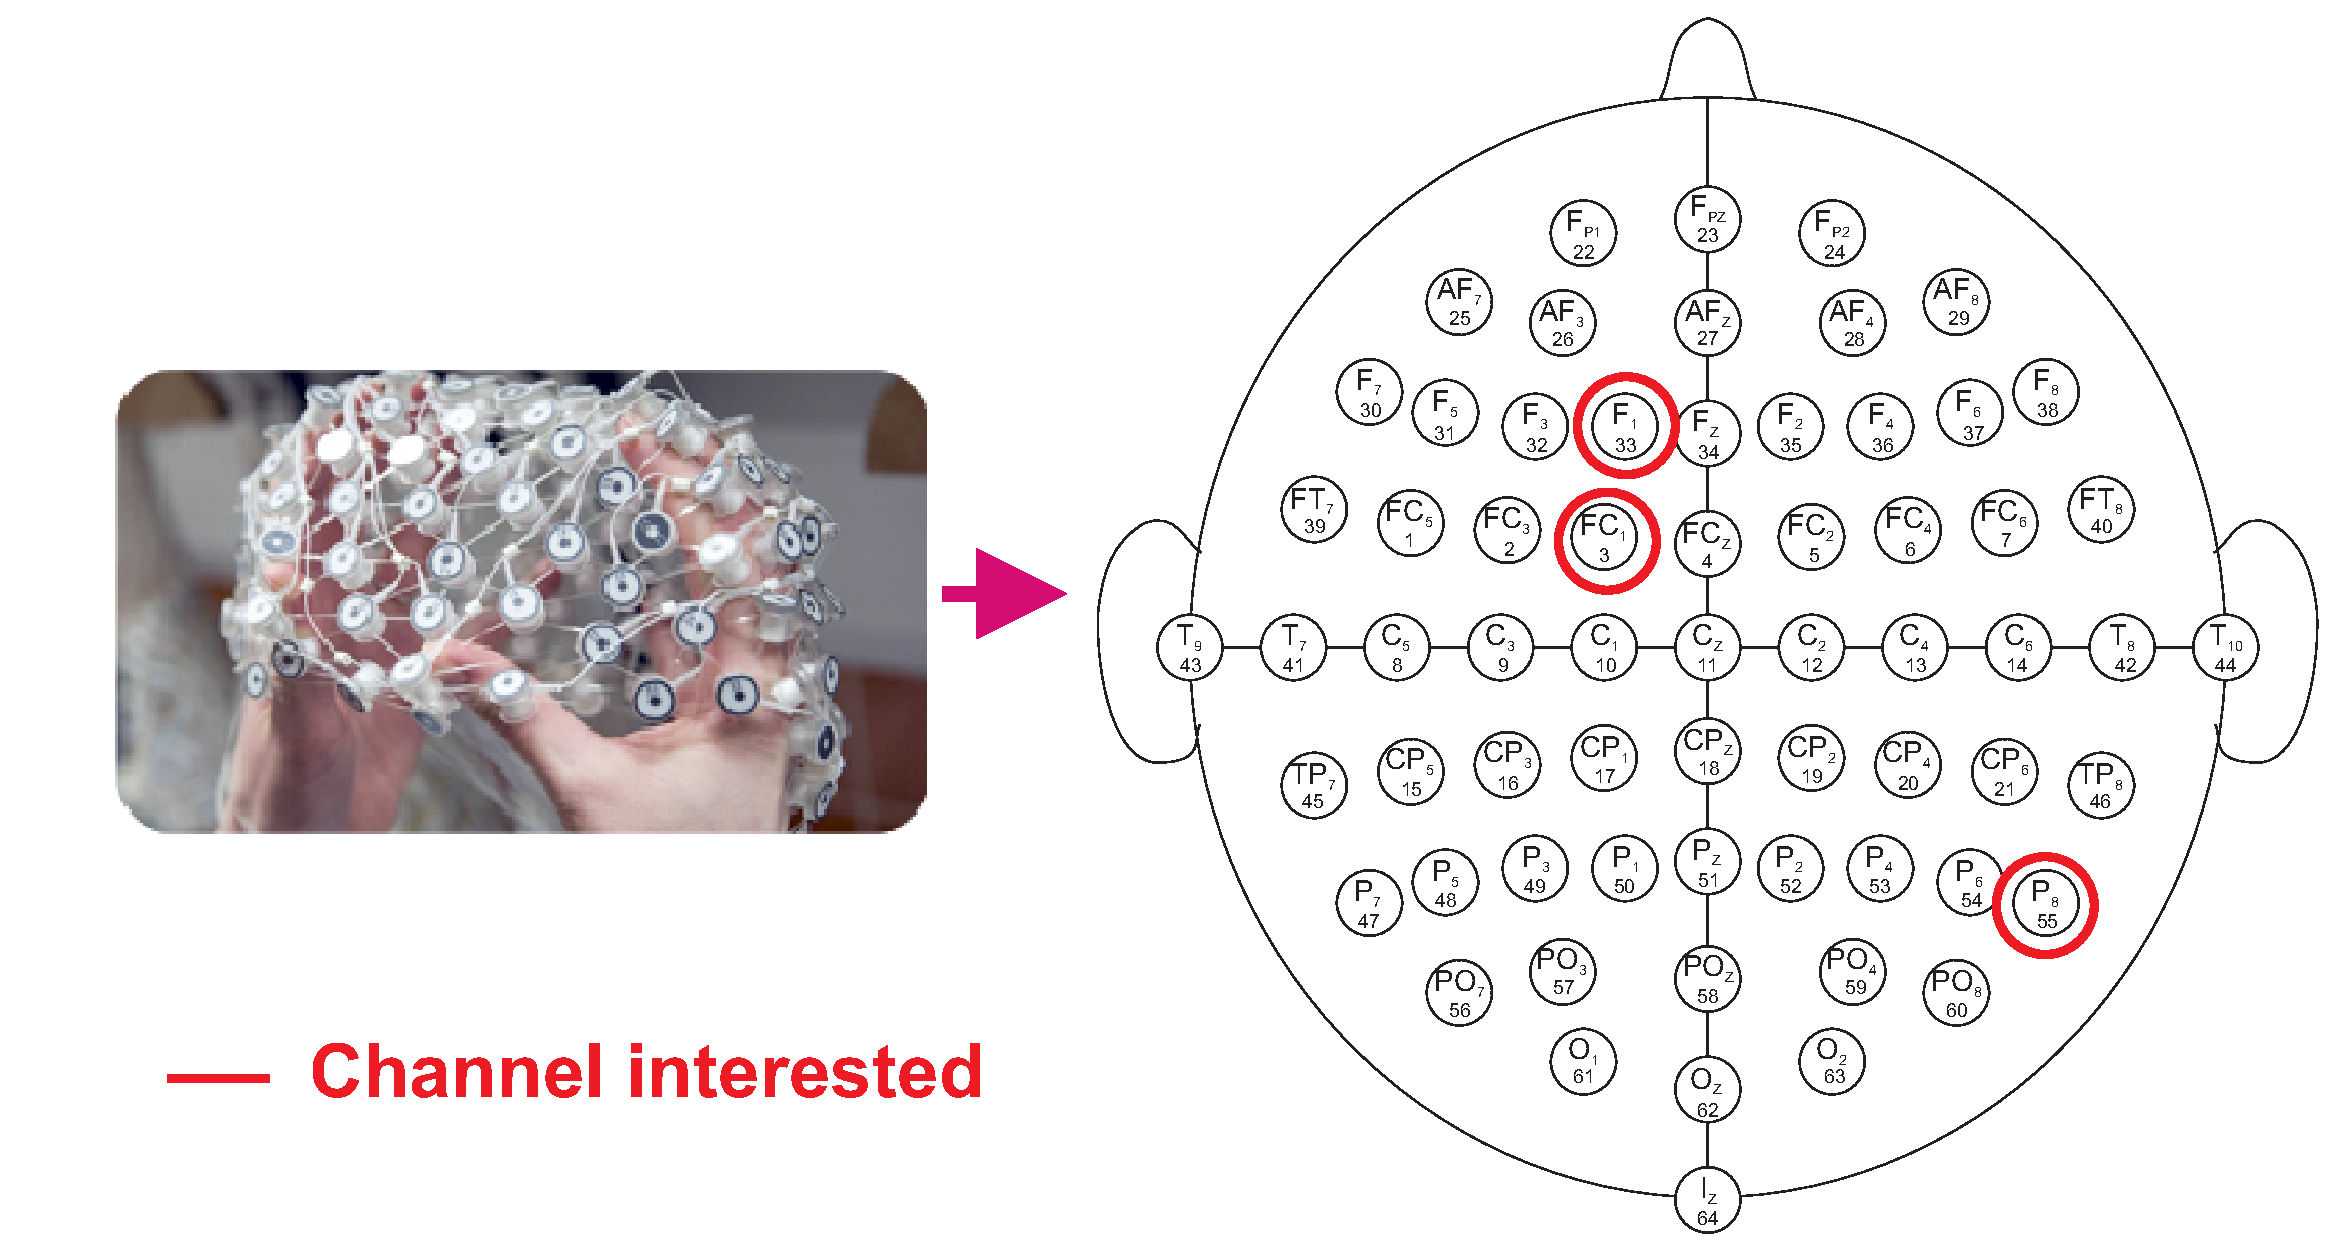
\includegraphics[width=0.9\columnwidth]{eeg.eps}
\vskip -3mm
\caption{\textbf{The 64-channel geodesic sensor distribution for measurement of EEG.}}\label{fig:eeg}
\vskip -5mm
\end{figure} 
 
To make the discussion more concrete and exemplify the mathematical formalism, we  investigated the statistical properties of a set of primary physiological processes (i.e, muscular, cardiac and neural processes). More specifically, we analyze the intramuscular EMG (iEMG), EEG and ECG signals from realistic clinical experiments. 
 
The iEMG signals are collected at different sites of the forearm muscles as shown in Figure~\ref{fig:emg}: (i) extensor digitorum (ED); (ii) flexor digitorum profundus (FDP); (iii) abductor pollicis longus (APL); (iv) flexor pollicis longus (FPL); (v) pronator teres (PT) and (vi) supinator (SUP), when the subject is asked to relax 6 seconds, then do the finger flexion at a consistent strength for 10 seconds. The ADInstruments data acquisition system sampled the iEMG at 4 KHz.

The EEG signals are recorded by a 64-channel electroencephalogram acquisition system shown in Figure~\ref{fig:eeg} that monitors the brain activity of 109 subjects when they are performing motor and imagery tasks upon noticing objects appearing on the screen~\cite{Physio_EEG}. Each subject is asked to open and close the corresponding fists or feet as a function of where the target appears. Each individual performed 14 experimental runs consisting of one minute with eyes open, one minute with eyes closed, and three two-minute runs of interacting with the target. The data set is collected by BCI2000 system with a sampling rate of 160Hz.
\begin{figure}%[htb]
\centering
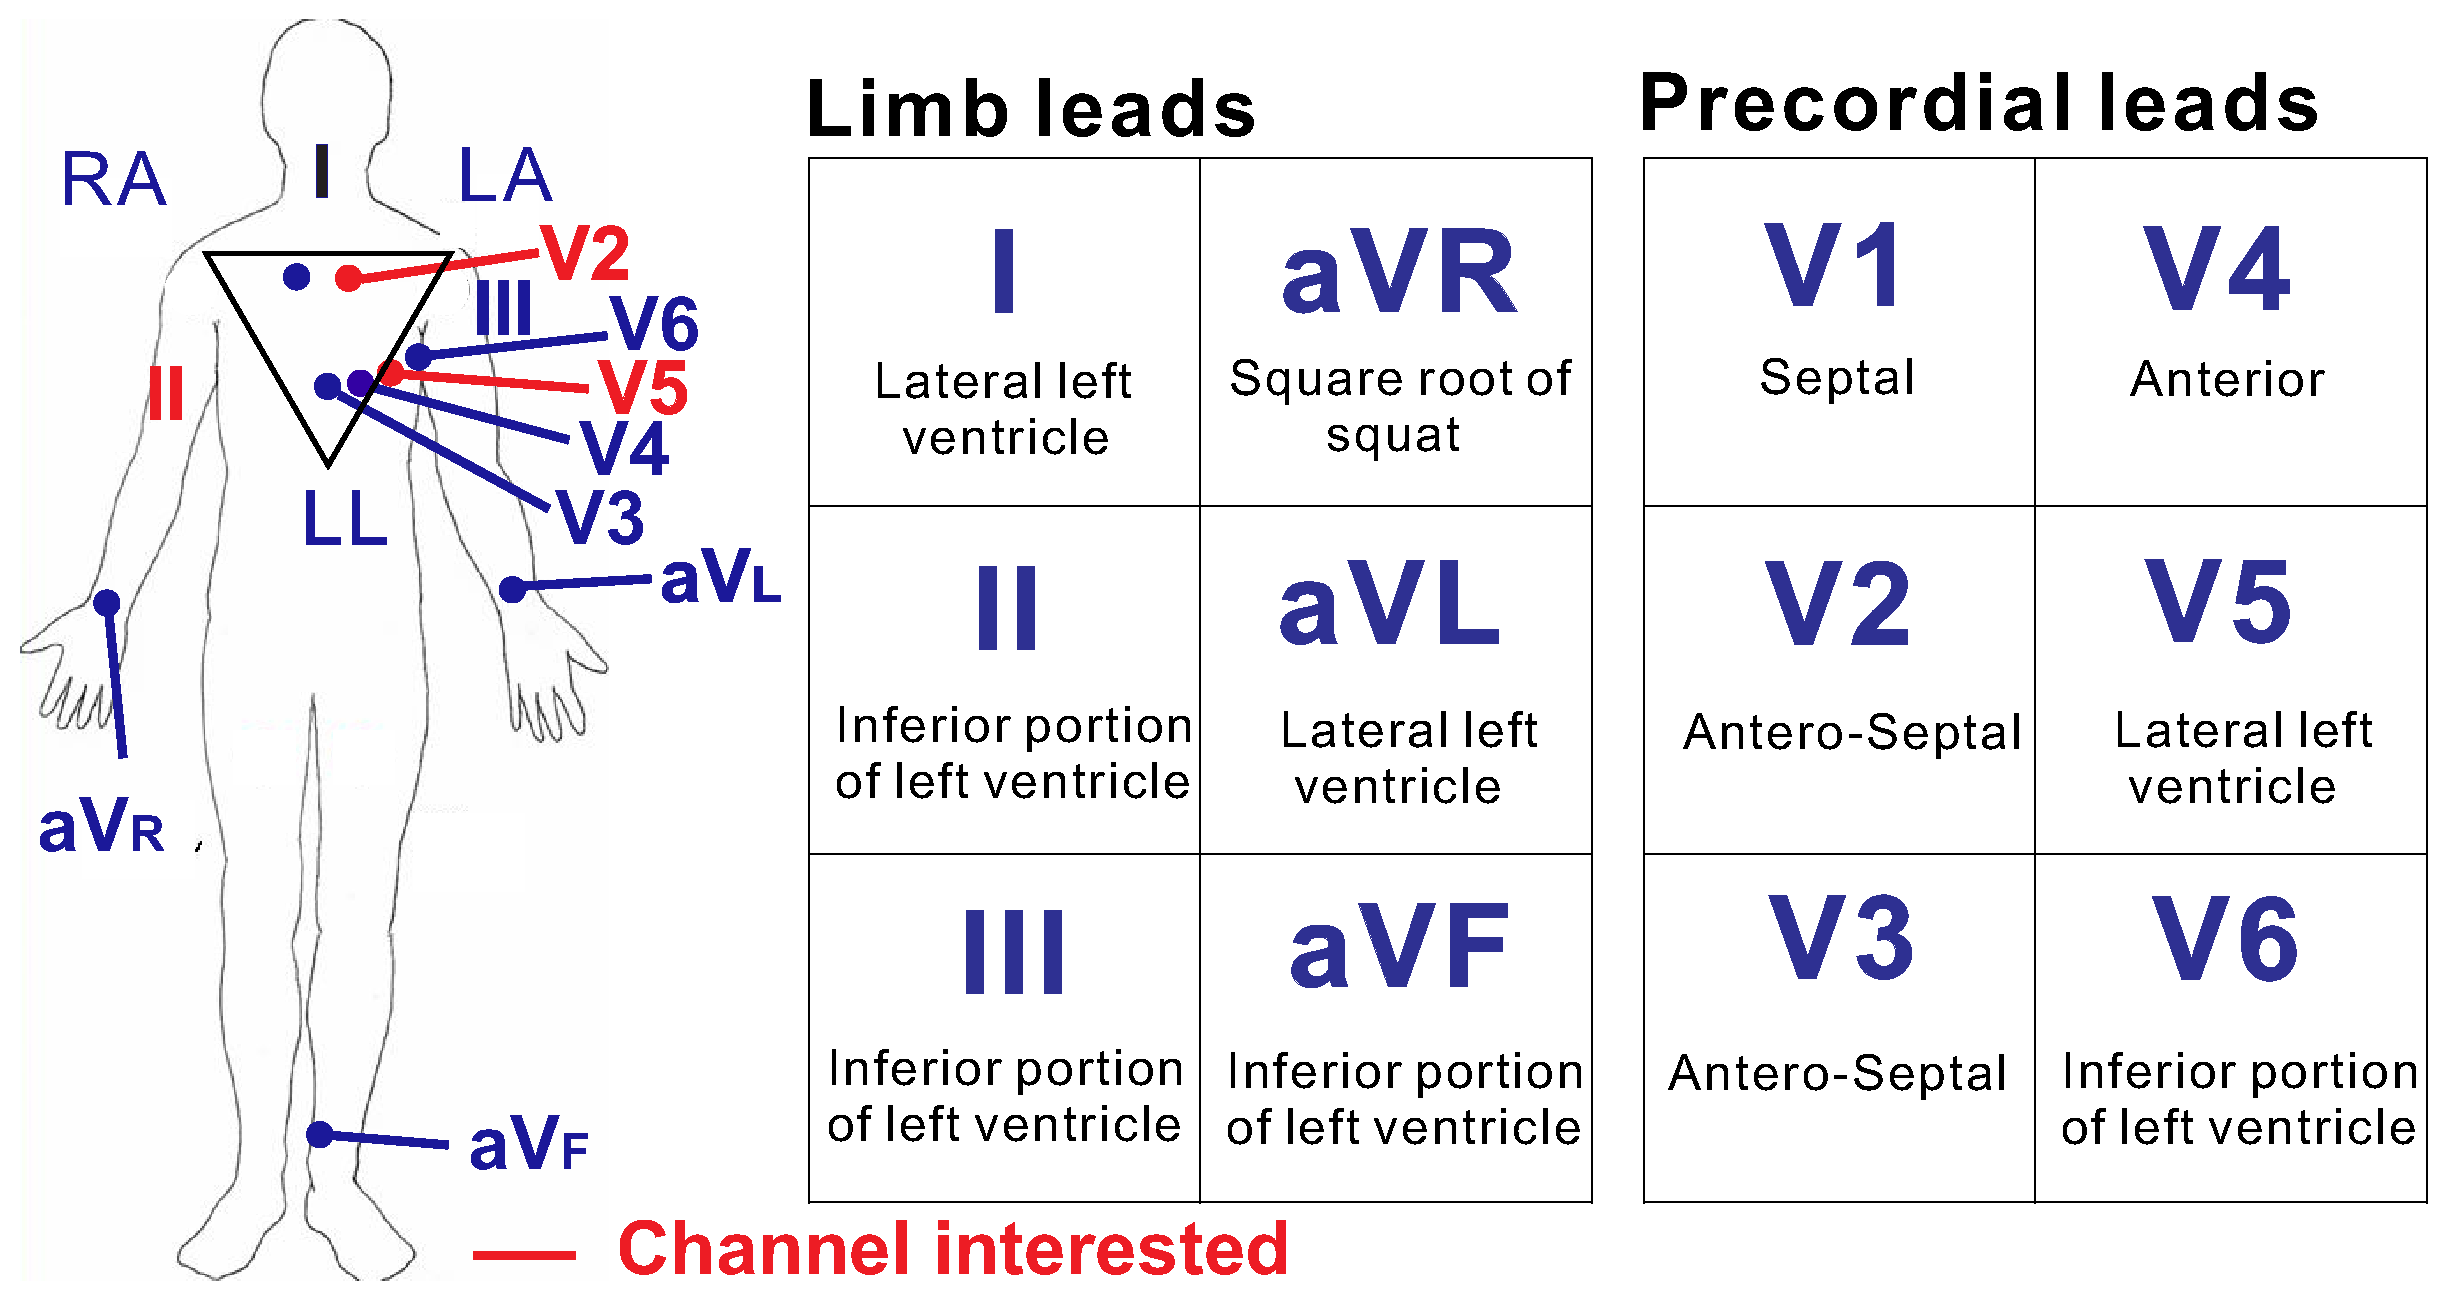
\includegraphics[width=0.9\columnwidth]{ecg.eps}
\caption{\textbf{The deployment of 12-lead ECG system used in the experiment is shown. }}\label{fig:ecg}
\vskip -6mm
\end{figure} 
The raw clinical ECG data was extracted from the PTB diagnostic ECG database~\cite{bousseljot1995nutzung}. Data on $52$ healthy subjects (13 women, age $48\pm 19$ and $39$ men, age $42\pm 14$) was obtained by the National Metrology Institute of Germany. Each subject’s record includes 15 different signals simultaneously acquired: the conventional 12-lead (I, II, III, aVR, aVL, aVF, V1, V2, V3, V4, V5, and V6) and 3 Frank orthogonal leads (VX, VY, and VZ) as shown in Figure~\ref{fig:ecg}. Each signal is digitalized at 1000Hz, with a signal bandwidth of 0Hz to 1KHz and with 1 uV LSB resolution. 
\subsection{Investigation of Non-Exponential System Dynamics}
\begin{figure}[!htb]
\centering
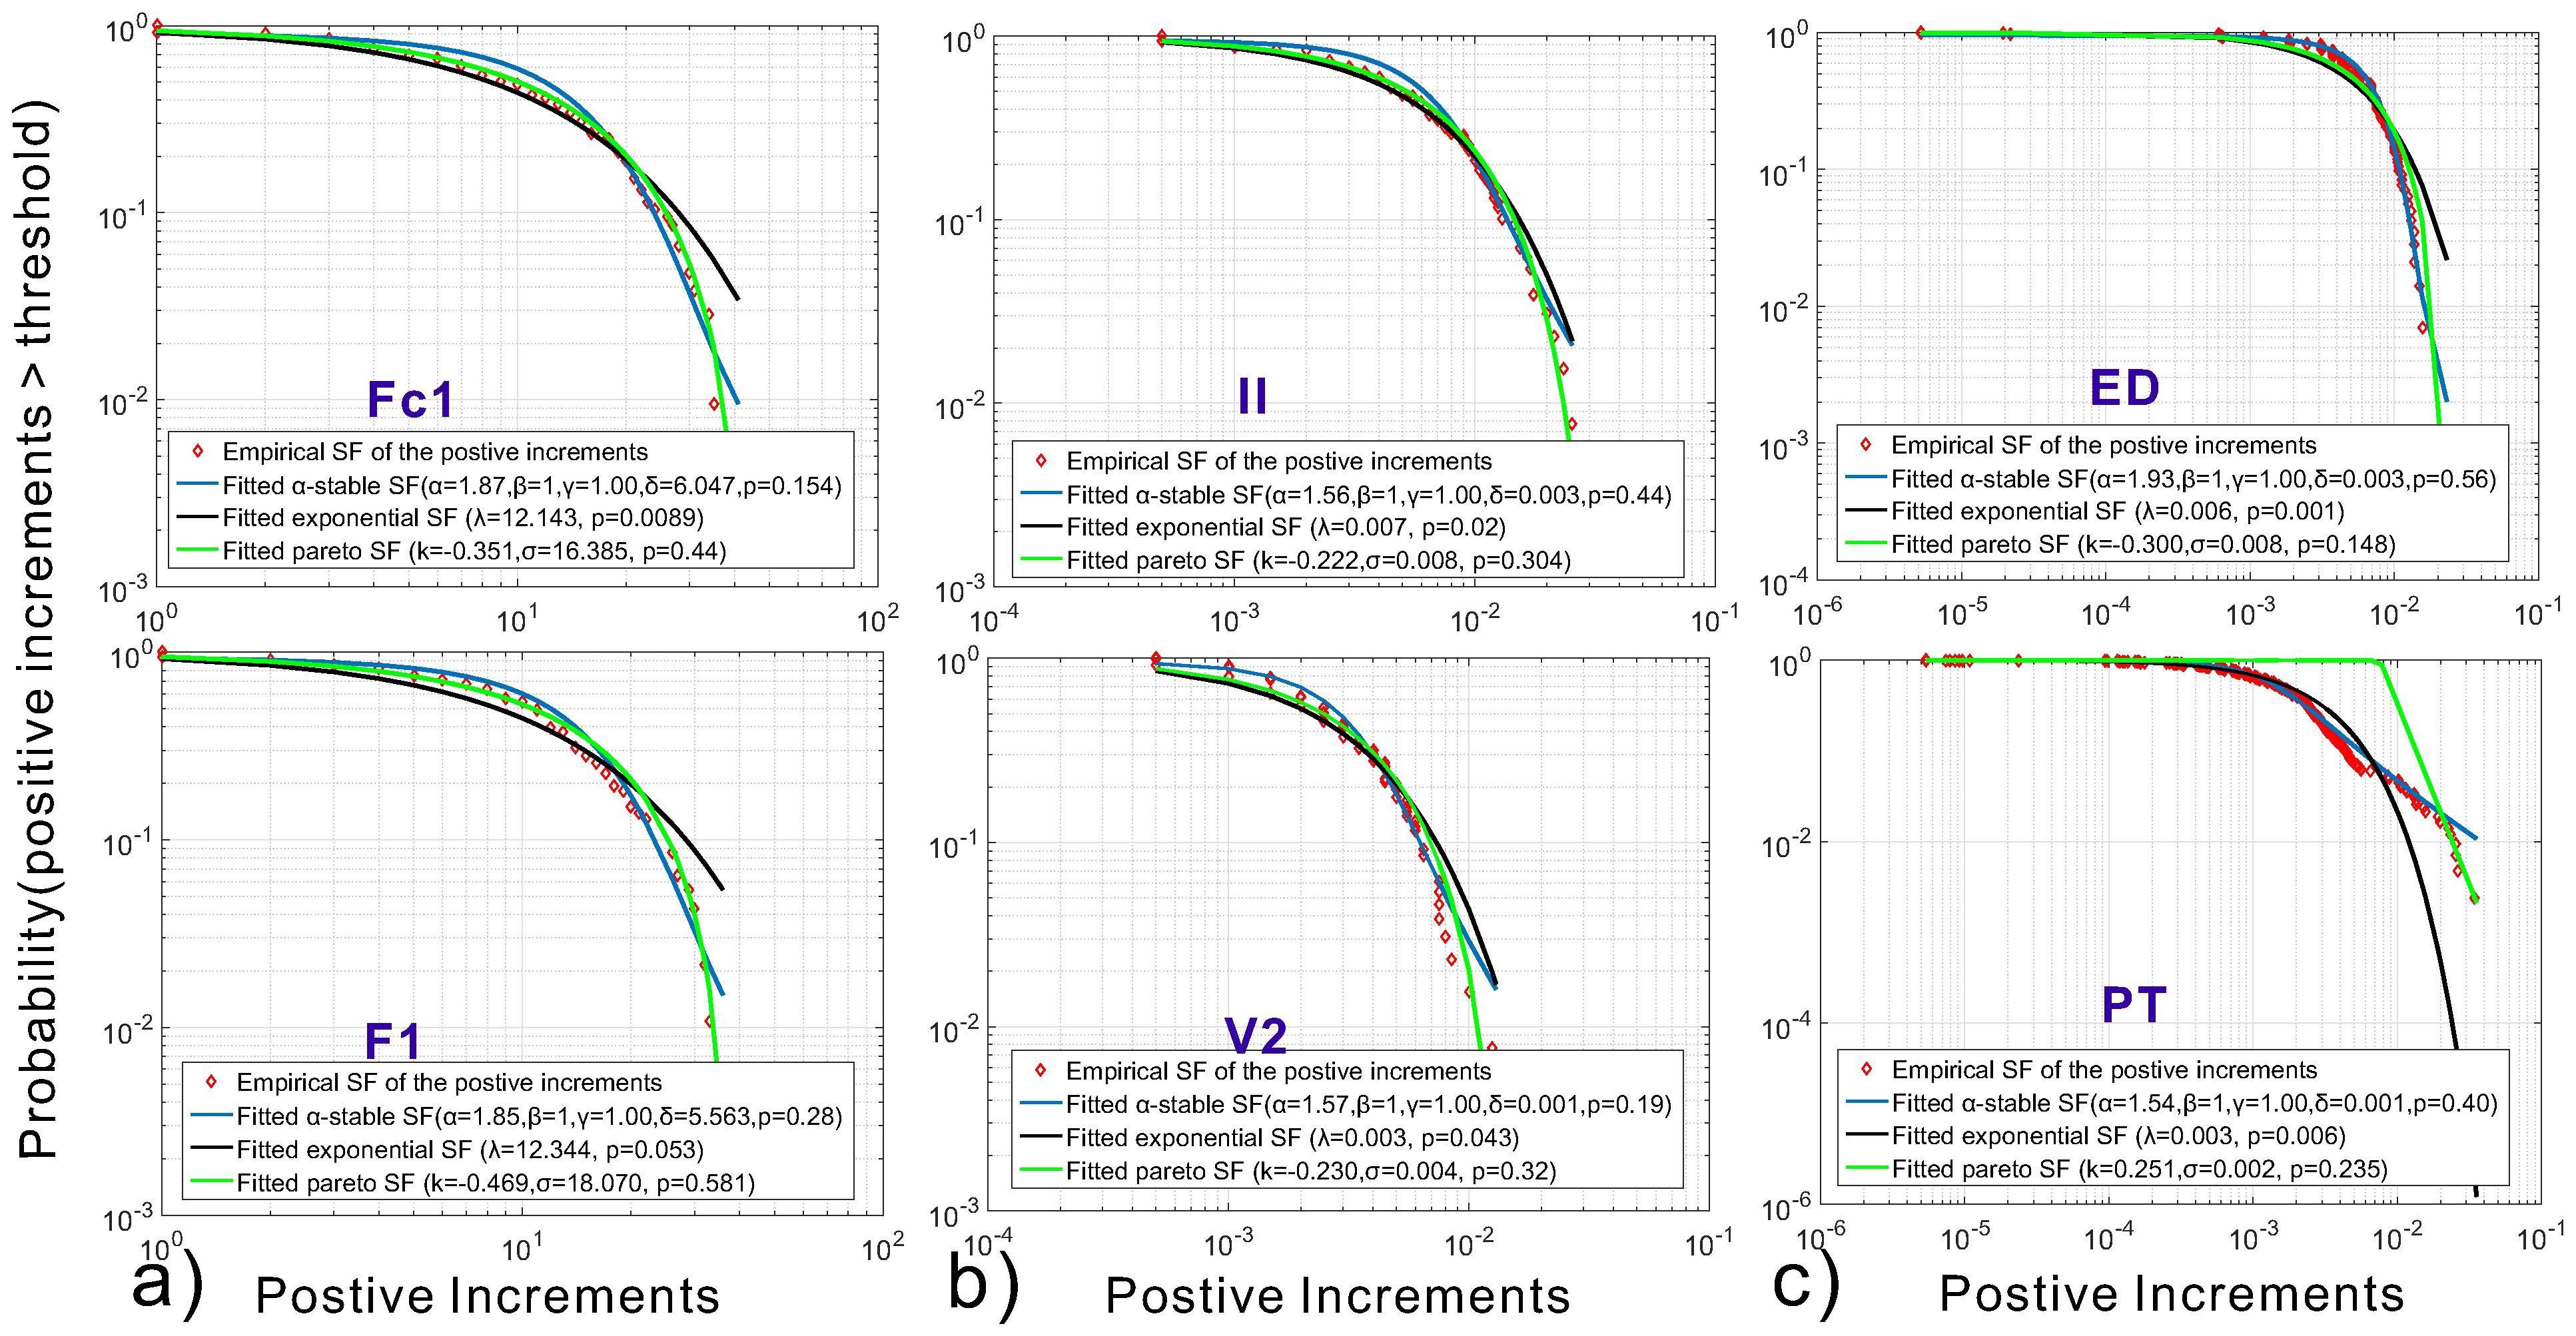
\includegraphics[width=1\columnwidth]{stats_overall_2.eps}
\vskip -3mm
\caption{\textbf{Empirical survival cumulative distribution functions and maximum likelihood best fitting $\alpha$-stable, exponential and Pareto distributions for magnitude increments in selected EEG, ECG and EMG channels. Figure (a)-(c) show the probabilities of the positive increments in magnitude exceeding a threshold value. P-value is obtained by performing a two-sample Kolmogorov-Smirnov test with the null hypothesis that the measurements come from the same distribution as the postulated $\alpha$-stable, exponential or Pareto distribution.}}\label{fig:stat_result}
\vskip -5mm
\end{figure}  

In the first set of experiments, we study the stochastic nature of magnitude increments (positive and negative) in all physiological processes considered to distinguish between exponential and power law behavior or between Gaussian and non-Gaussian cases. More specifically, we perform a statistical analysis to first estimate the empirical cumulative distribution function (CDF) and its support of the physiological process magnitude positive and the absolute value of negative increments. By fitting the measurements to the postulated stochastic models, we estimate the parameters of \textbf{i)} an $\alpha$-stable distribution, \textbf{ii)} exponential distribution and iii) Pareto distribution via maximum likelihood method. Then the CDFs of three stochastic models are generated based on the estimates of the model parameters.  

To quantify the statistical confidence of model fitting, we performed the two-sample Kolmogorov-Smirnov test between the measurements and the generated stochastic processes with identified $\alpha$-stable, exponential and Pareto distribution parameters. The null hypothesis assumes the measurements come from the same distribution as the postulated distributions with significance of 0.05. As a case study, we report the results of a selected set of physiological channels from the subjects that best illustrate their stochastic natures. Both positive and negative increments are studied and we visualize the experiments considering the positive increments in Figure~\ref{fig:stat_result}. Figure \ref{fig:stat_result}.(a-c) show how two models fit to the empirical survival function (SF) of a set of EEG (a), ECG (b) and iEMG (c) signal channels in the corresponding experiments, respectively. The interested channels are highlighted in Figure~\ref{fig:emg}-\ref{fig:ecg}. In all subfigures, the red squares correspond to the empirical SF, the blue lines, the black lines and the green lines represent the best-fitted $\alpha-$stable distribution, exponential distribution and Pareto distribution, respectively. The retrieved model parameters and p-values are reported in both the plot legends and Table \ref{tab:pos_neg}. 

By examining the figures, we can make several important observations: i) The null hypothesis that the positive increments follow an exponential distribution is rejected in all physiological channels we considered with p-value ranging from $0.001$ to $0.043$. This suggests that magnitude variation over time domain strongly contradicts with an exponential law which is a well-adopted assumption in previous work. 

ii) The p-value well coincides with our visual inspection that the exponential SF fitting (black lines) deviates the empirical SF in all the channels considered. Instead, the Pareto distribution and the $\alpha$-stable fitting better represent the stochastic properties of the signal variations over time in all channels. This suggests the existence of fractality which is governed by a power-law distribution as postulated by equation~(\ref{multidimensionalTP}), which also coincides with our following observation.

 iii) For all channels that can be better characterized by an $\alpha$-stable distribution or Pareto distribution, the estimated stability parameters $\alpha$ are all smaller than 2 where $\alpha=2$ corresponds to a Gaussian process. For $\alpha < 2$, stable distributions have one tail (when $\alpha < 1$ and $\beta = \pm 1$) or both tails (all other cases) that are asymptotically \textit{power laws} with heavy tails. This is best illustrated in FDP and PT channel of iEMG signals where the empirical distribution fits well to the $\alpha-$stable distribution up to a certain transition point where the empirical SF starts to obey the Pareto distribution (i.e., power-law). This suggests the existence of fractality in these physiological processes which is aligned with our analytical prediction made by Theorem 1, hence justifying the application of the proposed fractal dynamical state equation described in equation~(\ref{vectorARFIMA1}). The similar conclusion can also be reached by investigating the stochastic properties of the negative increments (see Table~\ref{tab:pos_neg}) in physiological processes.
\subsection{Efficacy Evaluation of FDSE for Physiological Processes}
\begin{figure}%[!htb]
\centering
\includegraphics[width=1\columnwidth]{overall_2.eps}
\vskip -5mm
\caption{\textbf{Fitting the model to physiological measurements of EEG, ECG and iEMG considering i) FDSE with no coupling matrix $A$, ii) FDSE with coupling matrix $A$ and iii) Vector ARMA model with no fractal exponents.}}\label{fig:exp_result}
\vskip -4mm
\end{figure}  

\begin{table}[ht]
\caption{KS-test and ML best-fitting parameters of $\alpha$-stable, exponential and Pareto distributions for selected channels}
\vskip -4mm
\begin{center}
\scalebox{0.72}{
\begin{tabular}{|c|c|c|c|c|c|c|c|c|c|c|c|c|c|c|c|}
    \hline
    \multirow{2}{*}{Channel}&\multicolumn{6}{c|}{Positive increments} & \multicolumn{6}{c|}{Negative increments} \\
    \cline{2-13}
    &$\alpha$,$\beta$,$\gamma$,$\delta$&$p_{stbl}$&$\lambda$&$p_{exp}$&k,$\sigma$&$p_{par}$&$\alpha$,$\beta$,$\gamma$,$\delta$&$p_{stbl}$&$\lambda$&$p_{exp}$&k,$\sigma$&$p_{par}$\\
    \hline
    Fc1&1.87,1,1,6.05&0.15& 12.14& 0.0089& -0.35,16.39& 0.44 &1.56,1,1,5.56& 0.08& 14.47& 0.071& 0.39, 20.04& 0.18\\
    \hline
    F1& 1.85,1,1,5.56 &0.28& 12.34& 0.053& -0.47,18.07& 0.58& 1.89,1,1,6.02 & 0.15& 11.29& 0.05& -0.43,16.18& 0.73\\
    \hline
    P8& 1.57,1,1,4.62& 0.19& 11.38& 0.0025& -0.19, 13.56& 0.16& 1.88,1,1,6.17& 0.01& 11.2& 0.03& -0.25,14.03& 0.16\\
    \hline
    II& 1.56,1,1,0.003& 0.44& 0.007& 0.02& -0.22, 0.008& 0.30& 1.69,1,1,0.003& 0.24& 0.006& 0.0089& -0.20, 0.007& 0.21\\
    \hline
    V2& 1.57,1,1,0.001& 0.19& 0.003& 0.043& -0.23,0.004& 0.32& 1.8,1,1,0.002& 0.05& 0.004& 0.01& -0.40,0.005& 0.38\\
    \hline
    V5& 1.4,1,1,0.001& 0.15& 0.003& 0.0017& -0.19,0.004& 0.33& 1.93,1,1,0.002& 0.01& 0.003& 0.047& -0.42,0.005& 0.49\\
    \hline
    ED& 1.93,1,1,0.003& 0.56& 0.006& 0.001& -0.30,0.008& 0.15& 1.92,1,1,0.003& 0.1& 0.005& 0.034& -0.29,0.007& 0.65 \\
    \hline
    FDP& 1.09,1,0.59,0.004& 0.36& 0.014& 0.01& 0.18,0.011& 0.22 &0.49,1,1,0.003& 0.15& 0.021& 0.0001& 0.87,0.007& 0.47\\
    \hline
    PT& 1.54,1,1,0.001& 0.4& 0.003& 0.006& 0.25,0.002& 0.24& 1.41,1,1,0.001& 0.37& 0.002& 0.004& 0.051,0.002& 0.68\\
    \hline
\end{tabular}}
\end{center}
\label{tab:pos_neg}
\vskip -5mm
\end{table}
The investigation of the stochastic characteristics of the processes considered verified the existence of non-Gaussian and fractality (non-linearity) in the physiological systems. Therefore, the dynamical behaviors of these systems in time and spatial domain can not be accurately described by the conventional methods that assumes a stationary and Markovian system state equation with short-term memory. In what follows, we present the second set of experiments where we are interested in the spatial (i.e, interdependency across multiple channels) and temporal (i.e., how previous system state passes down its influence to current system dynamics) dependency structure of the physiological processes. We evaluated the capability of the proposed FDSE in capturing the complex dynamical behaviors of physiological processes. More precisely, we employed a least-square error estimator proposed in~\cite{xue2016spatio,xue2016minimum} to identify the model described by equation (\ref{vectorARFIMA1}). After the identification of the model, we evaluate the model adequacy by comparing the physiological measurements and predicted model output as goodness-of-fit metrics. 

To compare with the Vector ARMA (VARMA) model and understand the significance of coupling the fractal exponents into FDSE (i.e., considering the long term memory in system state dynamics), we report three experimental settings: i) only fractal exponents $\beta$ are considered (i.e., assuming an identify matrix for $A$ in equation (\ref{vectorARFIMA1})); ii) only coupling matrix $A$ is considered (i.e., assuming $\beta_{i}=1$ which reduces to VARMA type model) and iii) both coupling matrix and fractal exponents $\beta$ are considered (i.e., FDSE). We show the comparison results of a selected set of channels from EEG (a), ECG (b) and iEMG (c) measurements in Figure~\ref{fig:exp_result}, respectively. The blue lines show the actual measurements. The orange lines represent the predicted model output where only fractal exponents are considered (i.e, setting i). The yellow lines and the magenta lines correspond to setting ii and iii, respectively. We use the system identification approach proposed in \cite{xue2016spatio}. The estimated fractal exponents range from $ 0.30$ to $0.66$, $0.94$ to $1.19$ and $0.18$ to $0.61$ for EEG, ECG and iEMG signals, respectively, hence verifying the existence of fractality.

 Two key observations can be made for Figure~\ref{fig:exp_result}: i) In all experiments we considered, the efficacy of incorporating the fractal exponents that captures the long-term memory effect in system dynamics can be best illustrated by the comparison between the predicted model output and actual measurements. In spite of the difference in magnitude, the predicted model output stays close to the actual measurement in terms of preserving critical system state transition behaviors. Intuitively, the predicted model output preserves turning points and the envelope of the state dynamics of actual physiological processes. This is primarily important for construction of a time-series model capable of characterizing the physiological processes. Vital changes in bio-markers of the physiological system usually correspond to \textit{infrequent anomalies} (e.g., the abrupt decrease/increase in blood glucose/blood pressure or excessive brain activity caused by epilepsy). The failure of the model in capturing such vital changes translates to false negative errors and might lead to irreversible undesired consequences. In contrast, the fitted VARMA models without considering the long-term memory have the tendency to smooth away the sudden changes in model output in order to minimize least-square errors as a consequence of the regression process.
 
 ii) Comparing the goodness-of-fit between FDSE models with and without considering coupling matrix $A$ that encodes the interdependency across different channels leads to interesting findings. As shown in the figure, the FDSE without matrix considering $A$ tends to overestimates the signal magnitude as a result of accumulating the influence of the previous system states over a long time course. In contrast, FDSE model with coupling matrix $A$ in all experiments aligns well with the actual measurements suggesting its adequacy in characterizing the physiological processes. The performance difference can be understood as follows: the FDSE assuming an identity matrix $A$ has no knowledge of how coupled physiological processes contribute to the state transition dynamics of each other. As a result, given a specific channel, the estimation process tries to compensate the contribution from other channels by assuming a long lasting influence from the previous system states. By incorporating the matrix $A$, the predicted model output is well regulated to adequately fit to actual measurements by coupling the interdependency between different channels of the physiological signals.
\section{Summary}
\label{Conclusion}
Understanding the implications of the degree of nonlinearity and the nature of fractality (i.e., distinguishing between fractality in the magnitude increments (space) of one variable with respect to other variables and the fractality in the inter-event times) represents the motivation of this work. We generalize the linear / nonlinear dynamic causal approaches, by adopting a statistical physics inspired probabilistic description of various processes representing the evolution of a complex system and incorporating the statistics of the magnitude increments and the inter-event times into the mathematical expression of the master equation. 

First, this new approach allows to capture the power law and nonlinear interactions that exist between the magnitude increments and the inter-event times of one stochastic process on one hand, and the inter-dependencies between the magnitude increments and the inter-event times of one process and other processes, on the other hand. Second, it provides a mathematical strategy for modeling of complex systems whose dynamics exhibits a mixture of Markovian and non-Markovian evolution. Relying on conditional probabilistic description on how ordered sequence of magnitude increments and the inter-event times affect the overall system dynamics allows to define new multivariate causal inference techniques that take into account the non-Markovian nature of the dynamics. This is left for future work. Moreover, it allows to mathematically justify the adoption of a class of mathematical model that could potentially complement current Bayesian model selection strategies. The presented mathematical framework could be enriched by combining it with other techniques from statistical machine learning and signal processing for developing new modeling strategies for complex interdependent networks. Third, the proposed causal modeling of complex dynamics can be integrated as the core of the cognizant cyber-physical systems in a widely ranged CPS applications to be able to understand, describe, predict and control the underlying physical processes.


\chapter{Spatio-Temporal Fractal Model for a CPS Approach to Physiological Systems}
\label{cha:ch3}
Advances in the physical sciences and engineering enable the development of cyber-physical systems (CPS) to understand, interface / interact and engineer physical (biological) world (systems). The CPS paradigm refers to a broad class of smart systems with deeply embedded cyber capabilities for sensing, monitoring, and communicating the accumulated large amounts of data about the physical world to computational nodes for real-time analysis, interpretation and determination of closed-loop control strategies \cite{Abdelzaher}\cite{Baheti}\cite{Bogdan}. Although the synergetic coupling of physical and cyber processes has a tremendous impact on a broad application domain (e.g., environmental, healthcare, avionics, smart transportation / buildings / cities), it also raises a few grand challenges: What is the appropriate \textit{modeling framework} that captures the CPS characteristics and facilitates the analysis, design and optimization of CPS? What \textit{compact yet accurate modeling} techniques that account for spatio-temporal complexity and fractal properties should be developed to enable the design of large-scale autonomous (or semi-autonomous) CPS? What are the data mining strategies that meet the real-time CPS requirements? How can the cognitive control of human brain be understood and be enabled within the CPS architectures?

To address these challenges, we turn our attention to biological systems and get inspiration from understanding the dynamics and functionality of human brain to enable a more efficient and safer human-to-cyber-to-physical interaction. From a healthcare perspective, understanding and mining brain activity can be beneficial for developing CPS-based therapies (e.g., brain-machine-body interfaces (BMBI)) for brain disorders. As stated in \cite{He}, we use a rich neurotechnology to measure the brain activity, but lack mathematical models, algorithms and computational tools for understanding neural-muscle data, deciphering disease indicators, explaining brain disorders, identifying clinical therapies and enabling complex human-to-cyber interactions. From control perspective, understanding and modeling the human brain cognition could help us define the principles of autonomous systems design. For manufacturing and smart things, thought-controlled robots that can interact with our collective cognitive efforts could contribute to not only higher yield/performance, but also safer environments. Thought-control systems could prove essential for cleanup operations in dangerous environments (e.g., nuclear reactors) or for maintaining high ecological standards.\\
\begin{figure}%[htb!]
\centering
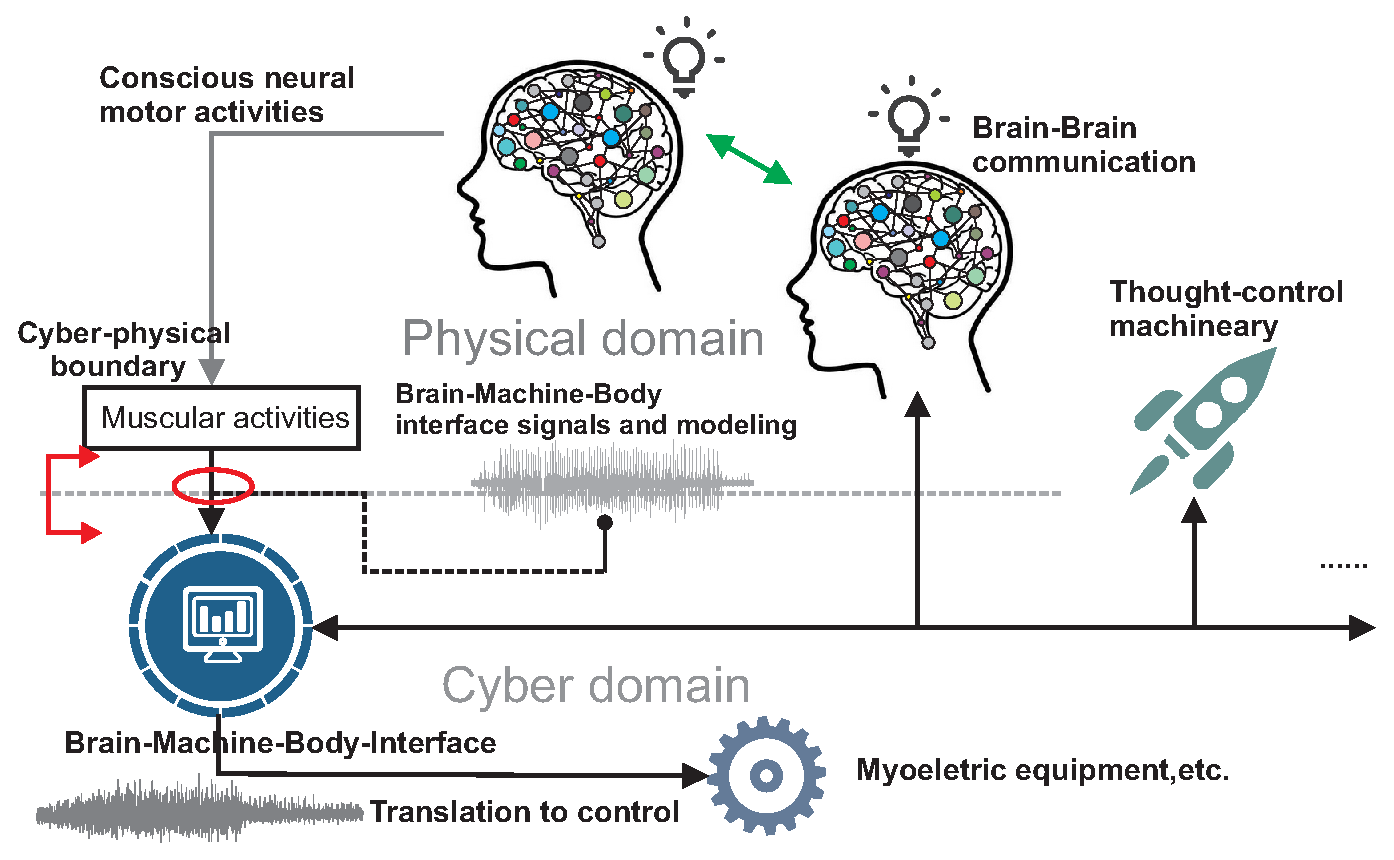
\includegraphics[width=0.94\columnwidth]{brain-brain-interface.eps}
\vspace{-3mm}
\caption{\textbf{Cyber-physcial system for Brain-Machine-Body interfaces}}\label{fig:BMBI}
\vspace{-7mm}
\end{figure}
\indent Traditional approaches for developing decoding algorithms of brain dynamics (converting spiking neural activity from motor cortex into muscle activity and kinematics of a prosthetic arm) have mainly focussed on determining a mapping function from some observations of neural and muscle activity (training data) by minimizing a specific error metric on testing data. Despite some successes, these approaches have neglected some important features of brain-muscle dynamics: (\textit{i}) A cognitive operation may activate a brain region, but the converse operation of activating that same region does not imply that the cognitive process is actually occurring. This implies that assuming instantaneous activation may offer a simplistic view and that the spatial correlation structure and functional dependency between multiple brain regions must be taken into account. (\textit{ii}) Brain activity is not random. Even though many studies assumed a high degree of randomness in the neural dynamics for the purpose of employing statistical averaging, the actual brain dynamics and its coupled physiological processes proved to posses fractal characteristics. Simply speaking, the neural and muscle activity cannot be modeled as short-range dependent processes, but rather their long-range dependence should be accounted for improving modeling accuracy and prediction capabilities. 
\begin{figure} %[htb!]
\centering
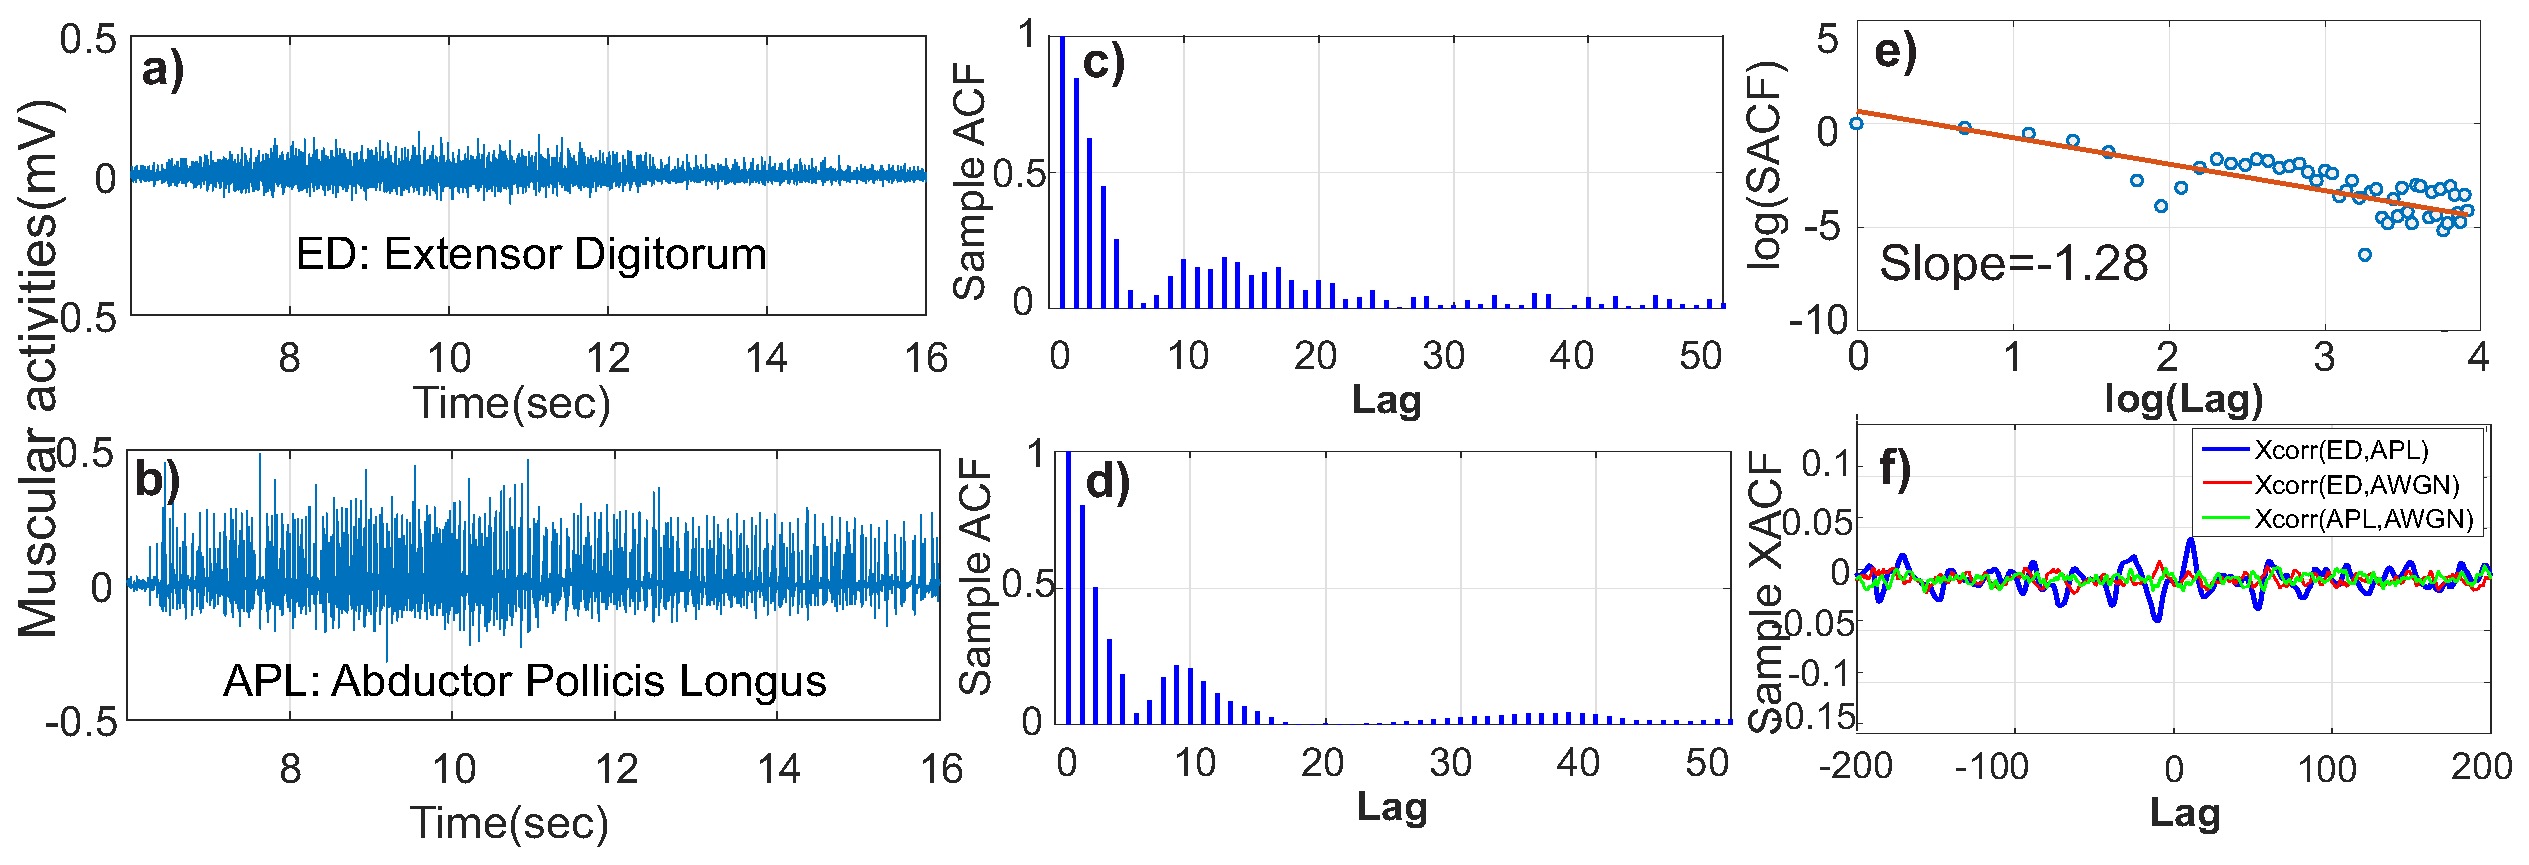
\includegraphics[width=1\columnwidth]{raw_data_thumb_abct_revision.eps}
\vskip -3mm
\caption{\textbf{a-b) The iEMGs from two muscles (ED and APL) are measured when the subject is abducting the thumb for 10 seconds after 6-second relaxing. c-d) The SACF decays hyperbolically rather than exponentially proving a long-range memory. e) The SACF $log-log$ plot of ED iEMG measurements against lags shows a \textit{power-law} behavior. f) The SXACF between the iEMG signals proves the spatial interdependence over time.}}\label{fig:overview}
\end{figure} 
\section{Related Work and Novel Contribution}
Probing brain's activity for the purpose of decoding its cognitive process, explaining its interaction with overall body (e.g., muscles) and controlling the movement of arms originated in the 1960's with the pioneering work of Evarts \cite{Evarts}.  More recently, Donoghue and co-workers designed the BrainGate which allowed a tetraplegic patient with spinal cord injury perform simple movements \cite{Hochberg}.    

Going beyond performing simple tasks requires advanced mathematical and algorithmic approaches for decoding brain-muscle activity. Current approaches for the analysis of electroencephalographic (EEG), electrocortigraphic (ECoG) and electromyographic (EMG) signals can be classified into two classes: linear (e.g., linear estimator \cite{Collinger}\cite{Salinas}, population vector \cite{Velliste}, Wiener filter \cite{Ethier}, Kalman filter \cite{Kim}, recalibrated feedback intention-trained Kalman filter \cite{Fan}) and nonlinear (e.g., artificial neural networks \cite{Sanchez}\cite{Sussillo}, particle filters \cite{Shoham}). 

To enhance the BMBI capabilities and performance, we must address the following challenges: (\textit{i}) Real-time parameter identification of the decoder algorithm. We propose a closed-loop spatio-temporal fractal (STF) model that interacts with BMBI user. This overcomes the suboptimal performance of algorithms that are based on offline cross-correlation validation. (\textit{ii}) Use the neuromuscular spatial dependencies and their fractal dynamics to develop a model of the BMBI at runtime for the purpose of analysis, prediction and control. Many of the current approaches ignore these unique aspects.
%(\textit{i}) Identifying the parameters of the decoder algorithm via offline cross-validation can not only be time consuming, but also lead to poor performance or suboptimal real-time control. Consequently, we advocate for adopting a closed-loop \textit{spatio-temporal fractal} (STF) modeling  approach that continuously interacts with the BMBI user. (\textit{ii}) Many of the current approaches ignore the fractal characteristics and unique aspects of BMBI. In contrast, our STF modeling framework aims to identify the characteristics of the BMBI (spatial dependencies between neural and muscle activity and their fractal dynamics) and develop a model of the BMBI at run-time for the purpose of analysis, prediction and control. %(\textit{iii}) A major problem in CPS based BMBI systems is the state-space explosion (i.e., the number of states required to describe the state of the system tend to increase exponentially). To avoid such situation, we develop an optimization and signal processing algorithmic approach that seeks to determine over predefined windows of time the minimum number of state variables that are required to accurately model and predict the CPS dynamics. 

To illustrate the discrepancies between the mathematical features of biological processes and the current employed memoryless models, we analyze the intramuscular EMG (iEMG) signals from clinical experiments(iEMG Recording study in courtesy of The Alfred Mann Foundation)  where 3 tested healthy subjects are asked to perform forearm movements. The iEMG signals are recorded at different sites of the forearm muscles: (1) extensor digitorum (ED), (2) flexor digitorum profundus (FDP), (3) abductor pollicis longus (APL), (4) flexor pollicis longus (FPL), (5) pronator teres (Pro), and (6) supinator (Sup) (see Figure \ref{fig:exp_setting} and section IV for experimental setup details). Figure \ref{fig:overview} shows 2 measured time series for 2 muscles (ED and APL) when the subject is asked to abduct the thumb at a consistent strength for 10 seconds before relaxing (a-b), the sample autocorrelation function (SACF) of the 2 signals (c-d), the $log$-$log$ plot of SACF of the signal collected from ED (e), and the sample cross-correlation function (SXACF) between the muscle time series (f). The individual analysis of iEMG signals via the SACF method (see Figure \ref{fig:overview}.c-e) shows that the SACF $\gamma(k)$ decreases for higher lags $k$ as a power law rather than as an exponential that corresponds to short-range memory or non-fractal models (including autoregressive (AR) models). This is best shown in Figure \ref{fig:overview}.(e) where the points corresponding to the $log(\gamma(k))$ scatter around a straight line as a function of $log(k)$, following a $log(\gamma(k))=const+\alpha log(k)$ expression. This demonstrates the existence of a correlated neural-muscular regulatory over long temporal horizons. 

To probe the spatial cross-dependency among biological processes, we measure the sample cross-correlation functions (SXACF) (see Figure \ref{fig:overview}.(f)). In contrast to uncorrelated signals (e.g., additive white Gaussian noise with zero SXACF), the SXACF analysis among iEMG signals demonstrates consistent interactive influence and reveals spatial \textit{long-term} dependencies. The amplitudes of the SXACF coefficients are fluctuating over a long temporal horizon which is not expected assuming short memory processes. Such long term memory effect can also be found in other neural and muscular signals and are not discussed here due to limited space. In summary, the analysis in Figure \ref{fig:overview} shows that even the simple movements of the thumb calls for a synergetic model of neural, muscular and cyber components as \textit{interdependent} networks. Alternatively, capturing such long term cross-dependent behavior associated to BMBI calls for the development of \textit{multivariate fractal} mathematical model within CPS. In light of these mathematical observations, we make the following contributions:

\indent \textbf{First}, we propose a \textit{data-driven multivariate fractal} model to capture the long-range memory and spatial cross-dependencies that exist between biological (neural, muscular) and cyber processes. By exploiting the fractal properties of the biological processes, the model can be learned within a CPS infrastructure at run-time from fewer measurements.

\indent \textbf{Second}, we develop an efficient algorithm for identifying the parameters of the proposed mathematical model and provide theoretical bounds concerning the minimum amount of samples that lead to good identification performance.

\indent \textbf{Third}, we investigate the effectiveness and accuracy of the proposed mathematical model, we contrast and highlight the benefits of our model with prior memoryless approaches and validate our model under clinical measurements and known biological facts from medical literature. This mathematical framework enables the understanding of cognitive control and development of advanced control techniques for CPS.   
\section{Spatio-temporal Fractal(STF) Modeling}
%In this section, we start with presenting the biological and physiological foundation of our proposed model by identification of multidimensional correlations that affect the cerebral-muscular synergies of BMBI. To make very concrete discussion, we keep aligning our proposed model with the realistic clinical experiments in capturing the mathematical structures of intramuscular electromyography (iEMG) signal which serves as an important direct information carrier of brain-body signaling system. In the experiments, we evidence the existence of sptio-temporal interplays and fractal properties by analyzing the brain-body interface signals. To best fit to the observed dynamics, we propose a cross-related fractal autoregressive model for characterization of the brain-body synergies. We also develop a joint estimation algorithm for real time analysis to be enforced practically.
\subsection{Premises and Vision for Constructing the STF Model}
The complex interplay between the neural and muscle systems leads to a \textit{closed-loop networked control} architecture that translates bioelectrical signals into motor commands and enables the human body execute highly refined and high degree of freedom movements. Decoding how such translation takes place is essential for BMBI that can further enable brain-to-brain communication and thought-controlled robots. Towards this end, the CPS approach to BMBI shown in Figure \ref{fig:BMBI} needs a mathematical modeling framework for describing brain-body-cyber dynamics and enable human-cyber interactions.

The vision is to build a robust mathematical framework for the CPS approach to BMBI, we represent the interplay between neural, muscular and cyber processes as three highly \textit{dynamic interdependent networks}. From a sensing perspective, the neural activity can be non-invesively sensed via EEG. To quantify the impact of neural commands on muscle activity, we can record the muscle electrical dynamics via EMG signals. Usually two types of EMG signals are recorded: (\textit{i}) The surface EMG (sEMG) signals are used to assess the muscle function from skin level measurements. The sEMGs are influenced by the depth of the subcutaneous tissue at the site of the recording which can be highly variable depending of the weight of a patient, and cannot reliably discriminate between the discharges of adjacent muscles. (\textit{ii}) The iEMG signals avoid the sEMG drawbacks and measure the muscle activity via inserted monopolar or concentric needle electrodes through skin into the muscle tissue. As shown in Figure \ref{fig:overview}, these interdependent networks exhibit: i) A cross-correlated (dependent) spatial patterns when executing different tasks and ii) A complex fractal (long-range memory) property. Consequently, in what follows, we will construct a mathematical model of spatio-temporal fractal interdependent networks.      
%\begin{figure}%[htb!]
%\centering
%\includegraphics[width=0.8\columnwidth]{Rxx_LongRangeDep.jpg}
%\caption{NEED CHANGE ! This figure should be changed and show the long term dependencies of a single channel during thumb %abduction  \label{overflow}}
%\end{figure} 
%\indent Such correlations might invalidate the employment of well-established ICA/PCA based analysis and the autoregressive (AR) models. Neither ICA/PCA based based approaches nor well-established vector AR models could possible capture such spatio-temporal correlations of long term scale as: i) ICA and PCA are instantaneous models, excluding temporal information and quantifying only instantaneous dependencies. However, interactions between muscles are strongly correlated in time. ii) Even though vector AR model consider explicitly the multi-dimensional temporal influence between different physiological processes, the autocorrelation function of its coefficients decays exponentially thus failing to encode the long term memory effect. The failure to understand the comprehensive mathematical signatures of the iEMG signals governing the movement of skeletal muscles may lead to the insufficient or even erroneous control of myoelectric prosthesis resulting in unpleasant user experience or even irreversible consequences. Therefore, for betterment of design human-machine interface (HMI) for movement control of myoelectric prosthesis, it is of primary importance to know the mathematical characteristics of the iEMG signals and establish a model better fitted for estimation, prediction and control.

\subsection{Data-driven Spatio-Temporal Fractal Model}
To build a mathematical model capturing the spatio-temporal fractality among BMBI signals, we denote by $\textbf{X}(t) = [ X_{k_{1}}^{1}(t) ... X_{1}^{n}(t) ... X_{k_{n}}^{n}(t) ]^{T}$,
%\begin{equation}\label{eq:state}
%\mbox{ \textbf{X}(t)} = [ X_{k_{1}}^{1}(t) ... X_{1}^{n}(t) ... X_{k_{n}}^{n}(t) ]^{T}
%\end{equation}
where \textbf{X}($t$) is a $K$-th order STF state vector of $K$ biological and cyber processes representing $n$ different functional entities (e.g. different muscles as in iEMG); the biological and cyber processes interact with each other over time and their cardinality satisfies the following relations: $k_1+k_2+...+k_n=K$; the $X_{k_{l}}^{m}$ is the $k_{l}$-th channel of the $m$-th dimensional BMBI time series. Demonstrated by clinical and experimental investigations, the neural-to-body activities (e.g., body movement) imply a high degree of coordinated dependency among biological entities (e.g., neurons and muscles). To encode such dependencies, we introduce $A(L)^{p}=A_1L+A_2L^2+A_3L^3+$...$+A_pL^p$ as the cross-dependency matrix, where $A_iL^i$ is any $K$x$K$ matrix for which $|A_iL^i|$ has all its root outside the unit circle. Here, $p$ is the autoregressive order that models the \textit{short term} memory effect from events that are $p$-steps back into the past and $L$ is the \textit{backward} operator such that $A_iL^iX_k(t)=A_iX_k(t-i)$. Let $D^{\alpha}(L)$ (with $\alpha=[\alpha_{1},\alpha_{2}$...$\alpha_{K}]^{T}$) be a $K$x$K$ diagonal matrix with entries $(1-L)^{\alpha_{1}}$,$(1-L)^{\alpha_{2}}$,....,$(1-L)^{\alpha_{K}}$, where each $\alpha_{i}\in [-0.5,0.5]$ is the fractal differencing order for $i$-th process. The $D^{\alpha}(L)$ integrates the \textit{long range memory} and can be expressed as a binominal expansion for $k$-th process, $(1-L)^{\alpha_{k}}=\sum_{j=0}^{\infty}\frac{\Gamma(j-\alpha_{k})}{\Gamma(j+1)\Gamma(-\alpha_{k})}L^{j}=\sum_{j=0}^{\infty}\psi(\alpha_{k},j)L^{j}$, where $\psi(\alpha_{k},j)$ is the expansion coefficient that depends only on the fractal order of the process and index $j$. With these definitions, the \textbf{multivariate STF model} reads:
\begin{equation}\label{eq:backward}
D^{\alpha}(L)\textbf{X}(t)=A(L)^p\textbf{X}(t)+\textbf{E}(t)
\end{equation}
\vskip -2mm
\textbf{E}(t)$\sim \textbf{N}(0,\Sigma)$ is a $K$-dimensional multivariate normal distribution with zero-mean and cross-covariance matrix $\Sigma$.
\subsection{STF Model Identification Algorithm}
To jointly estimate matrices $A(L)^p$ and $D^{\alpha}(L)$ (i.e., the fractal differencing operator) of the STF model, we formulate the following optimization problem: 

\textbf{Given} the limited observations of $\{X_{m}(t)\}$ for all $m$ over a time horizon $[t,t+T-1]$ and the following notations: $\textbf{a}_{i}^{m}=[a^{m}_{i,1} a^{m}_{i,2}$...$a^{m}_{i,K}]^{T}$ is the $m$-th row of matrix $A_{i}$, and $Z_{m}(t)=(1-L)^{\alpha_{m}}X_{m}(t)$ represents the fractal differenced time series that is a function of observations $X_m(t)$ weighted by the binominal expansion coefficients.

\textbf{Find} the parameters $[\textbf{a}_{1}^{m} \textbf{a}_{2}^{m}$...$\textbf{a}_{p}^{m}]$ and fractal exponents $\alpha_m$ for all $m$ that minimize the least square error (LSE):
\begin{equation}\label{eq:LSE}
\min\limits_{[\textbf{a}_{1}^{m} \textbf{a}_{2}^{m}...\textbf{a}_{p}^{m}]} \quad\sum_{i=0}^{T-1}(Z_m(t)-\sum_{i=1}^{p}\textbf{a}_{i}^{mT}\textbf{X}(t-i))^2
\end{equation}
\vskip -2mm
%then we propose a multi-variate regression algorithm to solve it.
%and the key steps are : \textbf{1)} We perform Maximally Overlapped Discrete Wavelet Transform for estimation of the fractal differencing order of the model; \textbf{2}) Based on the fractal order estimated, we perform the multivariate regression to give the least square error estimator for the autoregressive correlation matrix.
%\subsubsection{Estimation of long dependency parameter}
%Percival and Walden [ref here] show that a process $X(t)$ with its ACF decaying following a power-law has the variance of its $j_{th}$ scale wavelet coefficients of spectral density function (SDF) $S_{X}(f) \propto |f|^{\alpha}$ as: 
%\begin{equation}
%v^{2}_{y}(\tau_{j}) \propto \tau^{-\alpha-1}_{j}
%\end{equation}
%\begin{equation}
%v^{2}_{y}(\tau_{j})\equiv var\left\lbrace\bar{W}\right\rbrace
%\end{equation}
%\subsubsection{Estimation of the cross correlation matrix}
%Given we have only limited observations of $\textbf{X}(t)$ over time horizon $[t,t+T-1]$. Let $\textbf{a}_{i}^{m}=[a^{m}_{i,1} a^{m}_{i,2}$...$a^{m}_{i,K}]^{T}$ denote the $m$-th row vector of $A_{i}$. Thus if we take the $m$-th BMBI time series $X_{m}(t)$, we have:
%\begin{equation}\label{eq:mrow}
%(1-L)^{\alpha_{m}}X_{m}(t)=\sum_{i=1}^{p}\textbf{a}_{i}^{mT}\textbf{X}(t-i)+e(t)
%\end{equation}
%Let $Z_{m}(t)=(1-L)^{\alpha_{m}}X_{m}(t)$ represent a fractally differenced time series . Therefore, we formulate the estimation problem for cross-dependent coefficient of the $m$-th BMBI signal as an optimization problem:\\
Of note, the fractal differencing order $\alpha_{m}$ of $Z_m(t)$ makes the optimization problem in Eq. (\ref{eq:LSE}) infeasible for applying a linear regression unless we have prior knowledge of $\alpha_m$. Unfortunately, we usually do not have any information about $\alpha_m$ and decoupling the estimation of fractal order from that of $A(L)$ can cause misleading estimation \cite{Sowell}. 

To solve this problem, we rewrite the Eq. (\ref{eq:LSE}) in form of finite binominal expansion of the fractally integrated terms as:
\vspace {-4mm}
%\begin{align*}
%\sum_{j=0}^{\infty}\frac{\Gamma(j-\alpha_{m})}{\Gamma(j+1)\Gamma(-\alpha_{m})}X_{m}(t-j)= & \sum_{k\neq m}^{K}\sum_{i=1}^{p}a_{i,k}^{m}X_{k}(t-i)  \\
% +\sum_{i=1}^{p}a_{i,m}^{m}X_m(t-i)\numberthis \label{eq:bino_expan}
%\end{align*}
\begin{eqnarray}
X_{m}(t)=& \sum_{k\neq m}^{K}\sum_{i=1}^{p}a_{i,k}^{m}X_{k}(t-i)+\sum_{i=p+1}^{inf}\psi(\alpha_{m},j))X_m(t-i)\nonumber \\
&+\sum_{i=1}^{p}(a_{i,m}^{m}-\psi(\alpha_{m},j))X_m(t-i)\label{eq:bino_expan}
\end{eqnarray}
\vskip -2mm
As we know,  $\frac{\Gamma(j-\alpha_{m})}{\Gamma(j+1)}$ is well approximated by $j^{-\alpha_{m}-1}$ when $j$ is large. So we have $\psi(\alpha_{m},j))\sim Cj^{-\alpha_{m}-1}$ where $C$ is a constant. Putting the relation between index $j$ and autoregressive coefficients of $X_m$ in a $log$-$log$ plot leads to a linear function with -$\alpha_{m}$-$1$ slope. This power-law relation not only leads us to our previous argument that our proposed STF model captures the long term dependencies, but also enables us to perform multi-variate regression considering $(K-1)*p+inf$ unknown coefficients to estimate the $A(L)$ and fractal order $\alpha_{m}$ at the same time. Thus we propose an iterative multi-regression algorithm to solve this optimization problem. Letting $\textbf{X}_{m}(t,T)$ be a $T$-dimensional observed output over the interval $[t,t+T-1]$, we have
\vspace {-2mm}
\begin{equation}\label{eq:LSE_2}
\textbf{X}_m(t,T)=\textbf{X}(m,inf) \textbf{A}_{m}+\textbf{e}
\end{equation}
\vskip -2mm
where, $\textbf{X}(m,inf)=\{x_{m}(t-i)\}_{T\times ((K-1)p+inf)}$ is a $T\times (K-1)p+inf$ autoregressive observation matrix. The $i$-th row in \textbf{X}$(m,inf)$ represents all the $p$-order autoregressive terms of (K-1) signals  and $inf$-order autoregressive terms of $X_m$ channel at time $t+i$. $\textbf{A}_{m}$=$[a^{m}_{1,1}a^{m}_{2,1}$...$a^{m}_{p,1}$...$a^{m}_{1,m}$...$a^{m}_{infi,m}$...$a^{m}_{p,K}]^T$ is a vector that contains all the unknown dependency coefficients associated to $m$-th signal. $a^{m}_{i,j}$ is the element at position $ (m,j)$ of $A_i$. Eq.  (\ref{eq:LSE_2}) is a linear system such that we could derive the lower-bound of number of observations we need for estimation of coefficients in our model. To have unique solution, the next condition must be satisfied, $T \geq \ Rank(\textbf{X}(m,inf))=(K-1)*p+inf$.  
%\begin{equation}\label{eq:lower bound}
%T \geq \ Rank(\textbf{X}(m,inf))=(K-1)*p+inf 
%\end{equation}
%\vskip -3mm
Our algorithm could reliably estimate the STF model from few observations as a function of the time series cardinality and model order $p$. This translates in reduced complexity. 
\begin{algorithm}[t]
\caption{LSE Estimator for STF model}
\label{alg:KL}
\begin{algorithmic}[1]
\REQUIRE ~~ Observations $\textbf{X}(t)$; Autoregressive order $p$;
    \ENSURE ~~ Cross dependency matrix set $\{A_{i}|i\in [1,p]\}$; \\
     fractal differencing order $\alpha$   
\FORALL{$X_m(t)$ in $\textbf{X}(t)$}
\STATE Construct $X(m,inf)$
\STATE Construct \textbf{X}$_{m}$(t,T) 
\STATE \textbf{A}$_{m}$=Multiregress(\textbf{X}$_{m}$(t,T),\textbf{X})
\STATE $Y$=log([$a^{m}_{1,m}$...$a^{m}_{infi,m}$])
\STATE [slope intercept]=Fit(log([1:infi]),Y)
\STATE $\alpha_{m}$=-(slope+1)
\STATE Calculate cross dependency matrix
\ENDFOR
\end{algorithmic}
\end{algorithm}
\section{Experiment Setup and Results}
\begin{figure}%[!]
\centering
\includegraphics[width=1\columnwidth]{exp_setting.eps}
\vskip -4mm
\caption{\textbf{The clinical experiments settings. 3 healthy subjects are implanted with fine wire electrodes measuring the iEMG signals when they are asked to do: i) finger extension; ii) finger flexion; iii) pronation iv) supination}}\label{fig:exp_setting}
\end{figure}
 
In this section, we evaluate the effectiveness of our model and study the mathematical characteristics of BMBI under diverse cerebral-muscular interplays through realistic clinical experiments on 3 healthy subjects. Figure \ref{fig:exp_setting} shows 6 targeted muscles (i.e., 2 flexor muscles, 2 extensor muscles, 1 pronator muscle and 1 supinator muscle) of each subject are inserted with fine wire electrodes for measurement purpose. Subjects are asked to relax 6 seconds, then do the following actions: i) finger extension; ii) finger flexion at a consistent strength for 10 seconds or iii) pronate; iv) supinate. The entire process is repeated twice for each movement. The ADInstruments data acquisition system sampled the iEMG at 4 KHz after applying a 2 KHz low pass filter, and a 10 Hz high pass filter to minimize any motion artifacts from electrodes or leads.

In addition, we compare the popular vector autoregressive moving average (VARMA) with our fractal model in terms of sufficiency of capturing the cross-coupled dynamic behavior. We further show that the fractal connectivity could be statistically inferred by analyzing the dependency matrix $A(L)$ in our model. The connectivity extracted by our model can lead to better recognition, prediction and control in CPS architectures.
\subsection{Effectiveness of Spatio-Temporal Fractal Modeling}
\begin{figure}%[!]
\centering
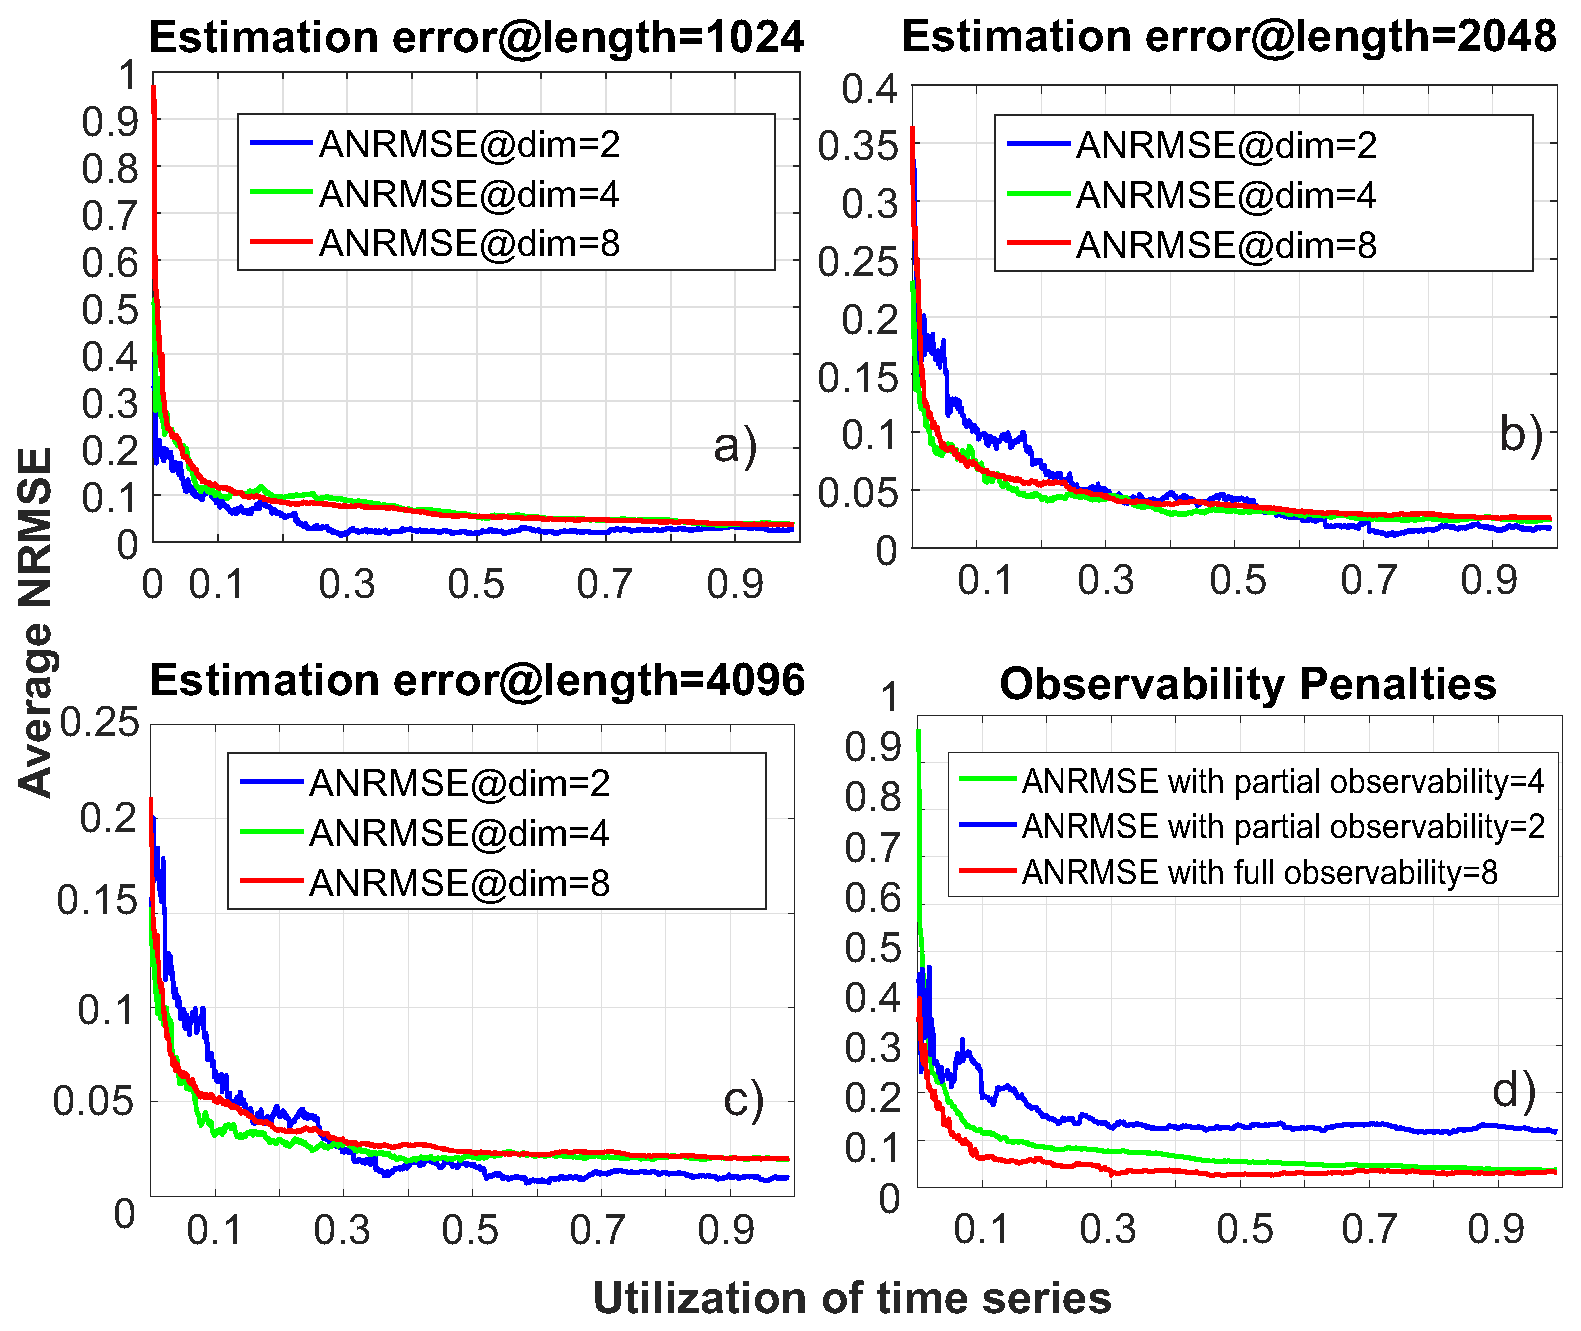
\includegraphics[width=0.95\columnwidth]{effective_algorithm.eps}
\caption{\textbf{The ANRMSE values (a-c) for partial observability of several signal lengths ($1024, 2048, 4096$). d) Partial observability estimating 8-dimensional cross-correlated signals from only $2, 4$ observed channels.} }\label{fig:effective}
\end{figure} 
\begin{figure}%[!]
\centering
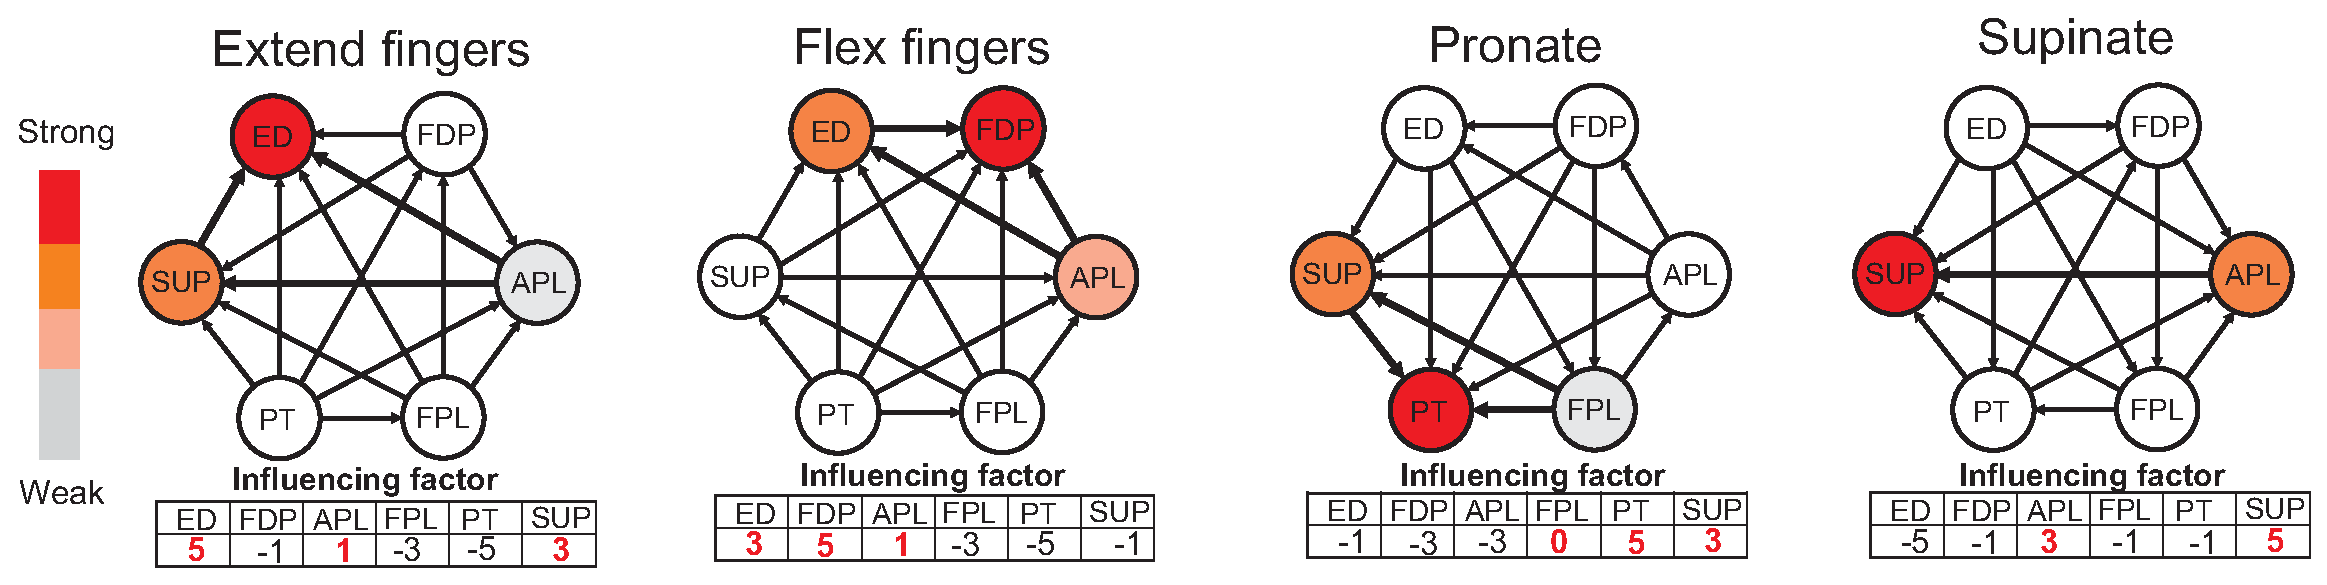
\includegraphics[width=1\columnwidth]{movement.eps}
\caption{\textbf{Fractal connectivity network inferred from 4 different movements. 3 healthy subjects are asked to i) Extend all fingers; ii) Flex all fingers at a consistent strength for 10 seconds or iii) Pronate forearm; iv) Supinate forearm in the experiments. } }\label{fig:movement}
\end{figure}
\begin{figure}%[!]
\centering
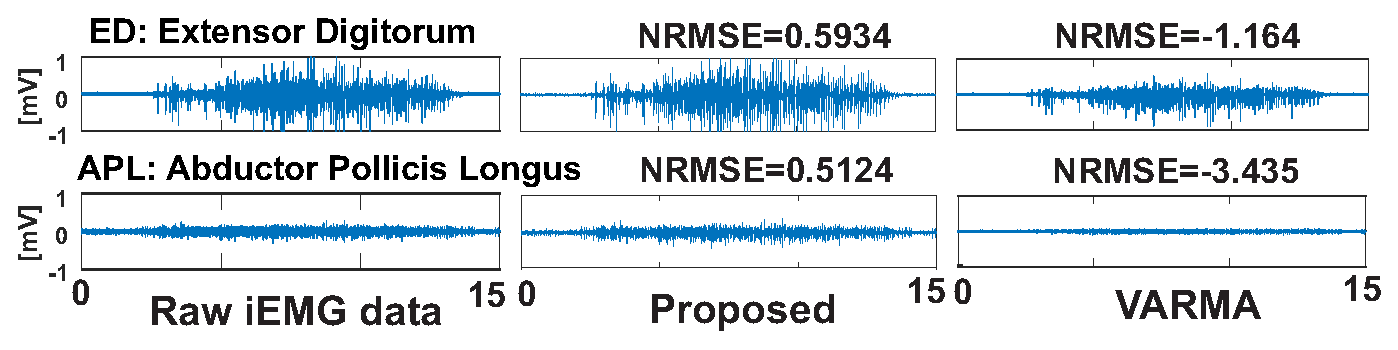
\includegraphics[width=1.0\columnwidth]{comparison_2.eps}
\caption{\textbf{Comparison of first-order model-fitting to 2-channel  (ED and APL) raw iEMG data collected from subject 3 under finger extension} }\label{fig:comparison}
\end{figure}
One major challenge for the design of a CPS approach to BMBI is represented by the need to enable a cyber platform that is able to work with the real-time measurements, identify in real time a compact (few parameters) yet expressive mathematical model and rely on efficient parameter estimation algorithms (determines the mathematical model describing the CPS dynamics from minimum number of samples). This calls for robust and fast algorithms that work with short time series and consistently show good accuracy and fidelity compared to real-time measurements. To justify our proposed framework, we first measure the accuracy of the proposed mathematical identification algorithm in relation to the number of (observed) samples. Then, we show the importance of capturing the spatio-temporal interdependencies of BMBI activities by measuring the deviation in the estimated parameters for two cases: (\textit{i}) The parameters of the model when all the time series are given / observed; (\textit{ii}) The parameters of the model when only a subset of time series are considered.

To investigate the accuracy of the STF modeling framework, we first simulate the proposed model with random choice of $A(L)$ matrix and fractal differencing matrix $D^{\alpha}(L)$ under different signal cardinality (i.e., considering 2, 4 and 8 time series). For each experimental investigation that considers a specific number of time series, we generate 1000 time series of different lengths (i.e., 1024, 2048 and 4096, respectively) and measure the average normalized root mean square error (ANRMSE) between the true and identified parameters as a function of considered number of samples from the initial time series. ANRMSE is calculated as $E[1-\frac{\| \textbf{x}_{ref}-\textbf{x} \|}{\|\textbf{x}_{ref}-E[\textbf{x}_{ref}]\|}]$.

 To obtain the ANRMSE values in Figure \ref{fig:effective}.(a-c), we perform $10^{5}$ experiments for each choice of the number of considered time series, number of considered samples and length of the time series. Simply speaking, we aim to exploit the signals fractality and find the minimum number of samples that would lead to a good model with good accuracy (i.e., the ANRMSE is smaller than a threshold). This would help the CPS to build confidence about the model as the samples are recorded. \\ 
\indent As shown in Figure\ref{fig:effective}.(a-c), the ANRMSE exhibits a phase transition from negligible to noticeable errors as a function of the number of considered samples. For instance, we could use only 30$\%$ of the recordings to learn a good CPS model. In other words, considering only some information about the state-space dynamics represented by the time series (i.e, 10$\%$ or 30$\%$ of the total time series length) the ANRMSE remains almost the same to the case in which more and more samples are included in the identification problem and contributing to higher computational complexity. This can translate into smaller model identification latency and power savings. \\
\indent For many CPS applications, it is important not only to identify a mathematical model with good accuracy from minimum number of samples, but also to be able to retrieve a good model of the system when only a subset of state variables are observed (e.g., reduced order model). In order to study this problem, we consider that from a number of time series  we only know a subset and identify a mathematical model of the form in equation (\ref{eq:backward}). More precisely, we first simulate the proposed model under a cross-dependent model of 8 time series with length of 1024 and generating 1000 trajectories. Then we perform the parameter estimation assuming we only have partial observability (i.e, only consider) to $2$ and $4$ channels from all 8. The ANRMSE values  are reported  in Figure \ref{fig:effective}.(d) as a function of the number of considered samples. As shown in Figure \ref{fig:effective}.(d), when only 4 channels of an 8-dimensional signal representation are observed, the estimation error almost remain the same compared to the case with full observability. It is also noticed that ANRMSE values of the estimated parameters increase noticeably when only two time series out of 8 cross-correlated time series are considered. This implies the failure to model a complex process involving multiple participating entitles (e.g., the cerebral-muscular activities consisting of multiple functional muscles and neurons) and consider sufficient state-variables will lead to model misfitting and biased implication of how these entities are dependent and/or correlated (e.g., the contribution of some muscles in certain movement might be underestimated or overestimated).  
\subsection{Model Validation in Realistic Clinical Experiments}
To investigate the benefits of our model, we compared the goodness-of-fit (GoF) provided by our model and the extensively utilized VARMA model with order $p=1$ when applied to the raw iEMG signals of 6 channels collected from 3 subjects doing different movements. The GoF is quantified in terms of normalized root mean square error (NRMSE) computed for each channel for the two models and averaged over 3 subjects (see Table \ref{tb:fit}). NRMSE is a measure of how well a model fits to the data ranging from $-\infty$ (worst) to $1$ (best). To better illustrate the capability of our fractal modeling approach, Figure  \ref{fig:comparison} summarizes for 2 channels (namely ED and APL when doing finger extension) the comparison between: \textit{i}) First column represents the raw iEMG signals, \textit{ii}) second column denotes the time series generated by our fractal model, and \textit{iii}) third column shows the time series generated by VARMA. As one can notice, VARMA model fits poorly to the raw data with negative NRMSE values. In contrast, our fractal model fits better with NRMSE values over 0.5 for all channels. Table \ref{tb:fit} gives a comprehensive overview of the comparison across all 6 channels from 4 movements. The results consistently show the proposed model gives better fitting over VARMA model. Consequently, our fractal model captures better than VARMA not only the long-range memory of the signals, but also the \textit{cross-dependencies} between signals. Taken together, these results show that modeling fractality can significantly improve not only the GoF of the mathematical model opening the avenue for endowing the CPS with built-in intelligence, but also can lead to a better understanding of fractal properties expressed by biological systems and develop new more efficient control strategies. 
\begin{table}[t]
\center
\caption{Average goodness-of-fit in NRMSE(-inf: worst ; 1 : best)}\label{tb:fit}
\begin{tabular}{|c|c|c|c|c|c|c|c|c|} \hline
\multirow{2}{*}{Channel} & \multicolumn{2}{|c|}{Extend} & \multicolumn{2}{|c|}{Flex} & \multicolumn{2}{|c|}{Pronate} & \multicolumn{2}{|c|}{Supinate} \\
\cline{2-9}
& VA & Frac & VA & Frac & VA & Frac & VA & Frac \\
\hline
ED & -1.2 & 0.52 & -0.86 & 0.47 & -0.15 & 0.30 & -0.65  & 0.46\\
\hline
FDP  & -2.4 & 0.57 & -0.17 & 0.47 & -1.4 & 0.49 & -3.3 & 0.58\\
\hline
APL  & -3.6 & 0.59 & -0.22 & 0.32 & -0.61 & 0.45 & -0.44  & 0.40 \\
\hline
FPL  & -2.5 & 0.55& -1.2 & 0.51 & -9.3 & 0.56 & -2.3  & 0.52\\
\hline
PT  &  -5.9 & 0.59 & -1.8 & 0.54 & -1.0 & 0.50 & -6.2)  & 0.58\\
\hline
SUP  &  -2.7 & 0.57 & -0.13 & 0.25 & -0.33 & 0.36 & -0.37  & 0.55\\
\hline
\end{tabular}
\end{table}
\vskip -2mm
\subsection{Statistical Analysis of Fractal Connectivity}
Fitting the proposed model well to the real neuromuscular processes leads us to several follow-up research directions: i) How can we infer correlations between different participating entities (e.g., different muscles) jointly involved? ii) How can we statistically associate such correlations to specific movements from different subjects in multiple trials to reliably extract patterns? To answer these questions, we exploit the interdependency matrix $A(L)$ and construct the \textit{connectivity network} for pattern recognition. More precisely, we construct the directed graph $G$ from the $A(L)$ coefficients by comparing the off-diagonal coefficients in the symmetric position $(i,j)$ and $(j,i)$ of the matrix with a predefined threshold and drawing directed edge from $j$ to $i$ if muscle $j$ exerts much greater influence on $i$. To deal with variabilities and present reliable patterns, for each connection in $G$, the estimated $A(L)$ coefficients are used to perform a t-test with the null hypothesis that the coefficients come from a distribution with a zero mean (i.e., different muscles are weakly correlated or uncorrelated if no movements are performed). With significance $\alpha=0.05$, the connectivity network is then constructed by including all statistically significant connections, i.e., connections whose $p$-values are smaller than $\alpha$. The resulting connectivity graph for different movements are plotted in Figure \ref{fig:movement}. We quantify the influencing factor $f$ as the difference between the \textit{in}-degree and \textit{out}-degree of a given node. A bigger $f$ is associated with the muscle that is more active in corresponding movement and needs collective assistance from other muscles. The one with biggest $f$ is the dominant muscle in a movement. As one can see from Figure \ref{fig:movement}, our fractal model captures accurately the major dominant muscles involved in all 4 movements and shows consistency with the clinical and anatomical observations \cite{Henry} .
\vskip -7mm
\section{Summary}
In this work, we propose a data-driven fractal mathematical model capable of modeling multi-dimensional cross-dependent BMBI processes with long term dependencies. We justify our model through realistic clinical experiments measuring multi-channel iEMG signals of different natural forearm movements. The comparison between the well-known VARMA and our fractal model shows that our model gives a better fit throughout the experiments. We also statistically infer the fractal connectivity network from the fitted model and show agreement with anatomical observations which lays the foundation for prediction and control of BMBI.
\chapter{Minimum Number of Sensors to Ensure Observability of Physical Systems: Case Studies}
\label{cha:ch4}

Advances in wearable technology allow us to measure all sorts of physiological signals. Fitbit is probably the most familiar to the public in general. It measures data such as the number of steps per day, quality of sleep, steps climbed, and other personal metrics; and  Emotiv is a company that  develops brain-computer interfaces based on electroencephalography (EEG) technology. Nonetheless, these and other technologies are still in their infancy, and far from allowing to predict a cardiac arrest or the beginning of an epileptic seizure. The benefits generated by such capability are expected to revolutionize healthcare, in the sense that it will allow an impairment with a smartphone via wireless or bluetooth, capable of performing an emergency call, or stimulate locally certain points of the human body to mitigate the effects that follow each occurrences. 

Towards that auspicious future, we propose to explore a class of models that will enable the characterization of certain physiological signal dynamics, and allow us to retrieve the overall dynamics associated with certain technologies by only considering a subset of its signals. These models rely on the assumption that acquired signals of the same physiological phenomena have \textit{spatial-temporal properties} that can be captured by the model. This is the case for the electrocardiogram (ECG) signal that records the electrical voltages generated by the heart over a period of time, using electrodes placed across the patient's body: limbs and chest. Commonly, there are between twelve and sixteen ECG electrodes placed on the surface of the patient's body. These sensors capture the potential differences between electrodes that arise from heart-muscle depolarization during each cardiac cycle, measured from different angles in a frame whose heart sets the origin~\cite{hall2015guyton}. This emphasizes the \textit{spatial} and \textit{temporal interdependence} between physiological processes. Further, Fitbit sensor matches one of the leads locations, so one could wonder if it would suffice to predict abnormal cardiac activity, see Figure~\ref{fig:fitbit}. 

\begin{figure}[htb]
\centering
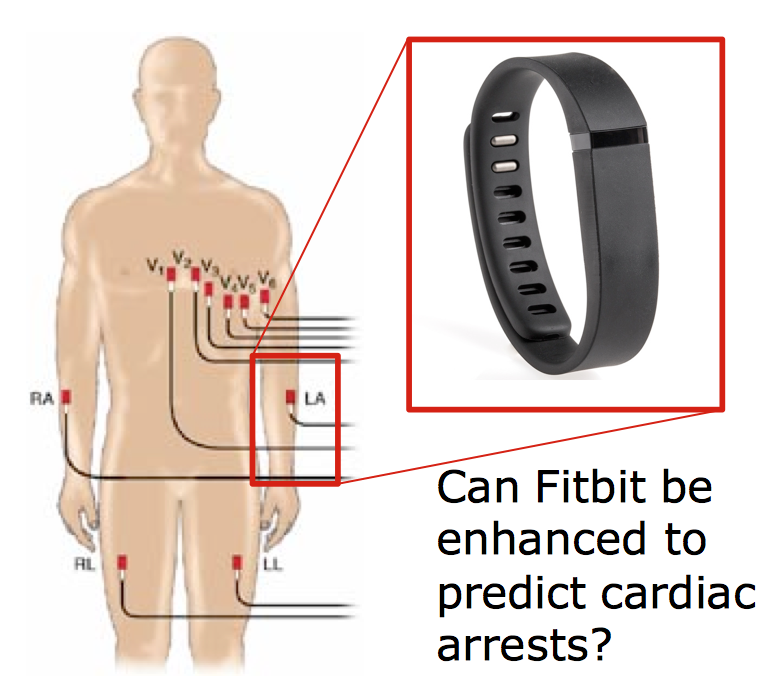
\includegraphics[width=0.50\columnwidth]{fitbit.png}
\caption{\textbf{Can the Fitbit sensor be used to retrieve the overall activity of the remaining sensors, hence, assess if one is about to have a cardiac arrest?}}\label{fig:fitbit}
\vskip -2mm
\end{figure}  

Similarly, the EEG sensors measure electrical potentials (brain waves) resulting from ionic current within the neurons of the brain. Due to the nature of the electrodes used, different sensors may collect data associated with the same activity, and, thus, capturing \textit{interdependent temporal} and \textit{spatial} signals. The frequency of the brain waves recorded from the surface of the scalp can range from once per few seconds to more than 50Hz. The aspect of these waves is dependent on the activity of the correspondent cerebral cortex being acquired, and they can change drastically between states of wakefullness, sleep, coma or in brain diseases such as epilepsy~\cite{hall2015guyton}. Finally,  an electromyography (EMG) signal detects the electrical potential generated by the skeletal muscle cells when these cells are electrically or neurologically activated, hence, resulting in a technique for evaluating and recording the electrical activity produced by skeletal muscles. These signals can then contain dynamical fingerprints that are associated with a configuration of muscle activation, leading to the execution of a specific task. Once again, due to the interdependence of the different biological systems (muscles) in the human body, it is easy to understand that the \textit{spatial} and \textit{temporal dependence} is present. Furthermore, these signals can be analyzed to detect and predict medical abnormalities, activation level, or recruitment order, or to analyze the biomechanics of human or animal movement. 

Unlike current mathematical modeling approaches that rely on memoryless assumptions, the statistical analysis of physiological processes (ECG, EEG, blood glucose) demonstrates that they possess significant degree of long-range memory and fractality. In particular, numerous recent studies show that physiological processes can be more accurately modeled via \emph{fractal order dynamical systems}~\cite{moon1992chaotic,piramideCortexFractal,surveyFractalNeuro,ecgFractal,Thurner2003511}.  Nonetheless, these efforts have either only demonstrated that the statistics of the physiological dynamics is of fractal nature (e.g., the autocorrelation function or the power spectrum exhibit a power law behavior) or only accounted for the temporal dependence of the signals (e.g., demonstrating that there is some form of persistence in time between changes in the magnitude of the physiological process). Subsequently, the spatial dependence existing between various physiological processes cannot be leveraged to obtain information about the signals that are not being directly measured. 

To overcome these limitations, we propose to use \textbf{coupled discrete-time fractal order dynamical systems} (CDFODS) to capture the spatial-temporal characteristics existing between physiological processes. Further, if we aim to retrieve the state of the system from the measurements alone, commonly referred to as \emph{static observability},  the solvability of a set of $p$ measurements equations to recover an $n-$dimensional parameter is required, hence, requiring at least as many measurements as the number of unknowns, $p\ge n$, in general. In addition, if the processes are not spatially dependent, when the sensing technology only accesses a state variable at any given time, then such conditions are not possible to satisfy.  Subsequently, this model allows us to retrieve all its states from the collected data obtained from a small subcollection and the model. This property is commonly referred to as \emph{observability} of the system, and the system (i.e., dynamics and sensing capabilities) that possesses it are referred to as being \emph{observable}~\cite{fracOrderdiscrete} -- see Section~\ref{prelim} for details. Furthermore, in this paper, we propose to extend the use of submodularity tools to find the minimum number of sensors in the CDFODS context that, to the best of our knowledge, has not yet been previously explored. 

Submodular functions are used across multiple fields of science, for instance, mathematics, economics,  circuit theory, operation research and machine learning~\cite{BachSurvey,Edmonds,Lovasz1983,Schrijver}. In particular, examples of machine learning applications include static sensor selection~\cite{KrauseGuestrinInfoGather,KrauseGuestrinSensorPlace} where a dynamic model is not explicitly considered; natural language processing~\cite{kirchhoff}; robotics applications~\cite{atanasov2015a,MeliouKGH07}; and  spatio-temporal processes modeled as linear-time-invariant models under uncertainty~\cite{aiStats}, just to name a few.  The problem of determining the minimum number of sensors to ensure observability in linear-time invariant systems has been explored in~\cite{MinControlProb}, and its optimal solutions in~\cite{PequitoJ4}. In addition, we notice that the previous solutions~\cite{MinControlProb,PequitoJ4} considered the continuous-time integer (non-fractional) order systems. It is also important to notice that although~\cite{MinControlProb,PequitoJ4} propose approximations that resemble the greedy algorithms known to approximate those whose objective are given by a submodular function,  they do not explicitly use these notions as we propose in this paper. 

The contributions of this paper are fourfold: (i) we explain how to cast the evolution of several spatial-temporal-related physiological signals into a CDFODS framework; (ii) we show that the problem of determining the minimum number of sensors required to ensure observability of CDFODS is NP-hard; (iii) we propose to use submodularity theory to approximate the results, which yields optimality guarantees; and  (iv) we show its application in the context of three physiological signals, i.e., EEG, ECG and EMG.

The remaining of the paper is organized as follows: Section~\ref{probStat} introduces the CDFODS and the mathematical formulation of the problem to determine the minimum number of sensors to obtain an observable system. In Section~\ref{prelim}, we revisit some of the properties of the CDFODS and submodularity theory. The theoretical  results of this paper are presented in Section~\ref{mainResults}, whereas in Section~\ref{illustExam} we study several applications of the proposed framework.


\section{Problem Statement}\label{probStat}
Consider a model dynamics described by a linear discrete-time fractional-order system as follows


%\begin{equation}
%\Delta^{\boldsymbol{\alpha}}x_{k+1}=\left[ \begin{array}{c}
%\Delta^{\alpha_1} x^1_{k+1}\\
%\Delta^{\alpha_2} x^2_{k+1}\\
%\vdots\\
%\Delta^{\alpha_n} x^n_{k+1}
%\end{array}
%\right]=\sum\limits_{j=0}^{k+1}A_j x_{k},\label{fracDyn}
%\end{equation}


\begin{equation}
\label{fracDyn}
\left[ \begin{array}{cccc}
D^{\alpha_1}&&&\\
%&D^{\alpha_2}&&\\
&&\ddots &\\
&&& D^{\alpha_n}
\end{array}
\right]x[k+1]=Ax[k],  
\end{equation}
where $k=0,1,\ldots, T$; $\alpha_i\in\mathbb{R}^{+}$ for $i=1,\ldots,n$; and $D^{\alpha_i}$ is the discretized fractional-order operator~\cite{fracOrderdiscrete}, and $x[0]=x_0\in\mathbb{R}^n$ the initial condition. Further, for brevity, we refer to the dynamics in~\eqref{fracDyn} as $\mathcal F(A;\boldsymbol{\alpha},K)$, where $\boldsymbol{\alpha}=(\alpha_1,\ldots, \alpha_n)$. In addition, assume that a collection of sensors is deployed to collect data about the state of the system. If a sensor is able to capture a linear combination of state variables, then the collection of sensors measurements can be represented as follows:
\begin{equation}
y[k]=Cx[k],
\label{outputGenericDiscrete}
\end{equation}
where $C$ is a matrix with appropriate dimensions encoding the linear combination. In the static case, i.e., when we aim to retrieve the state of the system from the measurements alone, (static) observability requires the solvability of a set of $p$ measurements equations to recover an $n-$dimensional parameter, hence, requiring at least as many measurements as the number of unknowns, $p\ge n$, in general. Alternatively, as often occurs in several setups, the sensor captures only a state variable (instead of a linear combination of these), i.e., the collection of measurements is given by
\begin{equation}
y[k]=\mathbb{I}_n^{\mathcal J}x[k],
\label{outputDiscrete}
\end{equation}
where $\mathcal J$ denotes the indices of the state  variables being measured, and $\mathbb{I}^{\mathcal J}_{n}$ denotes the matrix that consists of the rows of the identity matrix with indices in $\mathcal J$. Hence, no solution exists that retrieves the state variables that are not being measured, when only the collection of measurements is considered.  To overcome the two issues mentioned, we propose to  consider the model that captures the spatial-temporal relationship between the state variables that together with the measurements will enable the retrieval of the state. A system $\mathcal F(A;\boldsymbol{\alpha},K)$ and a collection of measurements~\eqref{outputDiscrete} is said to be (dynamically) \emph{observable} at time $k=0$ if and only if there exists some $T$ such that the state $x_0$ can be uniquely determined from the knowledge of $y_k$ and $\mathcal F(A;\boldsymbol{\alpha},K)$. Subsequently, the goal of this paper is to determine the minimum $\mathcal J$ in~\eqref{outputDiscrete} that, together with $\mathcal F(A;\boldsymbol{\alpha},K)$, ensures observability of the system at time $k=0$. We have the following problem:

  

\textit{Minimum Sensor Placement Problem}


Given $\mathcal F(A;\boldsymbol{\alpha},K)$,  determine the minimum number of dedicated sensors $\mathcal J$  such that
\begin{equation}
\begin{array}{cc}
\arg\min\limits_{\mathcal J\subset \{1,\ldots,n\}} & |\mathcal J|\\
\text{s.t.} & (\mathcal F(A;\boldsymbol{\alpha},K),\mathbb{I}_n^{\mathcal J}) \text{ is observable.}
\end{array}
\label{optProbP2}
\end{equation}
\hfill $\circ$

\begin{figure}[htb]
\centering
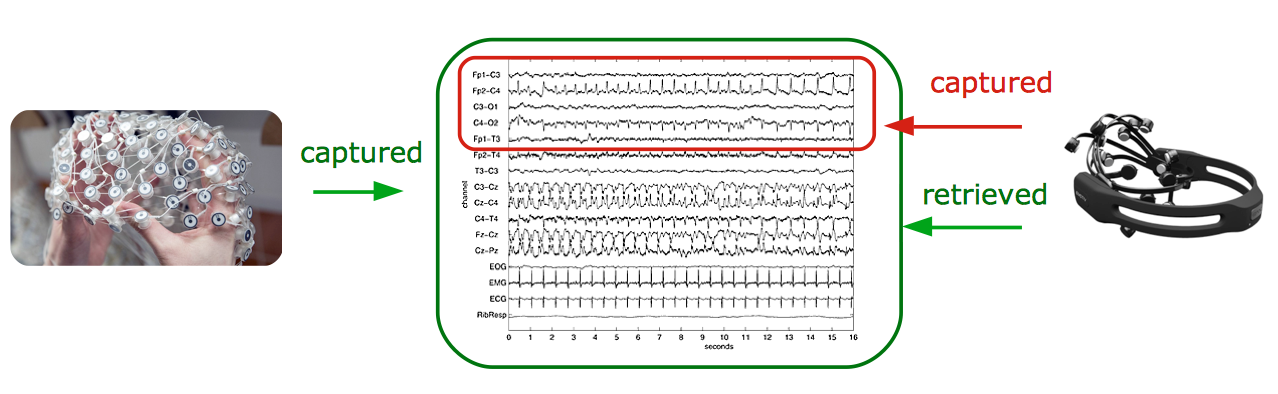
\includegraphics[width=1\columnwidth]{eegCapRec.png}
\caption{\textbf{Are both technologies equivalent?}}\label{fig:EEGCapRec}
\end{figure}

Figure~\ref{fig:EEGCapRec} illustrates one possible application of this problem, i.e., determine if a subcollection of sensors allow to retrieve the overall evolution of  EEG signals. In particular, determining the smallest collection of such sensors will lead to the development of energy efficient EEG wearables.





\section{CDFODS Observability and Submodularity}\label{prelim}

In this section, we first review  some properties of the CDFODS and the characterization of the feasibility space of~\eqref{optProbP2}, followed by a brief recap of submodularity properties. The closed-form to~\eqref{fracDyn} is described as follows.

\begin{lemma}[\cite{fracOrderdiscrete,fracOrderdiscreteJournal}]
The solution to~\eqref{fracDyn} is given by:
\begin{equation}
x[{k+1}]=G_{k+1}x[0],
\label{fracDynSol}
\end{equation}
\noindent where
\[
G_k=\left\{\begin{array}{cl}
\mathbb{I} & \text{for } k=0,\\
\sum\limits_{j=0}^{k-1}A_jG_{k-1-j}& \text{for } k\ge 1,
\end{array}\right.
\]

with $A_0=A$ and $A_j=\text{diag}(${\small$- (-1)^{j+1} \binom{\alpha_1}{j+1},\ldots,$ \\
$- (-1)^{j+1} \binom{\alpha_n}{j+1}$}$)$. Please note that $\alpha$ is a non-integer number and the term $\binom{\alpha}{j} = \frac{\Gamma(\alpha+1)}{\Gamma(j+1)\Gamma(\alpha-j+1)}$ is expressed via the Gamma function: $\Gamma (x) = \int_{0}^{\infty} t^{x-1}e^{-t}dt$ \cite{Baleanu}.\label{LemmaClosedForm}
\hfill $\diamond$
\end{lemma}

Subsequently, consider a sequence of measurements of the closed-form described in Lemma~\ref{LemmaClosedForm}, i.e.,
\begin{align*}
y[1]=Cx[1]=CG_0& x[0], \  y[2]=Cx[2]=CG_1x[0], \notag \\
 &\ldots, \ y[K]=Cx[K]=CG_{K-1}x[0].\notag
\end{align*}

We can rewrite it as
\begin{equation}
y_{0:K}=\underbrace{[(CG_0)^{\intercal} \ (CG_1)^{\intercal} \ \ldots \ (CG_{k-1})^{\intercal}]^{\intercal}}_{\mathcal O_k(\mathcal F(A;\mathbf{\alpha},K),C)}x[0],
\label{evolMeasurements}
\end{equation}
where $y_{0:K}=[y^\intercal_0 \  y^\intercal_1 \ \cdots \ y^\intercal_K]^\intercal$, and the matrix $\mathcal O_k(\mathcal F(A;\mathbf{\alpha},K),C)$ is commonly referred to as \emph{observability matrix}. In order to retrieve $x[0]$, we can first premultiply both hand sides of~\eqref{evolMeasurements} by $\mathcal O^{\intercal}\equiv\mathcal O_k(\mathcal F(A;\mathbf{\alpha},k),C)$, which leads to
\[
\mathcal O^{\intercal}y_{0:K}=\mathcal O^{\intercal}\mathcal Ox[0].
\]
Thus, if $\mathcal O^{\intercal}\mathcal O$ is invertible, then we obtain a closed-form solution to $x[0]$, i.e., 
\begin{equation}
x[0]=(\mathcal O^{\intercal}\mathcal O)^{-1}\mathcal O^{\intercal}y_{0:K}.\label{retrieveDynFracEq}
\end{equation}
As a consequence, we obtain the following results:




\begin{theorem}[\cite{fracOrderdiscrete,fracOrderdiscreteJournal}]
The system described by \eqref{fracDyn} and \eqref{outputGenericDiscrete}  is observable if and only if there exists a finite time $K$ such that $\text{rank } (\mathcal O_K(\mathcal F(A;\mathbf{\alpha},K),C))=n$. \hfill $\diamond$
\label{observabilityDynFrac}
\end{theorem}





\begin{theorem}[\cite{fracOrderdiscrete,fracOrderdiscreteJournal}]
If the system described by \eqref{fracDyn} and \eqref{outputGenericDiscrete}  is observable, then the initial state $x_0$ can be retrieved as in~\eqref{retrieveDynFracEq}.
\hfill $\diamond$
\label{retrieveDynFrac}
\end{theorem}

\begin{remark}
Due to the nature of Theorem~\ref{observabilityDynFrac}, it may occur that a specific set of measurements do not yield observability of a given time $K$. Notwithstanding, it is possible that there exits  $K'>K$ that for the same collection of sensors  such that Theorem~\ref{observabilityDynFrac} holds. In other words, observability implicit considers the tradeoffs between how much data is collected (with the same set of measurements), in particular, the  time allowed to collect data, and the number of sensors  acquiring it. \hfill $\diamond$
\end{remark}


In section 4, we show how the aforementioned characterization of the feasibility space of~\eqref{optProbP2} can be used to obtain its solution. Briefly, we will use a submodular approach. 

Given a finite set $\mathcal V$ with $n$ objects, i.e., $|\mathcal V|=n$, we can define a function $f:2^{\mathcal V}\rightarrow \mathbb{R}^+$ that associates a positive scalar with each subset of $\mathcal V$. This function is said to be \emph{submodular} if it satisfies the so-called \emph{diminishing returns} property, i.e., for all $\mathcal X\subset \mathcal Y$ and $v\notin \mathcal Y$, we must have: $$f(\mathcal X\cup \{v\})-f(\mathcal X)\ge f(\mathcal Y\cup \{v\})-f(\mathcal Y).$$ In other words, the increment by considering a new element in a smaller sized set is at least as high as adding it to a superset of the latter. When $f$ is submodular, one can use greedy algorithms that yield approximate solutions that are at most $33\%$ worse than the optimal solution~\cite{Nemhauser}. These approximation guarantee does not depend on the size of $\mathcal V$ and it provides a worst case scenario that is often not attained; in addition, some improved guarantees are available when submodular functions have additional properties, see~\cite{LinBilmes} for details.

\section{Minimum Sensor Placement}\label{mainResults}

In this section, we present the main results of this paper. More precisely, in Theorem~\ref{complexity} we show our problem to be NP-hard. Notwithstanding, we present an heuristic  Algorithm~\ref{algorithm1} that has polynomial computational complexity, and approximates the original problem with some optimality guarantees, see Theorem~\ref{algorithmApproxResult}. 



\begin{theorem}
The minimum sensor placement problem for CDFODS~\eqref{optProbP2} is NP-hard.\hfill $\diamond$
\label{complexity}
\end{theorem}

\textbf{Proof: }
The proof follows by noticing that there exists a set of coefficients $\mathbf{\alpha}$ that leads to $A_j=\mathbb{I}_n$ for $j=1,\ldots,K$. Therefore,~\eqref{optProbP2} reduces to a linear time-invariant system, and the problem reduces to the minimum observability problem for linear-time invariant systems presented in~\cite{MinControlProb}, that is NP-hard. Thus, because~\eqref{optProbP2} contains (as subclass of problems) one that is NP-hard, it follows that~\eqref{optProbP2} is also NP-hard.\hfill $\blacksquare$






\begin{algorithm}[tb]
   \caption{Heuristic Algorithm to~\eqref{optProbP2}}
   \label{algorithm1}
\begin{algorithmic}
   \STATE {\bfseries Input:} CDFODS $\mathcal F(A;\mathbf{\alpha},K)$;
      \STATE {\bfseries Output:} $\mathcal J^*$  that is an approximate solution to~\eqref{optProbP2};
      \vspace{0.2cm}
      {
   \STATE Initialize $ \mathcal J^*=\emptyset $; 
   \REPEAT
   \STATE Initialize $\Delta r^* = 0$;
   \STATE $r_{0}=\text{rank}(\mathcal O_k(\mathcal F(A;\mathbf{\alpha},K),\mathbb{I}_n^{\mathcal J^*}))$;
   \FOR{$i=1$ {\bfseries to} $n$}
   \STATE $\mathcal J'= \mathcal J^* \cup \{i\}$;
   \STATE $\Delta r(i)=\text{rank}(\mathcal O_k(\mathcal F(A;\mathbf{\alpha},K),\mathbb{I}_n^{\mathcal J'}))-r_{0}$;
   \IF{$\Delta r(i) > \Delta r^* $} 
   \STATE $\Delta r^*=\Delta r(i)$;
   \STATE $i^*=i$;
   \ENDIF
   \ENDFOR
   \IF{$\Delta r^* > 0$} 
   \STATE $\mathcal J^*=\mathcal J^* \cup \{i^*\}$;
   \ENDIF
   \UNTIL{$\Delta r^* = 0$.  } 
   }
\end{algorithmic}
\end{algorithm}

Next, we show that the feasibility space of~\eqref{optProbP2} is given by a constraint, see Theorem~\ref{observabilityDynFrac}, that is submodular.


\begin{lemma}
Given a CDFODS $\mathcal F(A;\mathbf{\alpha},K)$,  the following function $$f(\mathcal J)=\text{rank}(\mathcal O_k(\mathcal F(A;\mathbf{\alpha},K),\mathbb{I}_n^{\mathcal J}))$$ is submodular in $\mathcal J\subset\{1,\ldots, n\}$.
\hfill $\diamond$
\label{submodular}
\end{lemma}

{
\textbf{Proof: } We define $\mathcal V=\{1,2,\ldots,nK\}$  as the set of row vector indices for observability matrix $\mathcal O_k(\mathcal F(A;\mathbf{\alpha},K),\mathbb{I}_n)$. Let $\mathcal V_{\mathcal J_{A}} \subseteq \mathcal V$ be the set of row vector indices for $\mathcal O_k(\mathcal F(A;\mathbf{\alpha},K),\mathbb{I}_n^{\mathcal J_{A}})$, where $\mathcal J_{A}\subset \{1,\ldots,n\}$. Let $r(\mathcal V_{\mathcal J_{A}})$ be the rank of the matrix that contains as rows the row vectors $\{g_{i}\}_{i \in \mathcal V_{\mathcal J_{A}}}$ indexed by $\mathcal V_{\mathcal J_{A}}$. Hence, $r:2^{\mathcal V} \rightarrow \mathbb{Z}^{+}\subset \mathbb{R}^+$ is the rank function of observability matrix and $r(\mathcal V_{\mathcal J_{A}})$ is the cardinality of maximum independent subset of vectors contained within the set of vectors indexed by $\mathcal V_{\mathcal J_{A}}$. Therefore, $r(\mathcal V_{\mathcal J_{A}}) = \text{rank}(\mathcal O_k(\mathcal F(A;\mathbf{\alpha},K),\mathbb{I}_n^{\mathcal J_{A}}))$. 

Now consider two subset $\mathcal V_{\mathcal J_{A}},\mathcal V_{\mathcal J_{B}} \subseteq \mathcal V$. Let $\mathcal I$, $\mathcal I_{\mathcal A\mathcal B}$, $\mathcal I_{\mathcal A}$ be the maximum independent subset of $\mathcal V_{\mathcal J_{A}} \cap \mathcal V_{\mathcal J_{B}}$, $\mathcal V_{\mathcal J_{A}} \cup \mathcal V_{\mathcal J_{B}}$ and $\mathcal V_{\mathcal J_{A}}$, respectively. By definition, we have $\mathcal {I \subseteq I_{A} \subseteq I_{AB}}$. To prove the submodularity of the rank function $r$, we need to show,
\begin{equation}
	r(\mathcal V_{\mathcal J_{A}})+r(\mathcal V_{\mathcal J_{B}}) \geq r(\mathcal V_{\mathcal J_{A}} \cup \mathcal V_{\mathcal J_{B}})+r(\mathcal V_{\mathcal J_{A}} \cap \mathcal V_{\mathcal J_{B}})
\end{equation}
or equivalently,
\begin{equation}
	r(\mathcal V_{\mathcal J_{B}}) \geq \mathcal{|I_{AB}|}-\mathcal {|I_{A}|}+\mathcal{|I|}.
\end{equation}
following the fact that $|\mathcal I |=r(\mathcal V_{\mathcal J_{A}} \cap \mathcal V_{\mathcal J_{B}})$, $\mathcal {|I_{AB}|}=r(\mathcal V_{\mathcal J_{A}} \cup \mathcal V_{\mathcal J_{B}})$ and $\mathcal {|I_{A}|}=r(\mathcal V_{\mathcal J_{A}})$. Observe that $\mathcal{I_{AB}} \cap \mathcal V_{\mathcal J_{B}}$ is also a set of independent vectors  and a subset of $\mathcal V_{\mathcal J_{B}}$. Therefore, we have
\begin{equation}
      r(\mathcal V_{\mathcal J_{B}}) \geq |\mathcal{I_{AB}} \cap V_{\mathcal J_{B}}|,
\end{equation}
and since $\mathcal{I_{AB}} \cap \mathcal V_{\mathcal J_{B}}$ =$\mathcal{I_{AB}}\setminus (\mathcal V_{\mathcal J_{A}}\setminus \mathcal I)$, it follows that
\begin{equation}
      r(V_{\mathcal J_{B}}) \geq \mathcal{|\mathcal{I_{AB}\setminus (V_{J_{A}}\setminus I)}|}=\mathcal{|I_{AB}|}-\mathcal {|I_{A}|}+\mathcal{|I|}.
\end{equation}
Hence, the  function $f(\mathcal J)=r(\mathcal V_{\mathcal J})$  is submodular.
\hfill $\blacksquare$
}

We now consider the minimum sensor placement problem for CDFODS in~\eqref{optProbP2}. Although we showed the problem is NP-hard,  Lemma~\ref{submodular} proves that the rank of the observability matrix is submodular. Thus, the problem can be solved via greedy approach that repeatedly adds a sensor increasing the rank until the conditions in Theorem~1 hold. Algorithm~\ref{algorithm1} implements such approach. Our first step starts with an empty set $\mathcal J^*$ which contains the index of column vectors to be added to $C$.  The algorithm will tentatively add one index to check if the rank of the observability matrix increases and saves the one that contributes more during one iteration. The loop repeats until the rank stops increasing, case in which the algorithm will stop with~$\mathcal J^*$.
\begin{theorem}
Algorithm~\ref{algorithm1} approximates the minimum observability problem for discrete-time fractional-order systems~\eqref{optProbP2} in polynomial-time, i.e., with computational complexity~$\mathcal O(n^{5})$. Further, it achieves a solution that is at most $33\%$ worse than the optimal solution.\hfill $\diamond$
\label{algorithmApproxResult}
\end{theorem}

{
\textbf{Proof: } Algorithm~\ref{algorithm1} is a greedy method that progressively picks up the index of a column vector from the identity matrix and adds it to $\mathcal J$ such that the maximal increase of rank for observability matrix $O_k(\mathcal F(A;\mathbf{\alpha},K),\mathbb{I}_n^{\mathcal J})$ in each iteration is obtained. The algorithm will terminate when no further increase is possible. Notice that the outer loop will at most be executed $n$ times as $r(CG_{0})=r(\mathbb{I}_n^{\mathcal J})=|J|$, offering a lower bound for the rank of the observability matrix. No more than $n$ indices will be added to $\mathcal J$ until the row rank of $O_k(\mathcal F(A;\mathbf{\alpha},K),\mathbb{I}_n^{\mathcal J})$ is $n$ or the system modeled by \eqref{fracDyn} is observable. In each iteration, the algorithm will loop over all $n$ indices and check their possible contribution to the rank increase when the corresponding column vector is added to $\mathbb{I}_n^{\mathcal J}$. Therefore, any operation in the algorithm will be performed no more than $n^2$ times before rank of observability matrix is full-rank. Since the rank verification of the observability matrix is the most expensive operation and the remaining operations (i.e., comparison, set union and assignment) all have the time complexity of $\mathcal O(1)$, the cost of the rank verification operation determines the overall time complexity of the algorithm. Checking the rank of a matrix can be done using rank-revealing QR factorization with a complexity of $\mathcal O(n^3)$. Therefore, the overall complexity of the algorithm is $\mathcal O(n^5)$. In addition, this algorithm is the greedy algorithm used for submodularity function. Hence, because the objective function considered is submodular by Lemma~\ref{submodular} it follows that the algorithm ensures similar optimality guarantees. In particular, it achieves values within the mentioned bound.
\hfill $\blacksquare$
}
\begin{figure}[tb]
\centering
\includegraphics[width=0.90\columnwidth]{muscles.pdf}
\caption{\textbf{Sensor distribution in the 6-channel iEMG signal clinical measurement experiment. The sensors in blue represent the minimal deployment of sensors that ensure the global dynamics of iEMG in all 6 muscles can be retrieved. The sensors in grey represent the unused sensors while the muscular activity at where the sensor in red is located is simulated based on the identified fractional order system.}}\label{fig:EMG_exp}
\vskip -6mm
\end{figure}   
\section{Simulation Results}\label{illustExam}
%The following examples show applications of the proposed model for determining the minimum set of signals to characterize the overall dynamics of multiple physiological signals.
\textit{A case-study investigation of EMG signals}:

We analyze the intramuscular EMG (iEMG) signals from clinical experiment to compare muscle contractions of transradial amputees to those of non-amputated subjects. All subjects are asked to perform forearm movements. The iEMG signals are recorded at different sites of the forearm muscles as shown in Figure \ref{fig:EMG_exp}: (1) extensor digitorum (ED); (2) flexor digitorum profundus (FDP); (3) abductor pollicis longus (APL); (4) flexor pollicis longus (FPL); (5) pronator teres (PT); and (6) supinator (SUP). Each subject is inserted with fine wire electrodes for measurement purpose. Subjects are asked to relax 6 seconds, then do the finger flexion at a consistent strength for 10 seconds. The entire process is repeated twice. The ADInstruments data acquisition system sampled the iEMG at 4 KHz after applying a 2 KHz low pass filter, and a 10 Hz high pass filter to minimize any motion artifacts from electrodes or leads.
 As an example, we consider iEMG signals measured when the subject 3 is performing the finger flexion at a constant strength. We use identification techniques to estimate the fractional-order parameters $(A,\mathbf{\alpha})$, that account for the spacial-temporal characterization of the signals. More specifically, the coupling matrix captures the spatial dependencies among different motor muscles involved in the forearm movement and the fractional order exponents of different iEMG channels lie in $[-0.14, 0.19]$ that support the nature of fractional dynamics.
 
 Based on the identified system $\mathcal F(A;\mathbb{\alpha},K)$, we perform the greedy method proposed in Algorithm~\ref{algorithm1} to retrieve a small collection of sensors required such that the fractional order system is observable. In Figure \ref{fig:EMG_exp}, we depict in blue the identified sensors that ensure retrieval of initial states for unobserved muscular activities. In Figure \ref{fig:exp_result}(a-1), we report the retrieved initial states over all 6 sensing channels compared against the actual measurements. These states were recovered using~\eqref{retrieveDynFracEq}, when the sensors ED, FDP and APL are considered. In particular, we notice that we were able to successfully recover the initial states of sensors SUP, PT and FPL. To show the capability of retrieving the initial states, we simulate the muscular dynamics over first 10-second session of finger flexion at FPL based on the retrieved system states and the inferred innovation series from our estimation. To give an intuition, we show the comparison between the signal recorded and the simulated activities in Figure \ref{fig:exp_result}(a-2). As we can see from the figure, the simulated dynamics at the non-measured FPL channel fits well to the actually recorded muscular activities, thus, validating the capability of the proposed algorithm to recover global dynamics in the iEMG experiment.
 
 To explore the influence of the length of the time-series, i.e., the number of measurements samples collected, on the accuracy of retrieved global dynamics, we measured the accumulated errors of retrieved system initial states, i.e.,  sum of the deviation from the actual recordings over all sensing channels, and show in Figure \ref{fig:observ_emg}. An important observation is that the increase in number of sensors deployed will help reduce the estimation errors, that are namely  due to approximation errors and small weights in the coupling between some of the sensors' signals. Similar conclusions can be achieved when we observe the physiological process for a longer period of  time, given a fixed number of sensors used.  However, there exists a phase-change phenomenon as the number of sensors used decreases: one can always retrieve the system's initial states with similar accuracy when at least 3 sensors are used, and enough observations are made. However, there is a jump in the accumulated errors that persists over observation horizon if less than 3 sensors are deployed, which suggests the existence of a lower bound for the number of sensors to retrieve global dynamics (i.e., minimal observability), as predicted by the theoretical setting explored in this paper.
 \begin{figure}[htb]
\centering
\includegraphics[width=0.85\columnwidth]{observ_emg.pdf}
\caption{\textbf{The figure shows the accumulated errors in retrieved system's initial states change as a function of the number of used sensors and the observation length. The increase in number of sensor deployed provides information gain that leads to the decrease in overall reduced deviation of states retrieved compared to the actual measurements.}}\label{fig:observ_emg}
\vskip -4mm
\end{figure} 
\begin{figure}[htb]
\centering
\includegraphics[width=1\columnwidth]{overall.pdf}
\caption{\textbf{ The retrieved initial states of the system using \eqref{retrieveDynFracEq} across different signals are presented in the top row. We show the simulated states evolution of sensors that were not considered in the experiments and compare them with actual measurements at these sensors. In the first column, Figure \ref{fig:exp_result}(a-1) shows The initial states of unused sensors are recovered by the proposed algorithm based on the measurements from minimal subset of sensors (ED,APL and FDP). In Figure \ref{fig:exp_result}(a-2), the simulated data based on the retrieved initial states at unused FPL-sensor is compared against the actual measurements during first 0.4 second of finger flexion. Similarly, Figure \ref{fig:exp_result}(b) and Figure \ref{fig:exp_result}(c) show the initial states retrieved for unused sensors and the simulated dynamics at one of these sensors during the experiments of EEG and ECG, respectively.}}\label{fig:exp_result}
\vskip -5mm
\end{figure}  
 
\textit{A case-study investigation of EEG signals}:
\begin{figure}[htb]
\centering
\includegraphics[width=0.8\columnwidth]{EEG_setup.pdf}
\caption{\textbf{The 64-channel geodesic sensor distribution for measurement of EEG. The sensors in blue represent the minimum number of sensors and their deployment to guarantee that the CDFODS in ~\eqref{fracDyn}, whose states correspond to the channel measurements,  is observable. The sensor in red is used as a sanity check on the evolution of  the identified CDFODS. The results are compared against the recorded activity in Figure \ref{fig:exp_result}.(b-2) }}\label{fig:EEG_exp}
\vskip -2mm
\end{figure} 

To explore the minimal observability of a neural system, we apply the proposed algorithm to a 64-channel electroencephalogram data set which records the brain activity of 109 subjects when they are performing motor and imagery tasks. In the experiment, each subject sits in front of a screen where targets might appear at the right/left/top/bottom side of the screen. Upon noticing the target, each subject is asked to open and close the corresponding fists or feet as a function of where the target appears. Each individual performed 14 experimental runs consisting of one minute with eyes open, one minute with eyes closed, and three two-minute runs of interacting with the target. The data set is collected by BCI2000 system with a sampling rate of 160Hz \cite{Physio_EEG, Physio_EEG_2}.

Following the similar experimental settings to that of the iEMG, spatial-temporal parameters were estimated;in particular, the fractal order exponents range from 0.34 to 1.04. Then, using the estimated model, we used Algorithm~\ref{algorithm1} to obtain the $\mathcal F(A;\mathbf{\alpha},K)$ and sensors placement to achievie system's observability. The minimal set of sensors and their deployment are reported in Figure \ref{fig:EEG_exp} and  and depicted in blue. More specifically, 30 out of 64 sensors are required to ensure observability. In addition, we retrieved the system's initial states of all 64 EEG channels by applying equation \eqref{retrieveDynFracEq} and as presented  in Figure~\ref{fig:exp_result}(b-1). Furthermore, as illustrated in Figure~\ref{fig:exp_result}(b-2), the recovered neural system's initial states follow closely the actual measurements. In particular, we simulate the neural dynamics at a distant PO$_{8}$ channel whose retrieved initial state differs by less than $4\%$ from recorded value, and compare the model response with the actual EEG recordings. 
\begin{figure}[htb]
\centering
\includegraphics[width=0.85\columnwidth]{observ_eeg.pdf}
\caption{\textbf{The accumulated errors of the retrieved neural system's initial states over 64 channels change over observation horizon. A phase-change phenomenon is shown when number of sensors deployed drops from 16 to 8 where the errors do not decrease as more observations are made.}}\label{fig:observ_eeg}
\vskip -1mm
\end{figure} 

In what follows, we performed an experiment to check how the length of observations affects the accuracy of the retrieved states under different neural sensor settings. The results are reported in Figure \ref{fig:observ_ecg}, and, as expected, it is shown that the errors of the retrieved states decrease as  we make observations on the system dynamics for a longer period of time given a fixed set of sensors selected, and when we choose more sensors given a fixed length of observations. The similar phase-change phenomenon described for the same experiment using EMG, is also noticed when we use less than 16 sensors in which the accuracy does not improve at the expense of observation length. Further, there exists a sudden increase of errors over all sensing channel when the number of sensors we use drop from 16 to 8.


\textit{A case-study investigation of ECG signals}:
\begin{figure}[!htb]
\centering
\includegraphics[width=0.94\columnwidth]{setup_ecg.pdf}
\caption{\textbf{The deployment of 12-lead ECG system used in the experiment is shown. The sensors in blue (I and II) is the identified  minimal subset of sensors to ensure the observability of the fractional order system. We simulate the cardiac activity at aV$_{\text{R}}$ given the identified fractional order system. }}\label{fig:ECG_exp}
\vskip -4mm
\end{figure}   
\begin{figure}[!htb]
\centering
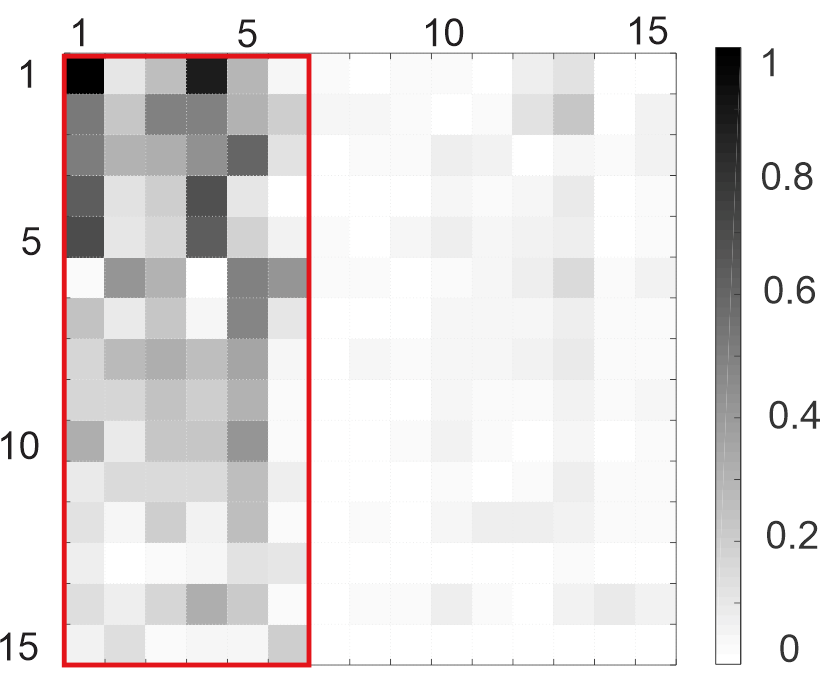
\includegraphics[width=0.85\columnwidth]{sparsity_ecg.png}
\caption{\textbf{The coefficients colormap of spatio-coupling matrix $A$. The distribution of normalized coefficients shows a subset of channels plays dominant roles in the cardiac dynamics. }}\label{fig:ECG_colormap}
\vskip -6mm
\end{figure}  

To verify the efficacy of our theoretical analysis results, we also consider the application of the algorithm to analyze the electrocardiogram (ECG). The raw clinical ECG data was extracted from the PTB diagnostic ECG database~\cite{goldberger2000physiobank}. Data on $52$ healthy subjects ($13$ women, age $48 \pm 19$ and $39$ men, age $42 \pm 14$) was obtained by the National Metrology Institute of Germany. Each subject's record includes 15 different signals simultaneously acquired: the conventional 12-lead (I, II, III, aV$_{\text{R}}$, aV$_{\text{L}}$, aV$_{\text{F}}$, V$_{\text{1}}$, V$_{\text{2}}$, V$_{\text{3}}$, V$_{\text{4}}$, V$_{\text{5}}$, and V$_{\text{6}}$) and 3 Frank orthogonal leads (V$_{\text{X}}$, V$_{\text{Y}}$, and V$_{\text{Z}}$). Each signal is digitalized at 1000Hz, with a signal bandwith of 0Hz to 1KHz and with 1 uV LSB resolution~\cite{Bousseljot1995}. As an example, we choose the ECG signal from the subject S0010 from the data set during a 39-second measurement session. Similarly, we first obtain the estimate of $\{\alpha_{j}\}$ that corresponds to the fractional order derivative in equation \eqref{fracDyn} and the spatio-coupling matrix $A$. Based on the identified system, the greedy algorithm shows we do not need more than two sensors(i.e., $I$ and $II$) to retrieve the dynamics of all 15-channel cardiac activities. We show the recovered system states using the observation from only two sensors in blue in Figure \ref{fig:ECG_exp}.(c-1). An important observation is that the obtained deployment of sensors aligns with the pattern distribution of coefficients in the coupling matrix $A$, see Figure \ref{fig:ECG_colormap}. A subset of channels plays the dominant role in the cardiac dynamics and these channels themselves are tightly coupled such that we can retrieve global dynamics by the observations made upon a subset of them. This is verified by the output of algorithm and validated during our simulation to generate the system states evolution at aV$_{\text{R}}$ as shown in Figure \ref{fig:exp_result}.(c-2). The simulated model response is strongly coherent with actual measurement. We set up the similar experiment to show the relation between the observation length and number of sensors deployed in context of a cardiac system. The results are shown in Figure \ref{fig:observ_ecg} and it is aligned with our previous observations made in the experiments of iEMG and EEG. The lower bound for the number of sensors used to reliably retrieve the global initial states can be identified by checking where the  phase-change appears. In the case of ECG, we notice there exists a sudden rise in the errors when only one sensor is considered. In contrast, we can achieve the similar accuracy if 2 or more sensors are placed in the measurement system as described in Figure \ref{fig:ECG_exp} given enough observations.

 \begin{figure}[htb]
\centering
\includegraphics[width=0.85\columnwidth]{observ_ecg.pdf}
\caption{\textbf{The accumulated errors are plotted against the length of observations and different settings of sensors. The longer observations improve upon the overall accuracy of system states estimates while it also suggests a lower bound for number of sensors used for observability. This observation aligns with our theoretical analysis on minimal observability. }}\label{fig:observ_ecg}
\vskip -4mm
\end{figure} 
\section{Summary}


Coupled-fractional dynamical systems capture the evolution of different physiological signals, such as electroencephalogram, electromyogram or electrocardiogram signals. In this paper, we proposed to determine the smallest collection of signals required to retrieve the overall evolution of the process modeled by the coupled-fractional dynamical system. In particular, we show that the problem is NP-hard, but a submodular approach  can be leveraged to obtain approximate solutions with optimality guarantees. Further, we illustrated the proposed mechanism in the context of the different mentioned physiological signals.

\chapter{Scalable MoC-based Application Learning}
\label{cha:ch5}
To encompass the built-in intelligence and realtime processing capabilities of CPS within efficient computing and communication powers, it is of primary importance to understand the task structure of CPS applications, their computational and communication requirements and data access patterns.  While the exact structure and dynamic dependencies of CPS applications cannot be fully predicted, it is crucial to develop a novel application profiling framework to learn the inter-dependency among application tasks for capture of the characteristics of computation and communication workloads, allowing maximized exploration of fine-grain parallelism and concurrency for the design of an optimized NoC-based platform providing on-board real-time processing capabilities. To ensure a \textit{fast} and \textit{unbiased evaluation} of NoC-based many-core designs for CPS applications . These benchmarks must: (\textit{i}) preserve the dependency patterns and traffic behavior of real applications; (\textit{ii}) be scalable in terms of size, degree of spatio-temporal dependency, and amount of traffic load so that they provide a sufficient set of stressing test cases for the heterogeneous large-scale NoC architectures. Current application-based benchmark suites, synthetic task graphs, and trace-based benchmark suites do not concomitantly satisfy all the above-mentioned properties. Although certain application-based benchmark suites (e.g., Parsec~\cite{bienia08characterizationreport}, Splash-2~\cite{woo1995splash}) preserve the high-fidelity of the performance evaluation under a measuring framework with full architectural and operating system details, their applicability to large-scale NoCs presents the following limitations:\\
\noindent \textbf{\textit{i})} Application-based benchmarks may not always prove useful in measuring NoC performance as their generation may focus on representative sets of applications for parallelism exploration, i.e., weak cross-task data dependencies. For instance, only a small portion of collected applications in Parsec and Splash-2 exhibit significant inter-processes data dependencies~\cite{barrow2009communication}. Therefore, they have limited effectiveness when testing the stress endurance of NoC, thus posing critical challenges to offering performance guarantees under extreme situations. Such a stress test is essential for a NoC design with predictable performance and ensured Quality-of-Service(QoS).\\
\noindent \textbf{\textit{ii})} Application-based benchmark suites are not portable to a wide spectrum of architectures with rich heterogeneities. They usually maintain a relative fixed set of applications based on a specific machine model. For instance, Parsec is assuming a homogeneous chip multiprocessor (CMP) system with shared memory while Splash-2 adopts a distributed shared memory (DSM) model~\cite{bienia2008parsec}. Such assumptions limit their applicability to the evaluation of NoC in emerging heterogeneous systems, e.g., multiprocessor SoC(MPSoC) or hybrid CPU/GPU/FPGA system.\\
\noindent \textbf{\textit{iii})} Application-based benchmark suites require costly simulations. In spite of their good fidelity, full-system simulations are necessary for using these benchmarks, which require extended simulation time, e.g., on the order of days or weeks, depending on the level of simulation detail, architecture size, and the duration of the application region of interest. The long iteration cycle makes design-space exploration very difficult. Such an iteration could be even more time-consuming considering the non-deterministic impact on the full-system behavior (e.g., scheduling, synchronization or execution pathways ~\cite{alameldeen2003variability}) caused by changes in NoC designs.\\
\indent Synthetic benchmark suites are designed based on either task graphs that are statically extracted from applications (e.g., source code analysis)~\cite{pekkarinen2011set} or use stochastic models assuming a certain class of data generation processes (e.g., Poisson process)~\cite{dally2004principles}. In contrast with the full-system simulations, the simulation time is greatly reduced due to simplified system details. Despite their fastness, none of the approaches is able to mimic the spatio-temporal behaviors of real application communications. The stochastic model-based traffic synthesis assumes each data generation process is independent and can be fully characterized by a set of parameters associated with the assumed stochastic model (e.g., the rate of a Poisson process). In this sense, synthetic benchmarks can be easily scaled to test NoCs of arbitrary size, topology and dimensionality, but they can lead to unrealistic or biased evaluations as a result of the disconnection with the  real applications.\\
\indent Static task graph-based benchmarks overcome the drawback of stochastic synthetic benchmarks by capturing some degree of the realistic spatio-temporal task dependencies. Static task graphs are determined via analyzing the source codes of application at compilation time. Computation and synchronization tasks are identified and represented as nodes in the resulting graph. The inter-task dependencies are captured by constructing directed links between a pair of task nodes. Therefore, the task structure of the application is naturally encoded by the size, composition and topology of the task graph. However, static task graph also places significant limitations on its applicability as all tasks and dependencies must be known up front. However, in many cases, the inter-task data dependencies can only be fully known during execution time. To illustrate this, we show a simple segment of C-style pseudo codes in Figure 1 where the types of task performed cannot be decided at compilation time but based on the choice of user input. As a result, statically extracted task graph is incapable of handling problems where the task breakdown, i.e., tasks and their dependencies, is only known at runtime, where a dynamically learned task graph during the execution time is thus required.\\
\indent Trace-driven benchmark suites collect inter-core communication traces during the application execution under a specific full-system setting. The traffic trace is then used as the input to drive the target NoC architecture for performance evaluation. This technique serves as a trade-off between the application-based benchmarks of high fidelity at the expense of simulation cost and the synthetic benchmarks. Recent trace-driven benchmarks like Netrace~\cite{hestness2010netrace} also consider inter-task data-dependencies for the preservation of real application behaviors, which improves their fidelity further. However, the trace-driven benchmarks are useful as long as the target architecture of interest coincides with that used for trace extraction. Otherwise, a trace recollection process through full-system simulation is required.\\
\begin{figure}%[htb]
  \centering
  % Requires \usepackage{graphicx}
 % \epsfig{file=t_calc.eps}
  \includegraphics[width=0.75\columnwidth]{dep.eps}
  \vskip -3mm
  \caption{A simple case where data dependencies can be known only at execution time as user input determines both data and the type of task to be performed. }
  \label{fig:CODE}
  \vskip -6mm
\end{figure}
\indent Based on these observations, we address the NoC benchmark synthesis problem for fast performance assessment by employing a complex network analysis of real applications. More specifically, we propose a dynamical complex network framework to characterize both the spatial (inter-task data-dependencies) and temporal (timing dependencies) behavior of application workloads. We formulate the benchmark synthesis as an optimization problem and propose an efficient algorithm for generating large-scale benchmarks that preserve the structural features and inter-task dependencies of real applications.  We believe that a good network generation model applied to NoC benchmark synthesis could help \textit{i}) model the heterogeneous traffic structures of applications over the temporal and spatial domains; \textit{ii}) offset the drawbacks of current NoC benchmark suites; \textit{iii}) introduce a new research methodology for full-system exploration.\\
\indent To summarize, our main contributions are as follows:\\
\noindent \textbf{1)} We propose a \textit{mathematical model for benchmark synthesis that is able to capture the dynamic characteristics of real-world application workloads}.\\
\noindent \textbf{2)} We propose a set of complex network metrics for characterizing the \textit{correlations} and \textit{spatio-temporal behavior of real applications}. These metrics can be used for checking their consistency in terms of the degree of spatio-temporal dependency of generated large-scale benchmarks.\\
\noindent \textbf{3)} We develop a \textit{benchmark synthesis algorithm} for generating a large-scale dynamic application task graph while preserving the network characteristics of the application.\\
\noindent \textbf{4)} We validate the proposed algorithm by analyzing the \textit{statistical similarity between the synthesized benchmarks and real-world application traffic traces}.\\
\indent The paper is organized as follows: Section 2 provides an overview of prior research efforts. Section 3 describes the proposed framework and formulates the NoC benchmark synthesis as optimization problem. Section 4 introduces the complex-network inspired similarity metrics, analyzes their connection with the application traffic behaviors and proposes a scaling algorithm for realistic large-scale benchmark generation. In Section 5, we validate the algorithm through statistical comparison between the synthesized benchmarks and the real application traces. Section 6 provides the conclusions of our study.
\section{Related Work and Novel contribution}
Prior research endeavors to address the system design exploration both in algorithmic and architectural aspects have been largely directed towards profiling applications using graphical models. Since the computation of any parallel algorithm can be viewed as a task dependency graph \cite{kumar1994introduction}, parallelization of multi-threaded programs could be most effectively solved via the extraction of such graphs directly from applications. As such in the exploration of conventional multiprocessor systems like \cite{kwok1999benchmarking}\cite{Pruhs03onlinescheduling}\cite{agrawal2010executing},  task graphs are centered on essential analytical models to evaluate a wide range of scheduling algorithms in terms of  scheduling length, time complexity and power consumption \cite{cong2012energy}. Although the task graphs used in these works vary in representation and semantics (e.g., considering system heterogeneity or capturing the communication workload rather than pure data dependencies), there are close similarities between them.  Weighted directed acyclic graph (DAG) has been extensively studied to schedule a parallel program to an array of homogeneous processors such that the completion time of the program is minimized \cite{kwok1999benchmarking}. A standard set of task graph based benchmarks are proposed for the systematic evaluation of a wide spectrum of scheduling algorithms. \\
\indent The performance improvement obtained by the graph models are inspiring intensive research aimed at the extraction or synthetic generation of task graphs \cite{kempf2006sw}\cite{advea2001compiler}\cite{vallerio2003task_ccode}\cite{ganeshpure2010run}\cite{namballa2004control}\cite{dick1998tgff}. Task graph extraction from the C source codes is first addressed by \cite{vallerio2003task_ccode} with an extraction tool open for academic use. It fails to address pointer-related structures due to the complexity of the task structure. \cite{namballa2004control} explores how to profile the VHDL-based hardware description using task graphs for high-level synthesis. In \cite{advea2001compiler}, a compile technique is proposed to synthesize static task graphs (STG) and derive dynamic runtime graph instances based on previously structured STG. On one hand, extracted application task features act as effective benchmarks for the assessment of various design methodologies. On the other hand, the runtime stochasticity embedded in the architectural heterogeneity and the temporal task behaviors (e.g., time-varying input vectors) makes the static profiling method hardly informative for hardware and software co-optimization at design time.  Especially when considering NoC-based platforms, the topological tuples of the network add an additional degree of variation, making both the profiling and benchmarking approaches less trustworthy.\\
\indent In this context, the NoC community initiated an open standard of benchmarking for underlying NoC architectures. In \cite{grecu2007towards}\cite{salminen2005requirements}\cite{salminen2008network}, communication-centred design is proposed and key benchmark characteristics are defined. Starting from this initiative, several works propose benchmarks derived from: i) real applications traffic traces \cite{liu2011noc}\cite{hestness2010netrace}, ii) statistical models extracted from applications~\cite{soteriou2006statistical} and iii) communication task graphs~\cite{pekkarinen2011set}\cite{wang2014systematic}. Unlike the benchmarks for a conventional parallel system, they are not abundantly available and well-maintained for broader research use.  Application based benchmarks like Parsec and Splash-2 are alternatively used. However, as mentioned in the prior discussion,  their applicability to NoC-based systems is limited. Therefore, these benchmarks are unable to sufficiently stress the underlying NoC systems and do not generate most interesting cases when network traffic approaches a transitional phase and demonstrates non-stationary behaviors.\\
\indent To address this problem, we will first present a mathematical model for characterizing the application traffic. Then, we formulate the NoC benchmark synthesis as an optimization problem and propose a    synthesis framework based on runtime architecture-independent model learning.
\section{MoC-based Application Profiling and NoC Benchmarking Framework}
\subsection{Overview of the Problem}
 \begin{figure}%[htb]
  \centering
  % Requires \usepackage{graphicx}
 % \epsfig{file=t_calc.eps}
  \includegraphics[width=1\columnwidth]{overview_2.eps}
  \vskip -2mm
  \caption{Problem Overview. We propose a mathematical framework (Section 3) that constructs graphical models (Section 3.2) that are able to capture the sptio-temporal inter-task dependencies on which traffic can be synthesized (Section 3.3). The model can be learned by running the instrumented LLVM intermediate representation of the application of interest and collecting the execution trace. We also propose a benchmark scaling algorithm (Section 4) to scale the constructed model while preserving key structural features of the original application model.}
  \label{fig:OVERVIEW}
  \vskip -3mm
\end{figure}
The well-established benchmarking techniques are not perfect as each of them has (at least) a subset of the following major weaknesses: i) \textit{expensive} development efforts and simulation time, ii) failure to preserve \textit{realistic} traffic characteristics and consider their runtime \textit{variations}, iii) poor \textit{scalability} when it comes to providing traffic workloads that are suitable for stress testing not only a wide spectrum of current NoC architectures, but also the emerging (future) large-scale NoCs. To overcome these challenges, we have to address the following \textit{critical research problems}: \\
\textbf{P$_1$)} Can we establish a rigorous mathematical model with good fidelity in profiling the application traffic characteristics (i.e., it preserves its spatial patterns such as the inter-task data and control dependencies, and temporal dynamics such as the traffic generation process)? \\
\textbf{P$_2$)} Can we learn and use this mathematical model for NoC benchmark synthesis such that the newly generated large-scale benchmarks preserve the statistical properties and traffic characteristics of real applications? Alternatively, can we scale up this mathematical model and synthesize benchmark workloads that are able to test different NoCs while being spatially and temporally consistent with the original application traffic behavior in statistical terms?\\
\textbf{P$_3$)} Can we modify / perturb this mathematical model to simulate the runtime traffic variation of applications?\\
%\textbf{P$_4$)} Can we scale up this mathematical model and synthesize benchmark workloads that are able to test different NoCs while stay spatially and temporally consistent with the original application traffic behavior ? \\
In what follows, we present a novel framework to address all these research problems. More specifically, we address the first problem by introducing a \textit{mathematical model that characterizes the application traffic as a directed dynamical graph}. To address the second problem, we adopt a LLVM compiler-based task structure extraction approach to profile the application and propose a complex networks inspired traffic synthesis technique for generating traffic workloads at runtime, given the mathematical model of a profiled application. To tackle the third problem, we propose a scalable benchmark synthesis algorithm that can work with various statistical distributions.

%In spite of some pioneering work targeting standardization of NoC benchmarks through analytical approaches, most of prior research efforts in NoC benchmark synthesis are largely based on the experimental exploration of the solution space. In contrast, we start with analyzing the communication patterns of application tasks. Based on the analysis, we then propose to build up a mathematical model that is not only rich in expressivity for better characterization of spatio-temporal structures of the application communication, but is also able to be easily prototyped into practical implementation for benchmark synthesis. In what follows, we will explain in detail the proposed model and its connection with application behaviors.
\subsection{Application Traffic model} 
 \begin{figure}[htb]
  \centering
  % Requires \usepackage{graphicx}
 % \epsfig{file=t_calc.eps}
  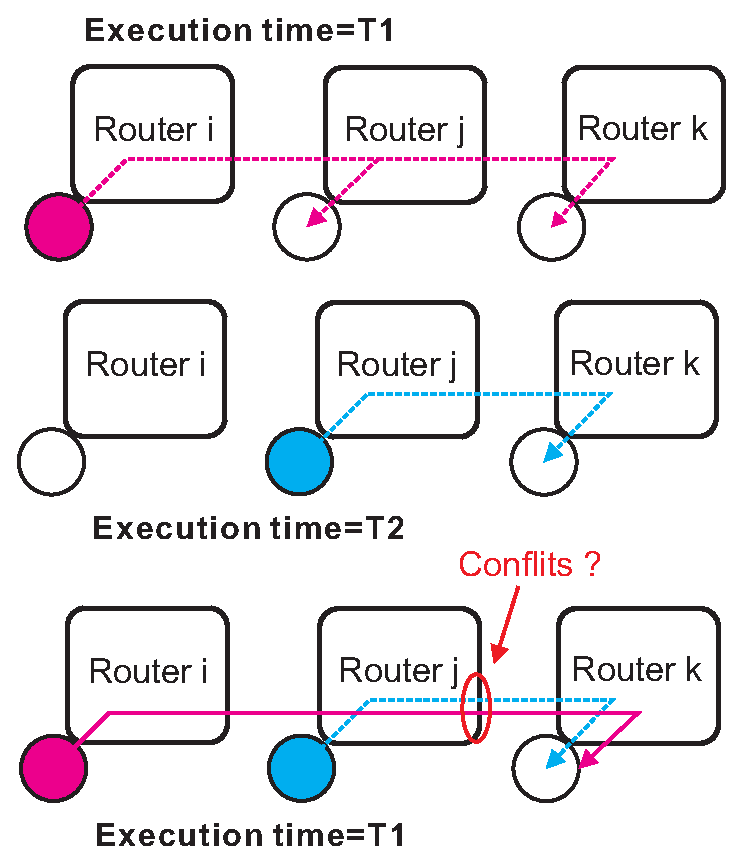
\includegraphics[width=0.6\columnwidth]{router.eps}
  \vskip -2mm
  \caption{An example of how a data dependency has an impact on traffic behaviors.}
  \label{fig:router}
  \vskip -8mm
\end{figure}
\subsubsection{Vision of the Model}
An application consists of different tasks and their interactions (i.e., inter-task data and non-data dependencies). To analyze the structure and dynamics of its tasks, one can represent the application using graphical models where tasks are represented as nodes and task interactions as edges. In spite of their wide use in validating the resource scheduling, task mapping, automatic parallelization as discussed in Section 2, their application to modeling the runtime application traffic behaviors is limited. For instance, communication task graphs (CTG) used in prior NoC studies are not able to capture dynamic data dependencies, i.e., when a data set is generated,  exchanged and how different data sets are related at runtime. Ignoring such dependencies might lead to biased network performance measurement. To give an intuition, we show a simple PE-based NoC example in which ignoring the data dependencies can lead to erroneous estimates of the NoC performance for an application of interest. \\
\indent Figure~\ref{fig:router} shows three routers $i, j$ and $k$ (each with a single input buffer) interfacing three processing elements (PEs) and exchanging data for calculating the average and variance of a time series stored in tile $i$. Let us assume PE $i$ sends this data to PEs $j$ and $k$. The results computed by PE $j$ will be reused by PE $k$, i.e., the average of the data set will be sent to PE $k$ for calculation of the variance, thus there is data dependency between these two tasks (i.e., calculation of average and variance). During execution, what really happens is that the packets issued by PE $j$ might never have conflicts with those injected by PE $i$ because the computation in PE $j$ usually takes more time than what it takes to move the data from PE $i$ to PE $k$. However, if we use a conventional CTG or even a trace-based benchmark that does not consider task dependencies, we might end up with erroneous network performance measurement. This happens when the link between Router $i$ and $j$ is heavily congested such that the packet injected by Router $i$ waits longer than the computation time of PE $j$. In such case, Router $j$ would still mistakenly inject the "results" as instructed by the collected trace even it has not received full data set from Router $i$, resulting in a unrealistic traffic pattern.\\
\indent To address these problems, we propose a dynamic graphical model learned at runtime not only for accurate characterization of the application but also practical use as realistic traffic generator. More precisely, we propose to model each task as a data generation system, which consists of: i) a timed finite state machine that governs its system state transition at runtime and ii) a data generation process that determines its communication patterns. By relating the input of the system to the system state transition that determines the output in a timed fashion, the proposed model is able to capture runtime inter-task dependencies and characterize the spatio-temporal patterns of the communication.
\subsubsection{Model Description}
%The keystone of the model is to set up an abstraction of \textit{task} to understand what it is and how it affects the communication. A intuitive description of a task given a specific application is a component that takes data from upstream tasks or user entries as input, performs an operation on those data, and generate a new set of data as output for tasks in the subsequent execution path and send them following a certain pattern, i.e., a specific distribution of data generation. Given a fixed task, a different set of data input might result in different set of output and the associated data generation process,  based on the state of task execution. Consequently, instead of modeling a task as a single node, we define the task as a data generation system with following formalism, \\
%so the system stata pathway matters ! 

The keystone of the model is to set up an abstraction of the application that is able to not only mathematically expressive in capturing the runtime application behaviors and its task structure, but also practically easy to be learned and used for realistic traffic generation. Towards this end, we follow the same idea to characterize a parallel program from a compiler perspective and define an application as a collection of tasks. Each task can be understood as a sequence of basic operations. Given a task, its execution might have i) data dependencies (i.e., it requires the output of other tasks) and/or ii) non-data dependencies (e.g., synchronization) on prior tasks. Once these dependencies are satisfied, the behaviors of tasks can be summarized as: i) processes its input (either from prior tasks or from user input), ii) generates a new set of data as output for tasks in the subsequent execution path and iii) exchanges them following a specific pattern (i.e., a specific distribution of data generation). Intuitively, a task can be abstracted as data generation system: it checks upon its input and transits its state from IDLE to READY as its dependencies on prior tasks are satisfied over time. If the system enters READY, it will operate on its input and map them to output over an execution time horizon. Otherwise, it will keep still and waiting for the receipt of all its input. To formally characterize it, we introduce the following definition:\\
\noindent \textbf{Definition 1:}\label{def:task} \textit{ An application task $\mathcal A(t)$ is a data generation system determined uniquely by a quadruple $(\mathcal M, \mathcal G(t), \mathcal T, \mathcal C)$  over time horizon $[t,t+\mathcal T]$. $\mathcal M$ is a timed finite state machine. \{$\mathcal G(t)$, $t\in \mathcal T$\} is a data generation process where $\mathcal G(t')$ denotes the number of data units generated over time interval [$t,t+t'$]. Function $\mathcal C$ maps a task $\mathcal A(t)$ to a set $\mathcal C(\mathcal A(t))$  containing all other prior tasks upon which the execution of $A(t)$ has dependencies. } \\
\indent An application task $\mathcal A(t)$ is defined over its execution horizon $\mathcal T$, i.e., its active time period. To run task $\mathcal A(t)$, all prior tasks in $\mathcal C(\mathcal A(t))$ have to be finished. To check upon whether such dependencies are met over time, $\mathcal A(t)$ maintains a timed state machine $\mathcal M$ to drive system state transition from IDLE to READY. Upon READY, the execution will be initiated to generate a new set of data that might be used for subsequent tasks. The data generation can be characterized by a process \{$\mathcal G(t)$, $t\in \mathcal T$\}. To detail the timed state machine $\mathcal M$, we formally introduce the following definition:\\
 \noindent \textbf{Definition 2:}\label{def:machine} \textit{ A timed finite state machine $\mathcal M$ is a sextuple $(\mathcal I,\mathcal S, s_{0}, \mathcal O,\mathcal F, \Omega$) where $\mathcal I,\mathcal S,$ and $\mathcal O $ are finite disjoint sets of inputs, states and outputs, respectively. $s_{0}$ is the initial state. $\mathcal F$ is the transition function $\mathcal F: 2^{\mathcal I} \times \mathcal S \times 2^{\mathcal T} \rightarrow \mathcal S$. $\Omega$ is the output function $\Omega: \mathcal S\times \mathcal T \rightarrow 2^{\mathcal O}\times 2^{\mathcal T}$.}\\
 \indent Of note, $\mathcal I$ and $\mathcal O$ are the input and output alphabet with finite symbols, respectively. The idea is to introduce these two sets to model the input and output of a task. $\mathcal I$ and $\mathcal O$ provide abstract description of different dependency types. In practice, we use a simple integer alphabet $\{0,1,2\}$ for both $\mathcal I$ and $\mathcal O$. The input is $"0"$ if no corresponding dependency is met. Otherwise, $"1"$ and $"2"$ denote data dependency or non-data dependency, i.e., synchronization requirement, is satisfied, respectively. We use the finite alphabet set to avoid any architecture-specific assumptions, e.g., type of data or width of channels, such that the model is self-contained and general without a specific machine model, which might limit the applicability of the formalism.\\
  \indent $\mathcal F$ is a \textit {timed} transition function that maps a vector of inputs $I(\mathcal A(t))=\{i_k|i_k \in \mathcal I\}$, the current state $s \in \mathcal S$ and a vector of time stamps \{$t_k$\} associated with $I(\mathcal A(t))$ to the next state.  We refer to $i_k \in I(\mathcal A(t))$ as an input channel and $|I|$ is the width of input channel. Each input channel  $i_k \in I(\mathcal A(t))$ is paired with a time stamp $t_k$ (denoted as $(i_k, t_k)$) which determines the earliest time that $i_k$ can be checked. We introduce this time stamp to consider the time cost of task execution and communication which will be later detailed in the discussion of output function $\Omega$. Each $i_k$ connects to an output of an upstream task on which the execution of task $\mathcal A(t)$ depends, thus $|I(\mathcal A(t))|=|\mathcal C(\mathcal A_{t})|$. The task dependency of $\mathcal A(t)$ on a prior task $\mathcal A'(t)$ is satisfied if and only if a letter $"1"$ or $"2"$ in $\mathcal I$ is received by input channel $i_k \in I(\mathcal A(t))$ and its associated time stamp $t_k$ is not greater than current time stamp $t$ when the transition condition is being checked, i.e., the causal constraint. In contrast to ordinary finite state machine, we introduce an extra \textit{temporal} dimension to guard the state transition such that the timing information of the application can be captured. Consequently, the transition function $\mathcal F$ would drive the system state into READY if and only if $i_k \neq 0$ and $t_k \leq t$, $\forall i_k  \in I(\mathcal A(t))$.\\
  \indent The output function $\Omega$ maps the timed current state $(s,t)$, where $s\in\mathcal S$ and $t \in \mathcal T$,  to a vector of output $O(\mathcal A(t))=\{o_k|o_k \in \mathcal O\}$, guarded by an array of time stamps \{$t+\delta_k$\}. Similarly, we define $o_k \in O(\mathcal A(t))$ as an output channel.  $\delta_k$ denotes the \textit{delay} of output channel $o_k$ caused by the execution of the task on the input data set $I(\mathcal A(t))$ and the data generation process, i.e., communicate data over a certain period of time, is equal to $\delta_{k,e}+\delta_{k,c}$, the execution delay and communication delay, respectively. Of note, $\delta_{k,e}$ replies on mapping function from the task to a specific processing entity (e.g., a dedicated PE or a processor), i.e., the delay is decided by how "fast" the task can be processed. In the model, we have no assumption on mapping function or processing entity, hence enhancing the expressivity of the model. $\delta_{k,c}$ is the \textit{span} of the data generation process which is described by $\mathcal \{\mathcal G(t), t\in \mathcal T\}$. Given a specific task, the data generation process could be arbitrarily complicated whereas it is still possible to find a \textit{best-fit} stochastic process model that best characterize its behaviors. For instance, the process could be memory-less (e.g., Poisson process), long-range memory (e.g., self-similar or fractal process) or a general $\alpha$-stable process.\\
  \indent Connecting Definition~1 and 2, we have constructed the backbone of the model for NoC applications. Compared to the conventional definition of task in context of parallel program analysis, we view each task as a data generation process whose behaviors are governed by a timed state machine $\mathcal M$ and data generation process $\mathcal G(t)$ given the execution time horizon $\mathcal T$. Its dependencies are characterized by $\mathcal C(\mathcal A(t))$.  Given a collection of tasks $A=\{\mathcal A_i(t)\}$, we are able to construct a graphical model $\mathcal B(t)=(A,E,t)$ where each vertex $a_i$ corresponds to an application task $\mathcal A_i(t)$ and each directed edge $e_{i,j}$ exists if and only if task $a_i$ has, either data or non-data, dependency on task $a_j$. Formally, we have the following definition,\\
\noindent \textbf{Definition 3:}\label{def:app} \textit{ A NoC application $\mathcal B(t)=(A,E,t;\mathcal T)$ over its execution time horizon [$t$,$t+\mathcal T$] is a \textbf{dynamical directed graph} where each vertex $a_{i} \in A$ is an application task $\mathcal A_i(t)$ and edge $e_{i,j} \in E$ if and only if $\mathcal A_{j}(t) \in \mathcal C(\mathcal A_{i}(t))$.}\\
\indent In contrast to previous graphical model for application traffic, the proposed model not only translates the spatial dependencies into geometric characteristics of the graph (i.e., nodes, edges and their connection pattern), but also introduces a detailed description for tasks that are able to preserve the temporal dependencies. In the following discussion, we will present a traffic synthesis technique based on the proposed model to address the problem \textbf{P$_2$)}.
\subsection{Benchmark Workloads synthesis}
The large-scale benchmark synthesis problem can be stated as follows: \textit{How can the traffic be generated for a given size and the application profiled by the proposed model $\mathcal B(t)=(A,E,t;\mathcal T)$ such that traffic characteristics of the real application are preserved ?}. Thus, our objective is to build a traffic generator for NoC evaluation without interfacing it with a full-system simulator such that, the target NoC is identically stressed but requires less simulation time. \\
\indent To formally define the problem, let $A$ be the universal set of tasks involved in $\mathcal B(t)$. Assume $|A|=n$, let $S(t)$ be the $n$-dimensional state vector of $\mathcal B(t)$ such that $S(t)=[s_0(t),s_1(t),\dots,s_{n-1}(t)]^{T}$. We define the vector sequence $E_0=$<$S(0),S(\Delta t),S(2\Delta t),...$ $S(\mathcal T)$> as the \textit{recorded states of tasks during application execution on target architecture over finite horizon $[0,\mathcal T]$}. In other words, $E_{0}$ is the task state transition trace recorded from the execution of the real application. We define $E(\mathcal B(t))$ = < $S(0)$, $S(\Delta t)$, $S(2\Delta t)$$,...,$ $S(\mathcal T)$> as \textit{an execution of benchmark $\mathcal B(t)$ over a finite horizon $[0,\mathcal T]$} where $\Delta t$ is time step of interested length, i.e., the cycle of simulation clock. Intuitively, $E(\mathcal B(t))$ is the simulated system state transition trace. Since it is observed that the output of each task is \textit{uniquely} decided by the system state $s$ and the time stamp $t$ through the mapping relation $\Omega$ for each task $\mathcal A_{i}(t)$ (see Definition 2). Therefore, the system state transition trace determines the traffic characteristics of the application. As a result, given an execution horizon $\mathcal T$, ideally, the simulated system state transition trace  $E(\mathcal B(t)) $ should be equal to the recorded state trace $E_0$. Formally, we can formulate the benchmark synthesis problem  as :\\\\
\noindent\textbf{NoC benchmark synthesis problem :} \\
\textbf{Given} an application profiled by $\mathcal B(t)$, a target architecture, execution time $\mathcal T$ and the recorded application state transition trace $E_{0}$ \\
\textbf{Determine} the initial state $s_0$, output function $\Omega$ and data generation process $\mathcal G(t)$ for each task $\mathcal A_{i}(t)$ to obtain an execution $E(\mathcal B(t))$ of $\mathcal B(t)$ to minimize its deviation from the recorded trace: 
\begin{equation}\label{eq:prb1}
   \min\limits_{s_0,\Omega,\mathcal G(t)} ||E(\mathcal B(t))-E_0||^2
\end{equation}
Equation~\ref{eq:prb1} shows the proposed model enables us to provide a way to quantify the similarity of the characteristics between the synthesized traffic and the real application traffic by measuring the norm of deviation of state transition trace in both cases. \\
\indent To solve this problem, it should be first noted that the source of difficulty in minimizing~(\ref{eq:prb1}) resides  both in accurately identifying the task structures, i.e., tasks and their runtime inter-dependencies, and capturing its communication patterns (e.g.,g memory access events), i.e., learning the data generation process $\mathcal G(t)$. We thus propose a synthesis framework based on runtime architecture-independent model learning. Figure \ref{fig:OVERVIEW} shows the overview of the proposed benchmark synthesis framework. The overall framework could be understood as a two-stage process where i) an \textit{architecture-independent} application profiling and model learning stage is set up for analysis of runtime application task graph and construction of the NoC application model $\mathcal B(t)$ upon which ii) a subsequent benchmark generating stage is built to introduce realistic variation to the generated traffic model for extrapolated traffic synthesis given a \textit{target} architecture. It should be noted that, instead of extracting static task graphs, we define NoC application model $\mathcal B(t)$ in Section 3.2.2 as a dynamical graph that can only be learned during the execution of the program. This is because the statically extracted task graph is not a sufficient representative of the applications with unknown tasks and their spatio-temporal inter-task dependencies prior to execution of them.\\
\indent Specifically, we have modified the Contech compiler~\cite{railing2015contech} that is based on the LLVM compiler framework~\cite{lattner2004llvm} with OpenMP support that provides the ability to observe and manipulate the intermediate representation of a program. Following Contech compiler, the adopted profiling methodology is two-layered. The first layer is used to take the source code of the application as input and translate it into instrumented LLVM intermediate representation(IR).  The compiler in the \textbf{first layer} will run a function-by-function check to identify the basic blocks (e.g., basic actions or predefine functions) and insert inlined codes into target ISA assembly to collect the properties of memory access events, i.e., address, size, type and timing information \textit{during the execution time of the application}. To capture the inter-task dependencies, the synchronizing actions are identified through analyzing the LLVM IR or the name of the function invoked. The address of the action, the order of the action with respect to other synchronization actions on this address and time stamps from before/after the action will be recorded in a local buffer for each thread. Eventually, a global event list will be generated where events from the same thread are stored in the \textit{event list in program order} rather than the micro-architectural order from out-of-order processors or memory consistency, thus avoiding specific architectural assumptions. \\
\indent \textbf{The second layer} takes the extracted event list to infer the application model $\mathcal B(t)$. Each task accumulates a list of basic block IDs and memory accesses from the event list until a synchronizing action is encountered. Then all previous blocks are assumed to be in the same \textit{context} and merged into a single task $\mathcal A_{i}$. The task dependencies between other synchronizing actions are checked such that for each $A_{i} \in \mathcal B(t)$, we are able to determine the input channel $\mathcal I(\mathcal A_{i})$ (or output channel, equivalently) upon finishing processing all basic blocks in the event list. Alternatively stated, we are capable of construction of node $\mathcal A_{i}$ and edge $e_{i,j}$ of all choice of $i$ and $j$ for $\mathcal B(t)$ given the event list collected by the LLVM compiler with instrumentation at execution time. This constitutes the topology, i.e., the structural features, of the proposed graphical model. Recall that we define application task $A_{i}$ as a quadruple \{$\mathcal M,\mathcal G(t),\mathcal T, \mathcal C$\} where function $\mathcal C(A_{i})$ denotes the subset of tasks dependent on $\mathcal A_{i}$. By identifying tasks and their dependencies, we have learned also the function $\mathcal C$.\\
\indent To practically use the graphical model to generate traffic aligned with realistic application behaviors, we should derive finite state machine $\mathcal M$ and data generation process $\mathcal G(t)$ also from the collected trace in the first layer. We define each input channel of a task to correspond to the dependency on a upstream task. The state transits as any of its dependencies on prior tasks are met, i.e., either data or synchronizing dependencies are satisfied. The date generation process $\mathcal G(t)$ is initiated once the state machine $\mathcal M$ enters the end state where all dependencies are satisfied. Recall that we have recorded all memory access events by running the instrumented program. All memory access events, when mapped to a NoC-based architecture, translate to data injection events. Combined with time stamp of the memory accesses recorded, it is possible to either i) directly use the trace or ii) fit a stochastic process $\mathcal G(t)$ for data injection of each task $\mathcal A_{i}$. Together with execution horizon $\mathcal T$ which we use to run the program, we have learned the application traffic model $\mathcal B(t)$.\\
 \indent It should be noted that fitting a stochastic process $\mathcal G(t)$ to the recorded data generation process could be arbitrarily difficult as it might not be aligned with a known stochastic process or changes quickly over time such that we do not have sufficient data for estimation of the distribution parameters. Otherwise, we can fit a stochastic model to \{$\mathcal G(t),t$\} to further reduce the complexity of the model. As a case study, we assume $\mathcal G(t)$ follows a Poisson distribution such that for output channel $o_k$: 
\begin{equation}\label{eq:poisson2}
   P\{\mathcal G(\Delta t)=k\}=\frac{\lambda \Delta t^{k}}{k!}e^{-\lambda \Delta t}
\end{equation}
$\lambda$ is the strength of Poisson flow. Given the size of data to be generated as $L$, the statistical average of $\delta_{k,c}$ is given by,
\begin{equation}\label{eq:solu}
   \textbf{E}[\delta_{k,c}]=\frac{L}{\textbf{E}[\mathcal G(\Delta t)]}\Delta t 
\end{equation}
Since $\textbf{E}[\delta_{k,c}]$ is an unbiased estimate of $\delta_{k,c}$, we use $\textbf{E}[\delta_{k,c}]$ to replace $\delta_{k,c}$. Of note, the assumption of Poisson distribution is helpful to give a case study whereas Equation~(\ref{eq:solu}) can be applied to other processes.\\
\indent Given the constructed model $\mathcal B(t)$, a follow-up question is how can we make changes to the graphical model such that i) we can simulate the runtime variations of the traffic (i.e., Problem \textbf{P}$_3$), and ii) how can we scale it to test different NoCs while preserving its spatial-temporal characteristics of traffic (i.e., Problem \textbf{P}$_2$). Next, we address these problems by proposing a network generation algorithm based on complex network theory. 
\section{Evolvable Benchmark Synthesis}
\subsection{Overview}
Given an application described by the proposed model $\mathcal B(t)$, it is desirable to generate an array of benchmarks that are diverse in scales but ``similar" in spatial and temporal behaviors as the $\mathcal B(t)$. As we discussed in Section 3, the spatial dependencies are encoded by the structural characteristics of $\mathcal B(t)$ while the temporal dependencies are embedded in structure of the task (i.e., the timed finite state machine $\mathcal M$ and the data generation process $\mathcal G(t)$).  Therefore, an efficient way to preserve such dependencies when editing the graph is to keep \textit{key structural features} of the model at \textit{proper scales}. For example, if we look at the graphical model at the highest scale, we will observe a single node. Then we replicate this single node and go back to the original scale. We will expect a very similar graph as the original one but doubled in size. Following the same idea, we can preserve any structure in the graph as long as we replicate a coarsened node at a proper scale. More precisely, we propose a scaling algorithm based on complex network generation that produces graphs that are similar to $\mathcal B(t)$. 
\subsection{Measuring the Graph Similarity}
\begin{figure}%[htb]
  \centering
  % Requires \usepackage{graphicx}
 % \epsfig{file=t_calc.eps}
  \includegraphics[width=1\columnwidth]{assort.eps}
  \vskip -2mm
  \caption{Example graphs visualize assortativity, betweenness and clustering }
  \label{fig:assort}
  \vskip -3mm
\end{figure}
\begin{figure}[t]
  \centering
  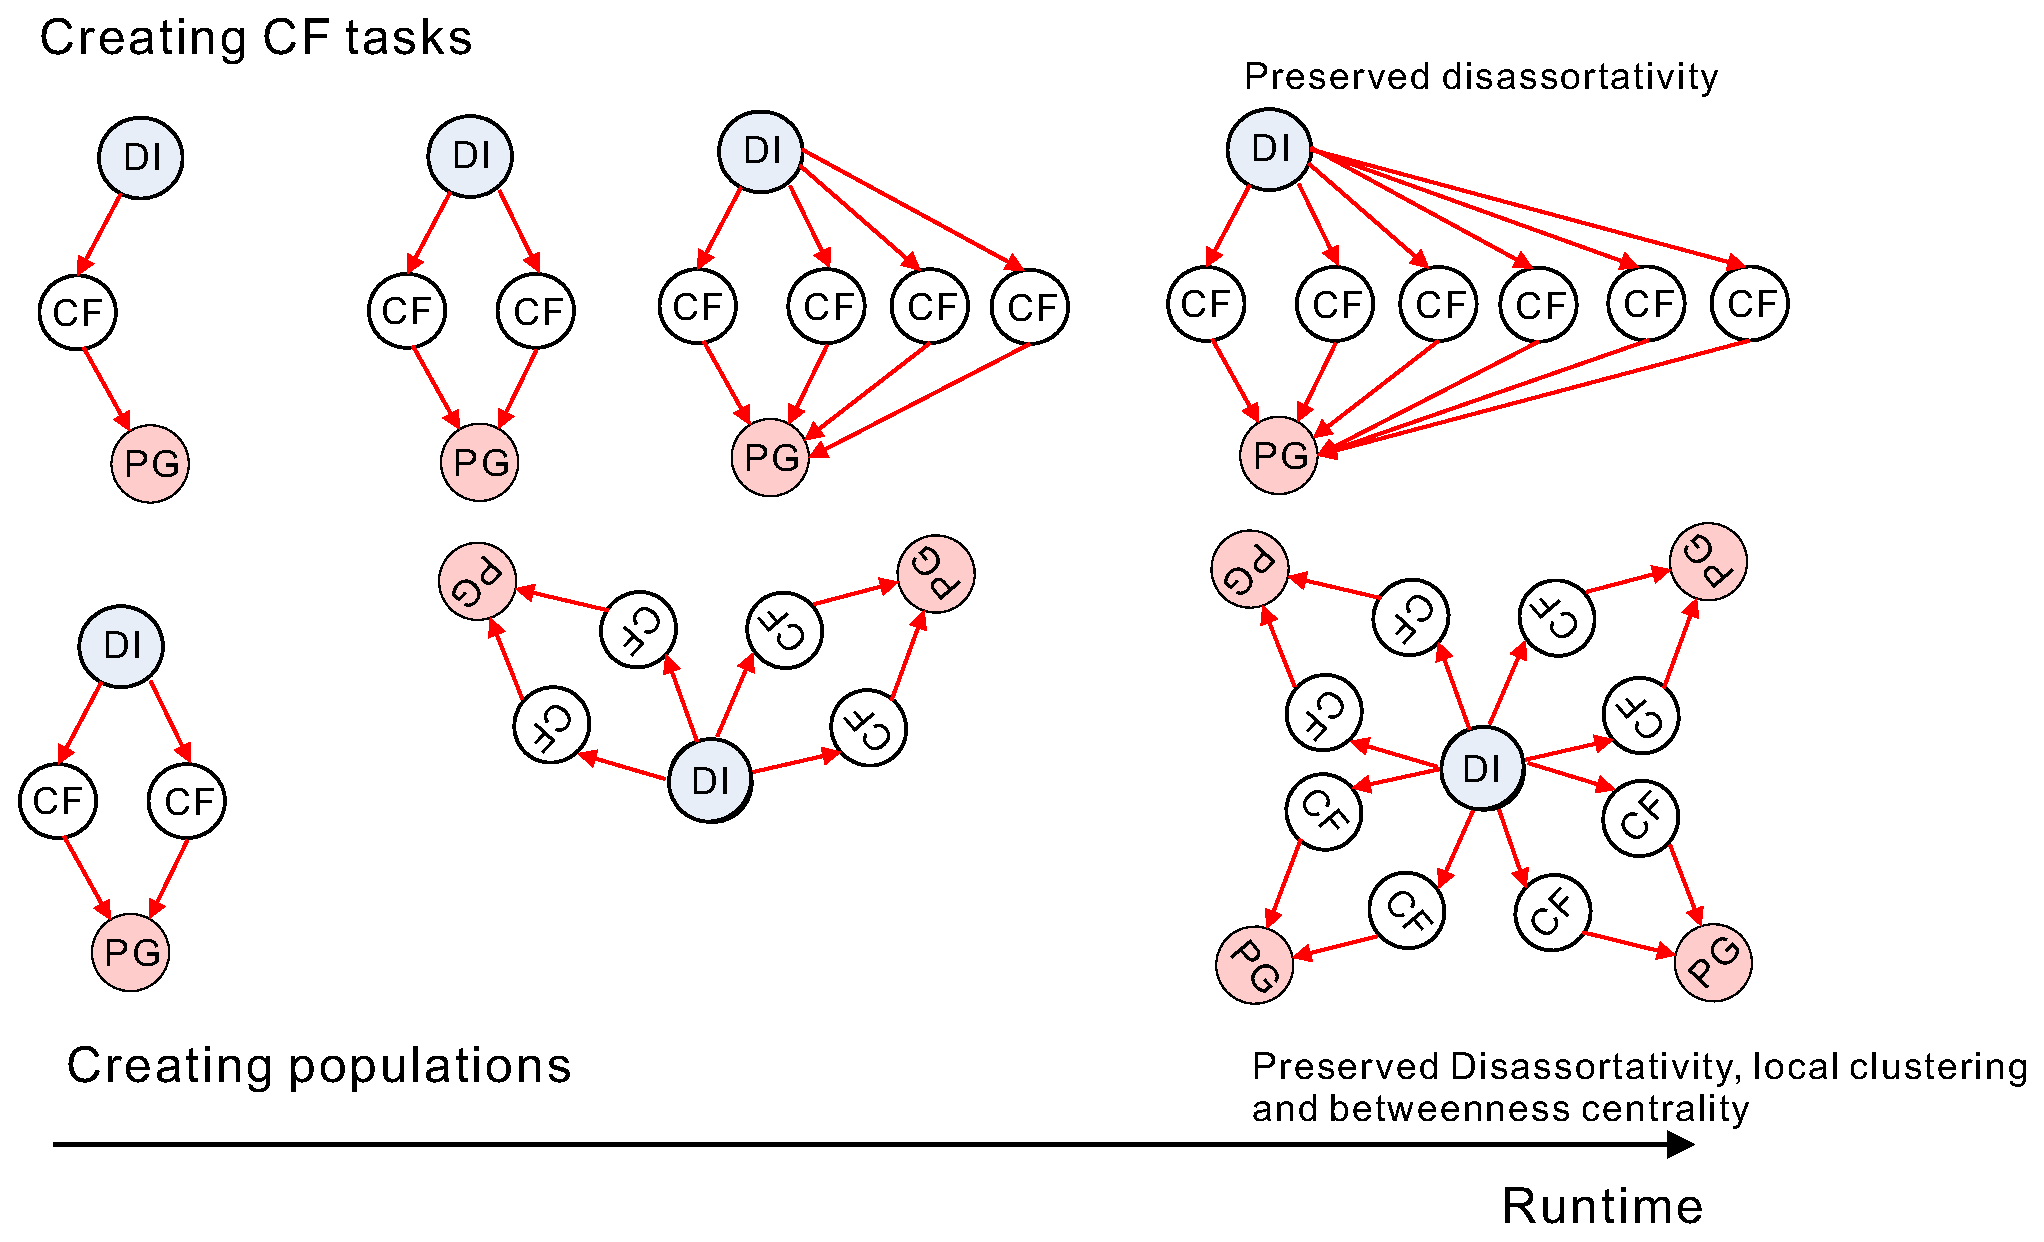
\includegraphics[width=1\columnwidth]{evl.eps}
  \vskip -2mm
  \caption{The evolution of genetic algorithm at runtime.}
  \label{fig:fig_evl}
  \vskip -5mm
\end{figure}
To measure the similarity between graphs of various sizes, we introduce a set of structural metrics $M=\{\alpha, \beta, \gamma, D_{avg}, P_{avg}\}$ which are well used for comparing graphs. The average node degree $D_{avg}$ shows the local interconnection strength. The average path distance $P_{avg}$ shows the average distance between all possible pairs of nodes in the graph.\\
\indent We denote $\alpha$ as the \textbf{assortativity} metric which measures the tendencies of nodes to connect with other nodes that have similar degrees as shown in Figure~\ref{fig:assort}. For directed graphs, the \textit{in} and \textit{out}-assortativity are measured, respectively. In general, $\alpha$ lies between $-ˆ’1$ and $1$. When $\alpha = 1$, the network is said to have perfect assortative mixing patterns, when $\alpha$ = 0 the network is non-assortative, while at $\alpha = -ˆ’1$ the network is completely disassortative. The \textbf{clustering coefficient} $\gamma$ is a measure of the degree to which nodes in a graph tend to cluster together. The \textbf{betweenness centrality} $\beta$ is an indicator of a node's centrality in a network. It is equal to the number of shortest paths from all vertices to all others that pass through that node. Betweenness has important implications for the proposed graphical model. To give an intuition, we visualize these metrics in Figure~\ref{fig:assort} using example graphs.\\
\indent To understand the physical meaning of the metrics and motivate their link to the task structures in a realistic setting, we present a case study where we run the multi-threaded coarse grain hierarchical parallel genetic algorithm (HPGA)  and show variations in task structure over time in Figure \ref{fig:fig_evl}. The sequential version of HPGA has very simple  task structure consisting of three basic blocks: i) Distribution of individuals (DI), i.e., candidate solutions; ii) Calculation of fitness (CF); iii) Produce the new generation (PG) based on fitness. In the example, the host is able to create new CF tasks and populations, i.e., a pool of candidate solutions, to parallelize the execution. Over the execution time, the task structure has been through variations whereas preserving several important structural features: i) The disassortativity of the graph is respected and preserved, i.e., nodes of high degree tend to connect to nodes with low degree. The task graph of HPGA is strongly disassortative suggesting the existence of global synchronization nodes. ii) The majority of nodes remains less clustered which indicate the source of potential parallelism; iii) The DI task preserves its high betweenness centrality as multiple populations and corresponding CF and PG tasks being created, which suggests DI as a synchronization node.\\
\indent  Even though the example is just a case study with very simple task structure, yet we can make the following observations: i) The structural feature analysis on the extracted application task graph can help us identify the critical tasks such as synchronization node and potential parallelism. ii) By preserving key structural features like assortativity (not necessarily the absolute value of the metrics), we might be able to introduce realistic variations to the original task graph especially when we have no prior knowledge on how the real application changes over time. Based on these observation, we next present our benchmark scaling algorithm.
\subsection{A Complex Network-inspired Benchmark Scaling}
\begin{algorithm}[tb]         %Ëã·¨µÄ¿ªÊ¼
\caption{Benchmark scaling algorithm  \textbf{Gen}($\mathcal B(t)$)}             %Ëã·¨µÄ±êÌâ
\label{alg:main}                  %¸øËã·¨Ò»¸ö±êÇ©£¬ÕâÑù·½±ãÔÚÎÄÖжÔËã·¨µÄÒýÓÃ
\begin{algorithmic}[1]                %²»Öª[1]ÊǸÉÂïµÄ£¿
\REQUIRE ~~\\

    Graph seed $\mathcal B(t)$; Selected metric set $M'\in M$; 
    Downscaling function $\Gamma$; Upscaling function $\Gamma^{-1}$; Editing function $\Pi$; Expected size of graph $N$                

\ENSURE ~~\\                           %Ëã·¨µÄÊä³ö£ºOutput
    A set of accepted graphs  \textbf{$\mathcal B'(t)$}
\STATE i=0;
\IF{Sanity\_check$(\mathcal B(t))$==false}
\STATE Return $\mathcal B(t)$
\ELSE
\STATE $\mathcal B'(t)$=$\Gamma(\mathcal B(t))$
\STATE $\mathcal B'(t)$=\textbf{Gen}($\mathcal B'(t)$)
\WHILE{$ |V'(t)|<N $ and $||M'(\mathcal B(t))-M'(\mathcal B'(t))||_{2} > \Delta$}
\STATE $\mathcal B(t)_{scaled}$=$\Gamma^{-1}(\mathcal B'(t))$
\STATE $\mathcal B'(t)$=$\Pi(\mathcal B(t)_{scaled})$
\ENDWHILE
\STATE Return $\mathcal B'(t)$
\ENDIF
\end{algorithmic}
\end{algorithm}
Let us define the editing function as $\mathcal E: V\times E \rightarrow V\times  E$ and $M(\mathcal B(t))$ as the similarity vector under above-mentioned metrics $M$. The problem to generate evolvable benchmarks can be formally stated as:\\\\
\noindent\textbf{NoC benchmark scaling problem} \\
 \textbf{Given} an application profiled by $\mathcal B(t)$ and the metrics of interest $M'\subset M$.\\
 \textbf{Determine} a sequence of editing function $\mathcal E=$ <$\mathcal E_0,...,\mathcal E_{n-1}$> such that
\begin{equation}\label{eq:prb_evl}
 \min\limits_{\mathcal E_0,...,\mathcal E_{n-1}} ||M'(\mathcal B(t))-M'(\mathcal E(\mathcal B(t)))||^2
\end{equation}
\textbf{Subject to:} 
\begin{equation}\label{eq:prb_SUB}
|V'(t)|\geq N, V'(t) \in \mathcal E(\mathcal B(t))
\end{equation}
Starting with a $\mathcal B(t)$ as seed, we need to determine a series of editing functions applied to $\mathcal B(t)$ to generate $\mathcal B'(t)$ such that a subset of structural features $M'$ are preserved. \\
\noindent \textbf{Lemma 1:}\label{def:causal}
\textit{The problem described by~\eqref{eq:prb_evl} is NP-hard}.\\
\textit{Proof:} The proof follows by noticing that the calculation of the average path of a graph requires finding all the paths in a graph. Thus the problem solution contains the solution to  the longest path problem, which is NP-hard. Because the problem in~\eqref{eq:prb_evl} contains (as subclass of problems) one that is NP-hard, it follows that \eqref{eq:prb_evl} is also NP-hard.\\
\begin{figure}%[htb]
  \centering
  % Requires \usepackage{graphicx}
 % \epsfig{file=t_calc.eps}
  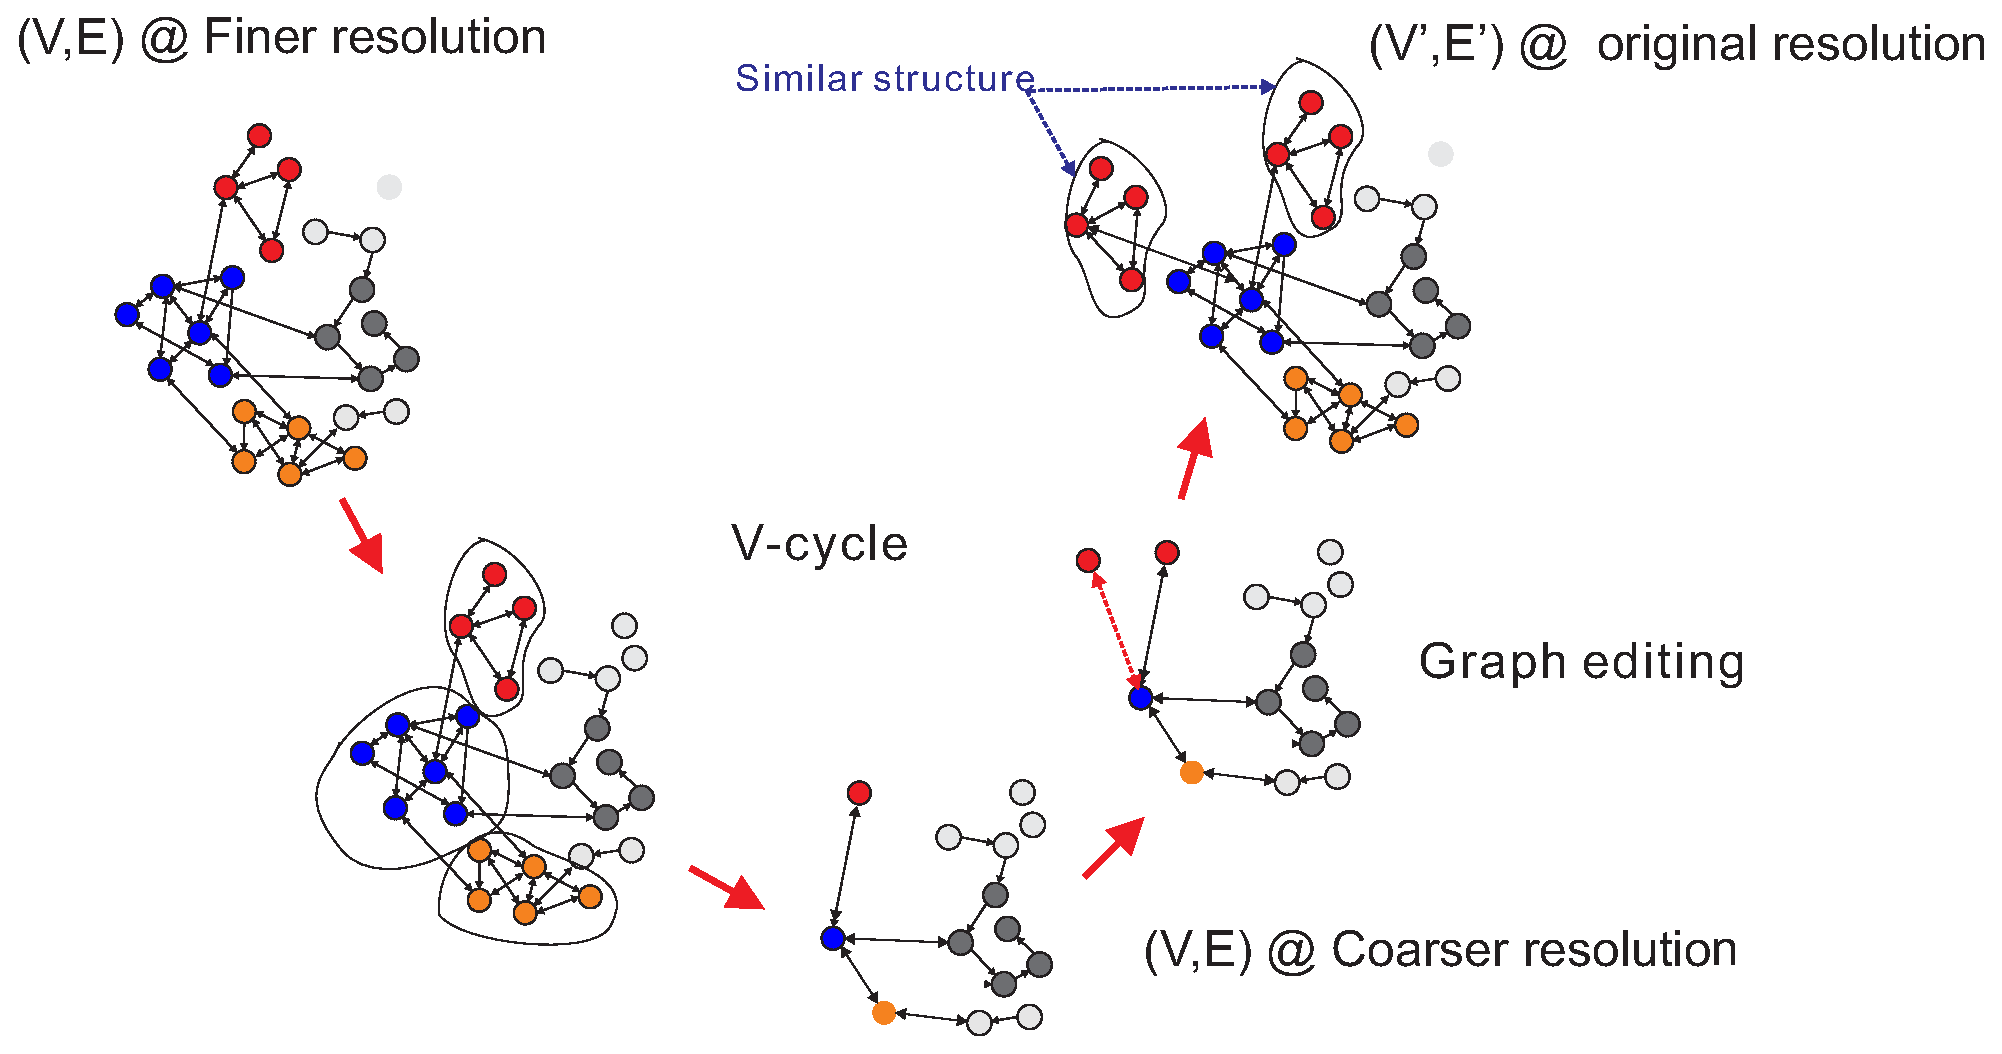
\includegraphics[width=1\columnwidth]{V.eps}
  \caption{The overview of benchmark scaling algorithm. The procedure follows a V-cycle of coarsening and refining operations. By preserving nodes under proper scales, it is able to protect the  structural features of interest.}
  \label{fig:V}
  \vskip -5mm
\end{figure}
\indent Therefore, we propose a heuristic to solve this problem, which is inspired by the complex network generation and multiscale theory applied to solve combinatorial optimization problem in \cite{ron2011relaxation}. Alg. \ref{alg:main} shows the overall procedure of proposed algorithm. The proposed algorithm is a V-cycle scheme that solves the problem described in~\eqref{eq:prb_evl} using coarsening and refining iterations at multiple scales as shown in Figure~\ref{fig:V}. Our proposed algorithm starts from a seed application profiled by graph $\mathcal B(t)$ and recursively change the graph into greater scales (i.e. upscaling) until a sanity check is violated. The sanity check will control how deep the V-cycle would go by setting a lower bound for both number of nodes and edges remained. Once violated, the upscaling stops. Then an array of downscaling functions are applied to project the graph with ``coarser details" to a graph of a finer resolution. After the graph is downscaled,  a series of editing functions, i.e., node replication, insertion or deletion, are performed. To scale the benchmark while preserving the structural characteristics of the original graph, only node replication is considered. In other cases like simulation of application variation, there is no restriction on editing operations. 
\section{Experimental Results}

\noindent\textbf{Experimental setup}: To validate our mathematical framework for benchmark generation and scaling that preserve structural features of the extracted task graph, we consider three graph-based application traffic benchmarks, \textit{blackscholes, canneal and freqmine} from Parsec $2.1$.  We present two sets of experiments to validate the proposed application traffic model and NoC benchmark synthesis algorithms. \\
\indent In the first set of experiments, we compare i) the packet injection patterns and ii) average latency of the network during the execution of the region of interest (ROI), i.e., parallel phase, from a full-system simulation,  and those on a dedicated cycle-accurate NoC simulator driven by the traffic generated by the proposed model. We learn the model $\mathcal B(i)$ by instrumenting the applications and collecting execution trace. The full-system simulation is performed by Gem5 simulator  on 32- and 64-core in-order 2 GHz Alpha ISA processor running over a Linux kernel of version 2.6.27 which is patched for supporting 4-64 Alpha cores. The NoC interfaced with the processors is following the Garnet network model with mesh topology under deterministic dimension-order routing (DOR). The flit size is set as 8 bytes. Each input port has 4 virtual channels and the depth of each virtual channel is 4-flit. The dedicated NoC simulator is a cycle-accurate simulator written in C++ with settings that are identical to those used in full-system simulation.\\
\begin{figure}%[htb]
  \centering
  % Requires \usepackage{graphicx}
 % \epsfig{file=t_calc.eps}
  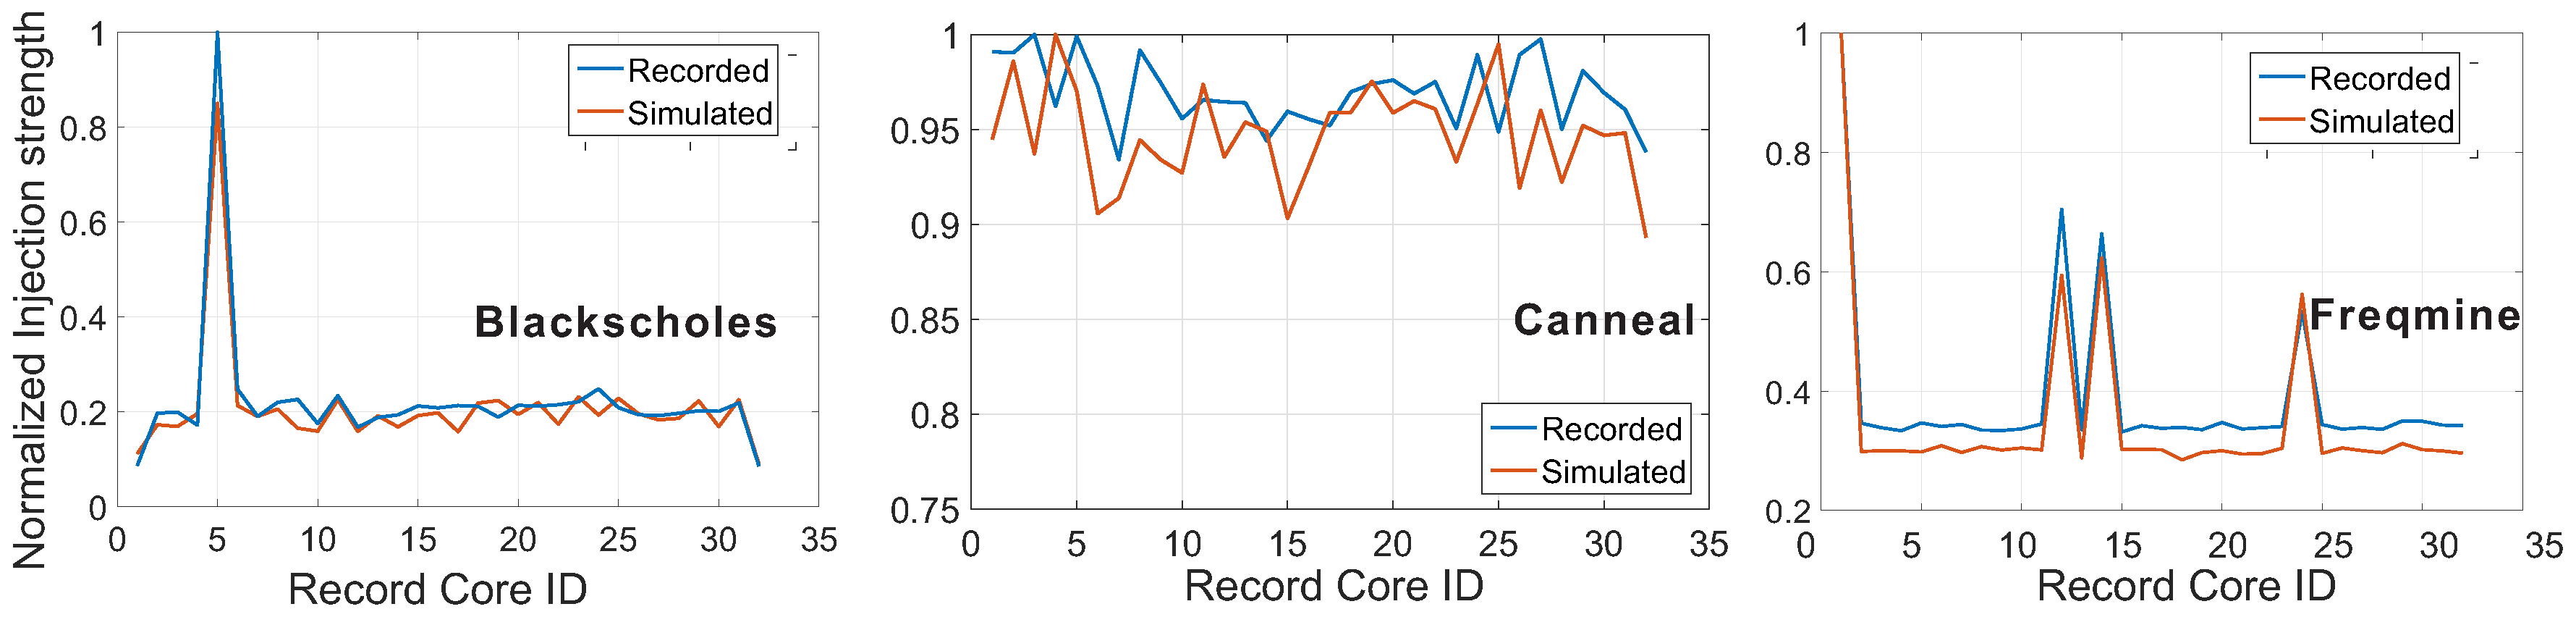
\includegraphics[width=1\columnwidth]{norm.eps}
  \vskip -2mm
  \caption{Measuring the distribution of injection strength over different processors under three application benchmarks, \textit{blackscholes, canneal and freqmine}, using both full-system simulation and synthesized traffic workloads based on the proposed model during ROI. The injection strength is calculated as the injection rate of a processor averaged over the execution time. In all three cases, the synthetic traffic workloads stress the target NoC to exhibit close injection distributions.}
  \label{fig:traffic_sim}
  \vskip -5mm
\end{figure}
\begin{figure}[ht]
  \centering
  % Requires \usepackage{graphicx}
 % \epsfig{file=t_calc.eps}
  \includegraphics[width=0.8\columnwidth]{latency.pdf}
  \vskip -3mm
  \caption{Comparison of average latency}
  \label{fig:lat}
  \vskip -5mm
\end{figure}
We first report three experiments performed under the full-system simulations using Gem5 on a 32-core system and the NoC stress test using a cycle-accurate C++ NoC simulator. To measure the goodness-of-fit of traffic behaviors using the synthetic traffic against those under the full-system simulation, i.e., whether the network communication exhibits close patterns under two workloads, we choose to measure the distribution of average injection strength during ROI over all 32 cores considered.  The average injection strength is calculated by averaging the total number of packets generated by the lapsed time. The results are reported in Figure~\ref{fig:traffic_sim} and normalized by the maximum injection strength of both cases. It is observed that the obtained distributions of injection strength under the synthesized NoC traffic are consistent with those measured during the full-system simulation in all three benchmarks. It should be noted that the injection strength distribution is contributed by all runtime communication and computation events that are either producing or consuming data. These events are inter-coupled via the task dependencies embedded in the execution path of the application.  Without the incorporation of such dependencies in the synthesized traffic, it is difficult to have close fitting to the real traffic behaviors that are usually identified through full-system simulation. In addition to injection strength distribution, we have also measured the average network latency for networks of different size driven by the full-system simulation trace or the generated traffic by the proposed model. The results are reported in Figure~\ref{fig:lat}. Under different network settings, the NoC simulation driven by the proposed model demonstrates consistently  close latency performance compared to that measured under full-system simulation with an error mean of $\%1.2$ and $\%2.1$ for 32-core and 64-core simulation, respectively.\\
\begin{figure}[tb]
  \centering
  % Requires \usepackage{graphicx}
 % \epsfig{file=t_calc.eps}
  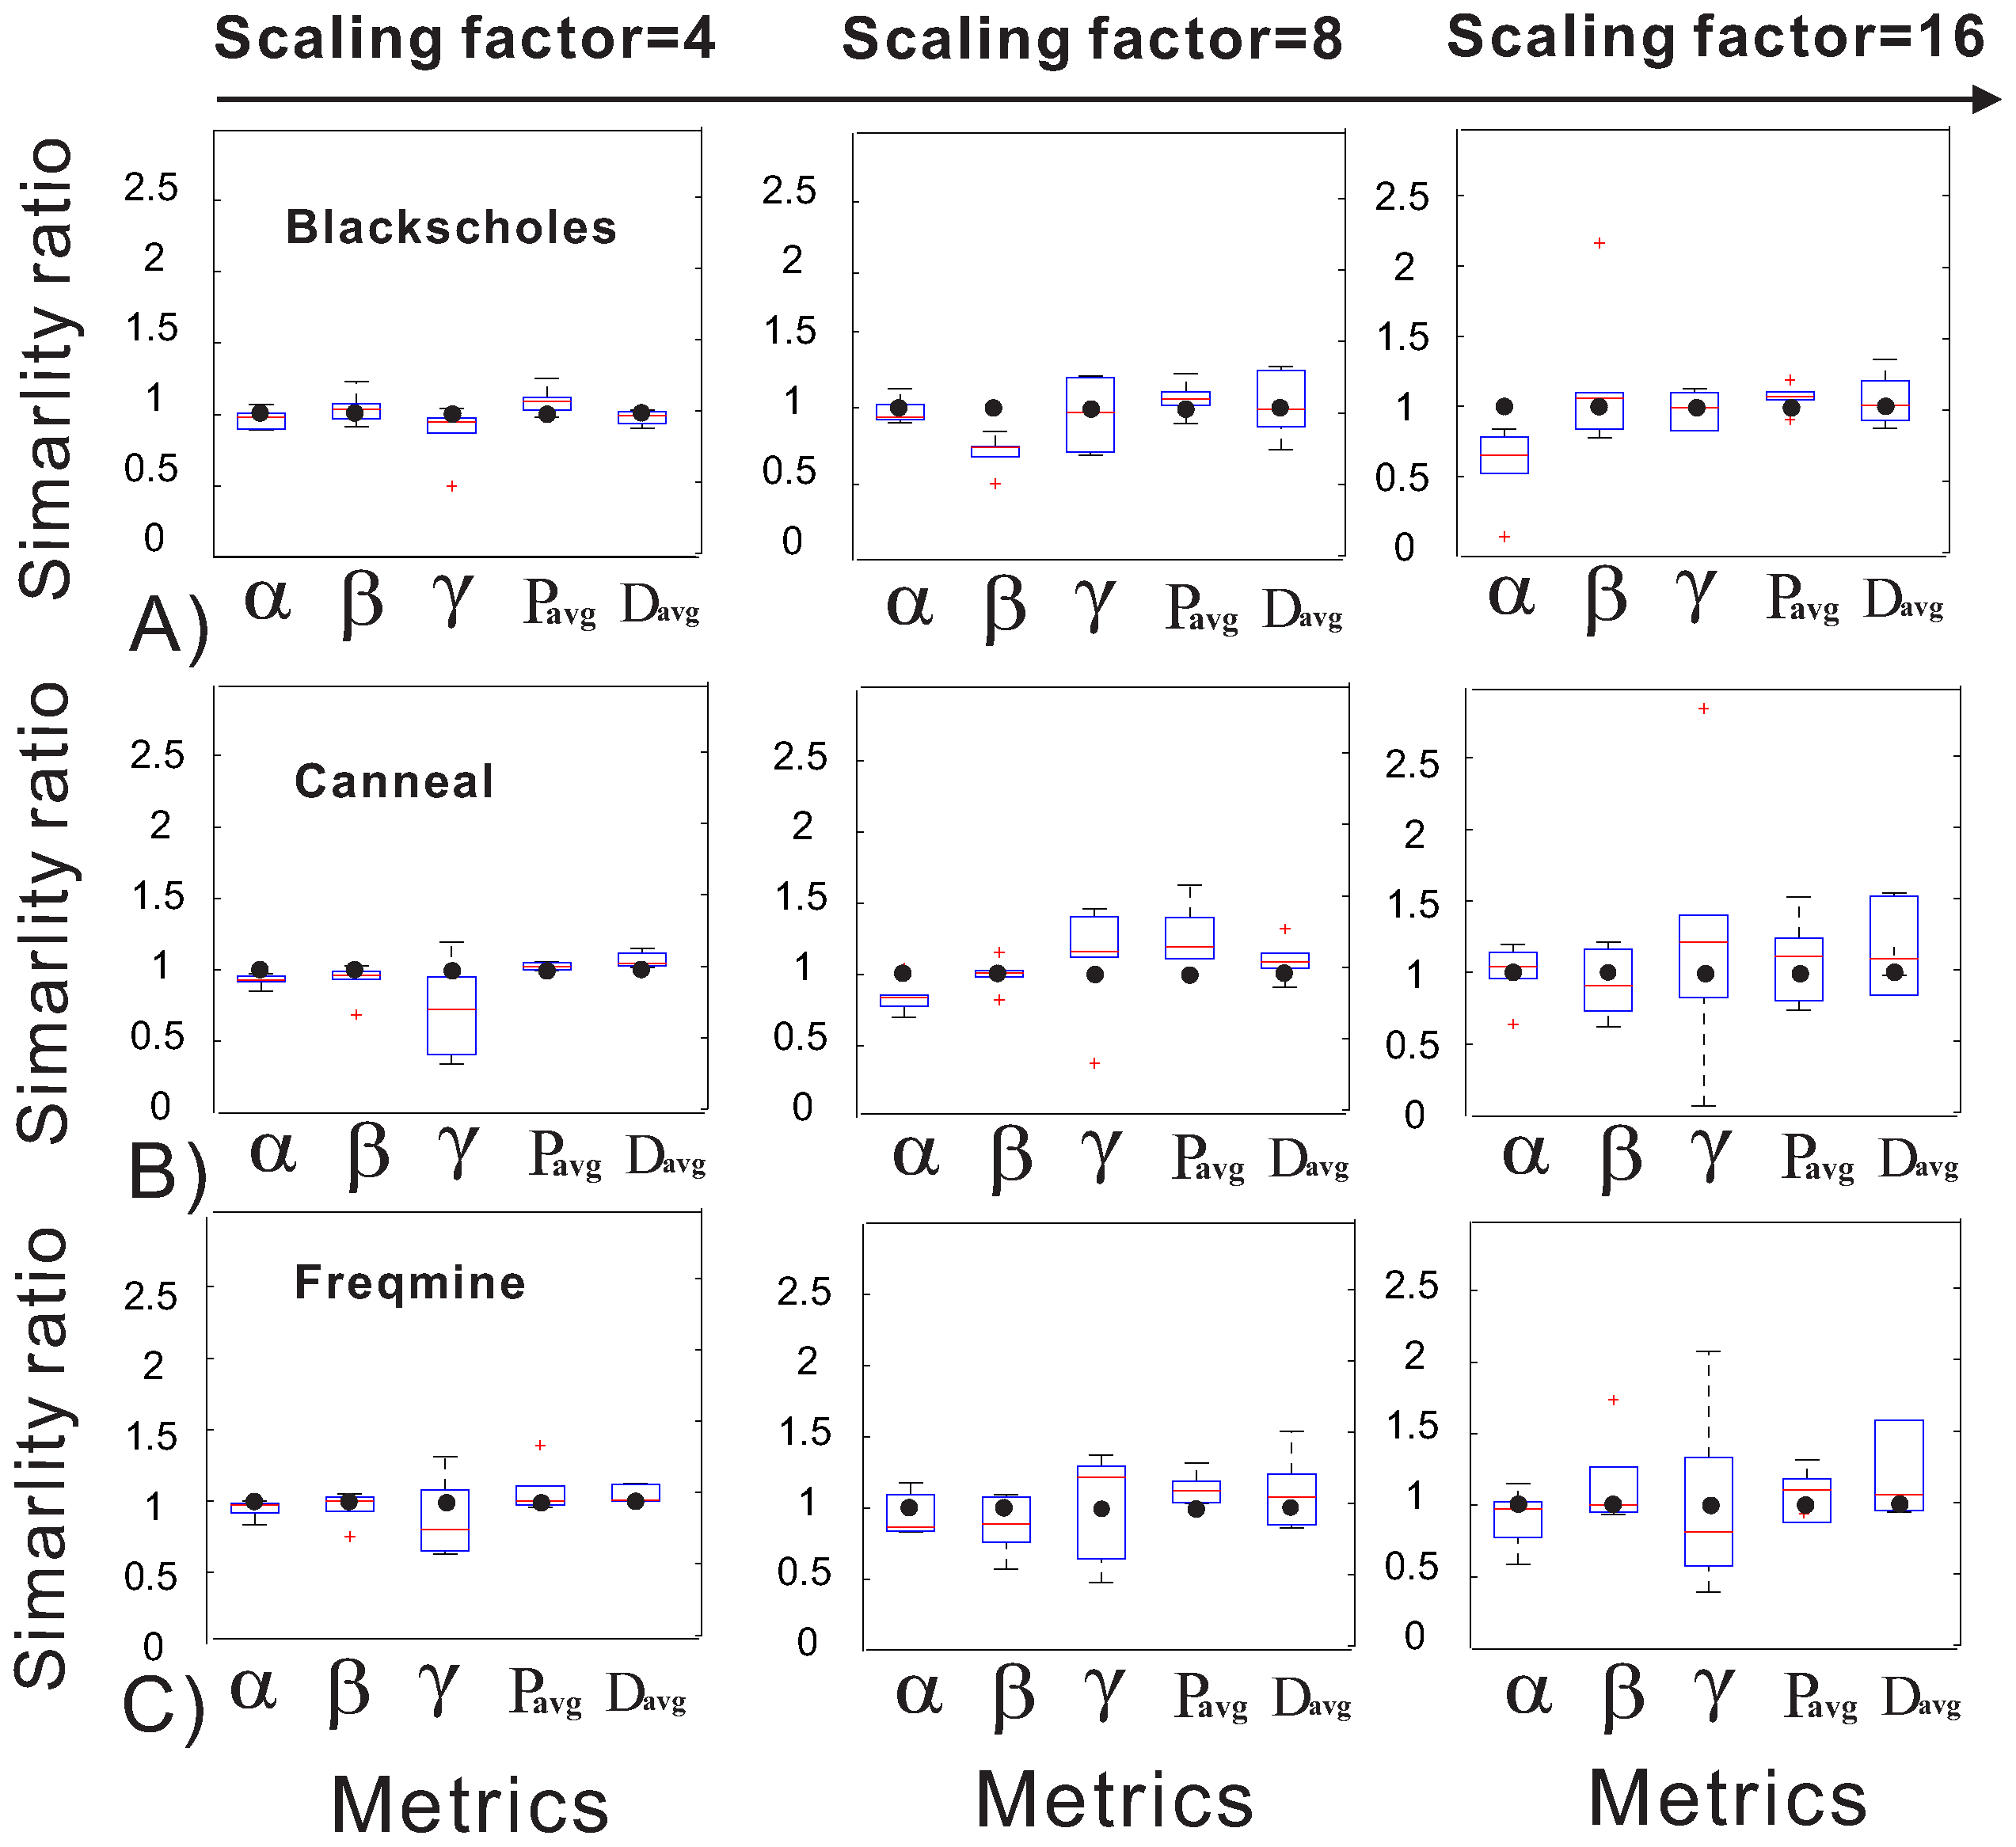
\includegraphics[width=0.8\columnwidth]{str_2.eps}
  \vskip -2mm
  \caption{Measuring structural similarities of graphical models scaled by a factor$= 4,8$ and $16$.}
  \label{fig:stru_sim}
  \vskip -7.5mm
\end{figure}
\indent In the second set of experiments, we would like to check whether the proposed model is able to scale up the application model constructed to an expected scale, meanwhile introducing minimized deviation in the set of interested structural metrics (see Section 4.2). To motivate the  protection of the structural features in a graphical model, not only the proposed model, but in general cases, we should be aware the following fact:  as we mentioned in the previous discussion, the structural characteristics of most of application graphical models, are naturally encoding the spatial dependencies via construction of their geometric structures, i.e., connection of nodes via edges. Actually, prior research efforts in parallelization of algorithms largely rely on the analysis of such structural features and their implications. The change in such structures has significant influence on the execution of the application. Obviously, scaling a graphical model that is able to be used for traffic synthesis is a shortcut to efficiently obtain an array of benchmarks. However, editing the model  arbitrarily might invalidate its applicability to traffic synthesis due to the loss of fidelity. Therefore, we propose the NoC benchmark scaling algorithm based on a complex network theory to obtain new models with expected scales, meanwhile respecting its original structural characteristics. \\
\indent We first constructed the model based on the collected application trace during the ROI phase for all three applications. Then, we use the models as seeds to perform the proposed algorithm. New models are generated with different sets of expected network sizes, i.e., scaling factor$=4, 8$ and $16$. We measured similarity under a set of metrics. The results are reported in Figure~\ref{fig:stru_sim}. For each scaling factor, the measurement is averaged over 100 iterations. Several key observations can be made from the results: i) The proposed algorithm maintains a low level of deviation on average across the set of metrics considered. For a scaling factor of 2, all three graphs stay quite structurally consistent with the original graph. ii) As the scaling factor increases, the average deviation increases due to the structural modification introduced randomly during the refining process. The refining process in the proposed algorithm will randomly connect the newly added node, replicated or randomly introduced, to a existing node in the graph. As the scaling factor goes up, the graph might undergo increased levels of coarsening and refining process, i.e., a "deep-V" process, which boosts the chance of modifications to the graph introduced randomly during the process. Overall, the proposed model can reliably scale the benchmark by at least a factor of 8 and preserving some set of metrics even with a factor of 16.
\section{Summary}
In this work, we have proposed a mathematical framework to synthesize real-world benchmarks that capture spatio-temporal dependencies of the applications. We validate the synthesized traffic through a statistical comparison against the full-system simulation results under real-world application workloads. To allow for the realistic generation of scalable benchmarks that preserve the spatio-temporal dependencies in applications, we have also proposed a NoC benchmark scaling algorithm. The experimental results shows the scaled graphical models are structurally consistent with the original graphs.

\chapter{General Mathematical Framework for Runtime Reconfigurable NoC Synthesis}
\label{cha:ch6}
  \begin{figure}%[htb]
  \centering
  % Requires \usepackage{graphicx}
 % \epsfig{file=t_calc.eps}
  \includegraphics[width=1\columnwidth]{overall_22.eps}
  \vskip -1mm
  \caption{\textbf{Overview of the proposed mathematical framework. The reconfigurable NoC system and its associated applications  are characterized through the proposed system and application graphical models. Then the optimization to the network structural configuration is performed by exploiting the submodular property of the problem. In case of a valid solution does not exist, we introduce the relaxation on problem constraints to obtain a feasible solution while preserve the optimality bound.  } }
  \label{fig:concept}
  \vskip -7mm
\end{figure}

\noindent Workloads induced by real world applications demonstrate strong spatio-temporal variability. Heterogeneous application tasks create inter-coupled traffic patterns with time-varying data and control dependencies exacerbating the workloads requirements running over a large scale NoC-based manycore platform~\cite{bogdan2015mathematical}. For instance, big-data applications like biological simulations~\cite{xue2014disease} usually exhibit high dimensionality in their task structures~\cite{xue_NOCS2014_paper}, which are also varying vastly as a function of widely ranged objectives and unpredictable user input. Consequently, the failure to capture such variations through the development of a best-fit NoC-based system, translates to systems that are prone to computation, communication and power inefficiencies.

\indent To address the spatio-temporal behavior of applications, prior research efforts have focussed on two design methodologies, namely the offline analysis of applications and optimization of application specific NoC architectures and the development of on-line optimization techniques. For instance, application-specific NoC synthesis has been well studied to achieve best-possible performance given a specific application. The synthesis usually generates well optimized NoC configurations and application mappings that are superior to baseline design in terms of energy efficiency and performance \cite{singh2013accelerating}\cite{srinivasan2006linear}, application-specific performance (NoC-based accelerators)\cite{majumder2013high}, reliability \cite{zou2013reliability}, lifetime cost \cite{meyer2010cost}. Such optimization considers one or a subset of applications and captures their traffic pattern and task structures. The synthesis is static with no adaptivity and performed prior to its practical deployment, assuming the application structure is not changing over time. Thus performance is very well optimized if only a fixed set of  applications are considered throughout the life cycle of the platform and the applications are almost temporally homogenous. However, the assumptions made before the synthesis usually do not hold. In reality, it is rarely the case that a dedicated NoC is solely developed for exclusive tasks processing. Instead, the NoC is usually used as fundamental communication infrastructure that integrates a set of heterogeneous processing entities that are expected to run a wide range of applications upon deployment. Most of  applications are very diverse in terms of communication patterns and, more importantly, the traffic patterns are also changing over time. Thus, the statically customized network structure could hardly be a feasible traffic carrier that brings good performance in general cases. 

As an alternative to application specific NoC, the reconfigurable NoCs address this problem by changing their structural features \cite{chen2013smart}\cite{jackson2010skip}, routing algorithm \cite{qian2015fsnoc}, resource management strategy \cite{lee2013adaptive}\cite{kobbe2011distrm}, task assignments \cite{singh2013mapping} to fit to time-varying application requirements. In spite of their successful application in diverse settings, we still lack of a solid theoretical foundation upon which an analytical design methodology could be built to optimize the reconfiguration with optimality guarantees in general cases. Most previous reconfigurable NoCs are proposed, evaluated and validated through a subset of experimental instances without looking at entire problem space from a mathematical perspective. 
%In what follows, we will first formally set up the reconfigurable NoC platform and introduce an array of definitions that help to enrich the model expressivity. Then, as a case study, we will formulate the NoC runtime reconfiguration as optimization problem considering the case where application is characterized through a time-dependent graphical model(e.g., time-varying application task graph or dataflow graph). We will show this optimization problem is NP-hard and prove its \textit{submodularity}. By exploring the submodular property, we propose a greedy heuristics with bounded optimality. 
To address the above-mentioned problems, we propose \textit{a general mathematical modeling framework considering the spatio-temporal characteristics of workloads} and make the following novel contributions:
\begin{itemize}
\item We propose a \textbf{mathematical framework} for capturing the \textbf{dynamic nature} of reconfigurable NoC and applications that enables the formulation of major reconfigurable NoC optimization problems. Our analytical formalism can be applied to arbitrary network topologies and sizes, routing, or heterogeneous resource allocation problems.
\item We illustrate the efficacy of this formalism by formulating the \textbf{NoC reconfiguration as a dynamic optimization problem}. We prove that this optimization is NP-hard and demonstrate that our mathematical formulation satisfies the \textbf{submodularity property} justifying that our proposed greedy based algorithms can attain the optimality region.
\item We evaluate the impact of the proposed mathematical formalism by solving the NoC reconfiguration problem. The experimental results show a $52.3\%$ reduction in network latency, increased capability of handling heavy traffic and $30.2\%$ in energy reduction for our lightweight reconfigurable NoC when compared to baseline design.
\end{itemize}

The paper is organized as follows: In Section II, we formally set up the reconfigurable NoC platform and introduce several definitions that help to enrich the model expressivity. Section III presents a case study of the NoC runtime reconfiguration problem considering the case where application is characterized through a time-dependent graphical model (e.g., time-varying application graph). We show this optimization problem is NP-hard and prove its \textit{submodularity}. By exploiting the submodularity property, we propose greedy heuristics with bounded optimality. Sections IV and V summarize our experimental results and our main achievements.

\section{Mathematical Modeling and Optimization Framework}
\subsection{Architectural Modeling Framework}
\noindent \textbf{Definition 1:}\label{def:noc} \textit{A \textbf{reconfigurable network-on-chip} (NoC) is defined as a \textbf{connected dynamic directed graph} $G(t)=(N(t),E(t);\gamma(t),\mathcal C)$ at time $t$, where $n_{i} \in N(t)$ is a tile and represents a collection of functional units, and $E(t)$ denotes the collection of physical links between different nodes in $N(t)$. The $e_{i,j} \in E(t)$ denotes the link from $n_{i}$ to $n_{j}$.}

We should note that $N(t)$ is the set of enabled network functional units (e.g.,  DSPs, general processors, customized processing elements, memories or communication transceivers). The composition of $N(t)$ can change as the subset of nodes are enabled or disabled over time. Also, the reconfigurable NoC usually takes advantage of different switching techniques for best possible performance under diverse workloads.  Therefore, $e_{i,j}$ could be a regular link between two routers or a direct link established between tiles without interfacing with routers. To distinguish between regular and circuit links, we introduce the following definition:

\noindent \textbf{Definition 2:}{ \textit{Edge $e_{i,j}$ is a \textbf{circuit link} if there exists a direct link from $n_{i}$ to $n_{j}$ that allows circuit switching. $E(t)$ induces a function $\mathcal I: E(t) \rightarrow R$ such that $e_{i,j}$ is a circuit link if and only if $\mathcal I(e_{i,j})=1$}.}\label{def:circuit}

The circuit switching link is set up in the regular network to improve throughput over critical traffic path in reconfigurable NoCs.  Circuit switching reserves the entire bandwidth of the dedicated link and skips all routing stages, thus improving greatly the communication throughput when used between a pair of nodes. By connecting different circuit links together, it is possible for a subset of nodes to communicate over such dedicated circuit links for faster data exchange. To characterize such collection of nodes, we introduce the circuit component concept as follows:

\noindent \textbf{Definition 3:}{ \textit{A subset $N'(t) \subseteq N(t)$ is a \textbf{circuit component} $\mathcal T$ if and only if for any pair of nodes $ n_i$ and $n_j \in N'(t)$, there exists a circuit link between them.}\label{def:circuit_component}

A circuit component $\mathcal T$ in $G(t)$ forms a connected subgraph enabling data transfer over dedicated links with augmented bandwidth and reduced latency. For example, %a trivial circuit component is just a single node and 
the simplest circuit component is a pair of nodes with a direct link that skips the routers at both ends. Generally speaking, the reconfiguration of NoC can be viewed as a process of enabling circuit components in the regular network to provide express ways for critical data transmission. 

\noindent \textbf{Definition 4:}{ The \textit{$\gamma(t): N(t) \times N(t) \rightarrow G(t)$ is the \textbf{routing function} at time $t$ that maps a pair of nodes $n_{i}$ and $n_{j}$ to a subgraph $G'(t)$ of $G(t)$ such that: i) $n_{i},n_{j} \in G'(t)$ and ii) there exists at least a path from $n_i$ to $n_j$. } 

\noindent Of note, the $(N(t),E(t);\gamma(t))$ forms a 3-tuple that defines a regular NoC without reconfiguration  features, where $N(t)$ and $E(t)$ characterize its structural properties. $\gamma(t)$ denotes all possible paths for data exchange. 
\begin{figure}%[htb]
  \centering
  % Requires \usepackage{graphicx}
 % \epsfig{file=t_calc.eps}
  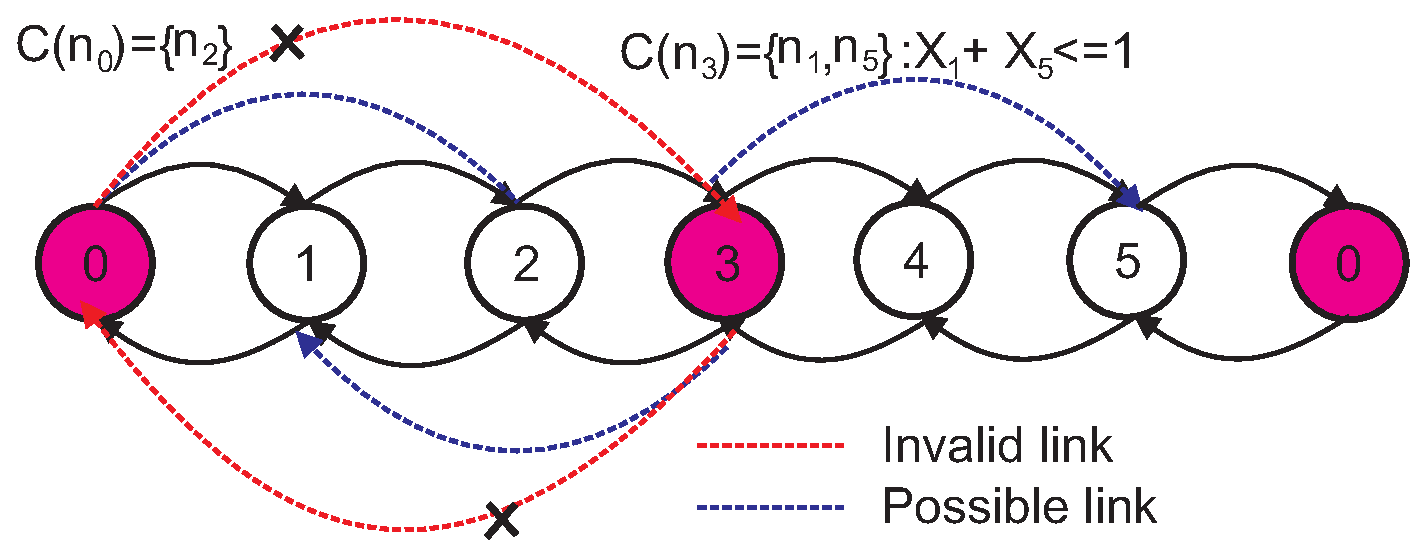
\includegraphics[width=0.8\columnwidth]{alter_set.eps}
  \vskip -1mm
  \caption{\textbf{Augmented connectivity sets are shown for $n_{0}$ and $n_{3}$. $n_{3}$ is configurable to set up link with $n_1$ and $n_5$ whereas both links can not be established at the same time. Similar link to $n_0$ is invalid due to physical limitation.} }
  \label{fig:augment}
  \vskip -6mm
\end{figure}

To be able to model and express the reconfiguration capability, we define the \textit{augmented connectivity function} $\mathcal C$:

\noindent \textbf{Definition 5:} \textit{ $\mathcal C: N(t)\rightarrow 2^{N(t)} $ is the \textbf{augmented connectivity function} (ACF) that associates each node $n_{i} \in E(t)$ at time $t$ with a subset of nodes $\mathcal C(n_{i})=\{n_{j}|n_{j} \in N(t)\}$, to which $e_{i,j}$ could be possibly set up. The set $\mathcal C(n_{i})$ is called \textbf{augmented connectivity set} (ACS).}

By definition, $\mathcal C(n_{i})$ denotes all the possible links that could be alternatively established for $n_{i}$ other than the current links in $\{e_{i,j}|e_{i,j} \in E(t)\}$. We should note that the detailed form of $\mathcal C$ and its range are limited by the physical constraints in a specific architecture. For instance in Figure \ref{fig:augment}, a physical link can not be inserted between $n_3$ and $n_0$ that are too far away from each other given physical limitations (e.g., propagation delay should be less than one cycle). Moreover, a link might not be set up from $n_i$ to $n_{j}$ even if $n_{j} \in \mathcal C(n_i)$. Such constraint comes mostly from architectural limitations which forbid some links from being set up simultaneously  as shown in Figure \ref{fig:augment}. To consider such cases, we introduce a set of constraints associated with $\mathcal C(n_i)$. Let $X_{j}$ be a binary variable such that $X_{j}=1$ if $n_{j} \in \mathcal C(n_i)$ and $e_{i,j}$ is set up. Otherwise, $X_{j}=0$.
\begin{equation}\label{eq:C_constr}
\Sigma \alpha_{j}X_{j}\leq K 
\end{equation}
where, $\alpha_{j} \in \{0,1\}$ represents whether $X_{j}$ is masked or not in the constraints. $K \in \mathcal N$ denotes the maximum number of links that can be established simultaneously. Equation~\eqref{eq:C_constr} defines a constraint, which encodes the physical limitation that a subset of nodes in $\mathcal C(n_i)$ can not connect to $n_i$ at the same time. By changing the configuration of $\{\alpha_{j}\}$, eq.~\eqref{eq:C_constr} forms an array of constraints that capture all such physical limitations.  Thus, we can define the reconfigurable NoC in the general case:

\noindent \textbf{Definition 6 (reconfigurability):} \textit{A node $n_{i}$ is reconfigurable if and only if $C(n_i) \neq \emptyset$. An NoC system $G(t)=(N(t),E(t);\gamma(t),\mathcal C)$ is reconfigurable at time $t$ if there exists at least one node $n_i \in N(t) $ that is reconfigurable.}

\noindent Definition 6 formally defines the reconfigurability. An NoC system $G(t)$ is reconfigurable as long as any one of its nodes has non-empty ACS. By picking up nodes from ACS and constructing new edges over time, $E(t)$ evolves as a function of reconfiguration decisions made prior to time $t$. Of note, Definition 1 enforces the connectivity of a given NoC system. Therefore, the routing algorithm $\gamma(t)$ will also change accordingly to guarantee all the nodes are reachable. Combined with the dynamics of $N(t)$, $G(t)=(N(t),E(t);\gamma(t),\mathcal C)$ describes a dynamical system with time-varying structural characteristics, i.e., $N(t)$, $E(t)$ and $\gamma(t)$, driven by the reconfiguration decisions made upon $\mathcal C(n_i)$ over time. By introducing attributes of interest and associating them with $G(t)$ and application tasks, we are able to construct the theoretical basis on which general NoC reconfiguration could be formulated as optimization problems. To provide an illustrative example of this framework, we present the runtime NoC reconfiguration optimization problem given time-dependent workloads characterized by graphical models.
\subsection{Application Modeling Framework}
Generally speaking, any runtime NoC reconfiguration is an optimization process that searches for the best-fit network structural configurations and application task assignments (i.e, mapping of tasks to specific tiles), given an objective function and a set of constraints. In contrast to application-specific NoC synthesis, runtime optimization is an online process repeatedly synchronized with the time-dependent characteristics of the running applications. This process usually consists of two phases: an execution phase and an optimization phase. In the optimization phase, the optimization will take the profile of applications as input and decide on a best possible network configuration for the execution phase. Profiling the application is a very complex research topic and several models were developed in different contexts. A detailed discussion is beyond the scope of this work. Next, we consider profiling applications via graphical models although the proposed NoC system model $G(t)$ has no constraints on profiling techniques.

\noindent \textbf{Definition 7:}\label{def:app} \textit{ An application $\mathcal A(t)$ is a \textbf{dynamical directed graph} $\mathcal A(t)=(V(t),C(t);\mathcal P(\Sigma,\mathcal F))$ at time $t$. Each vertex $v_{i} \in V(t)$ is a task of the application. $c_{i,j} \in C(t)$ represents a directed data/control dependency from task $v_i$ to task $v_{j}$. }
 
Each application $\mathcal A(t)$ induces a profiling system $\mathcal P(\Sigma,\mathcal F)$. $\Sigma$ is the finite functionality alphabet given specific application context. It contains symbols that characterize the functionality of interest. Functionality profiling function $\mathcal F:V \rightarrow 2^{\Sigma}$ relates each task $v_{i}$ of $\mathcal A(t)$ at time $t$ with a finite set of symbols defined in $\Sigma$ as functionality requirement set $\mathcal F(v_{i})$. To provide some intuition, $\Sigma$ can be as simple as an integer set $\{0,1,2,3\}$ in context of numeric computation where $2$ and $3$ represent ``addition" and ``multiplication". $0$ and $1$ represent ``integer" and ``floating-point", respectively. $\mathcal F$ will induce a functionality requirement set for each node $v_i$. A node $v_i$ with $\mathcal F(v_i)=\{1,2,3\}$ requires floating-point addition and multiplication operations, while a node $v_j$ with $\mathcal F(v_j)=\{0,2\}$ requires only integer addition. By changing alphabet $\Sigma$ based on application context, i.e., application task profiled with interested details, $\mathcal P(\Sigma,\mathcal F)$ is able to characterize each task with sufficiently many mathematical details.

Moreover, we will use the same profiling system $\mathcal P(\Sigma,\mathcal F)$ to characterize the ``capabilities" of each tile $n_{i} \in G(t)$ such that we can easily compare capabilities of the NoC $G(t)$ with the functionality requirements from the application domain. This constitutes the foundation for application task assignment. For each $n_{i}$ of $G(t)$, we define $\mathcal F(n_i)$ as capability set such that, an application task $v_{i}$ with functionality requirement set $\mathcal F(v_i)$ can be mapped to $n_i$ \textit{only if} $\mathcal F(v_i) \subseteq \mathcal F(n_i)$. 
 
Each directed edge $c_{i,j} \in C(t)$ is characterized by a data generation process $P_{c_{i,j}}(k,t)=P\{\mathcal N(t)=k,k \in N\}$ where $\mathcal N(t)$ is a counting process which denotes the number of packets generated in time interval $[t,t+\tau]$. $P_{c_{i,j}}(k,t)$ captures the time-varying behavior of the application. To provide some intuition, the data generation process could be a Poisson process if no memory-effect is present or it could be a fractal process governed by power-laws exhibiting long-range memory \ dependency. Therefore, for an execution phase of length $T$, the \textit{average traffic volume} $q(c_{i,j})$ from task $v_i$ to task $v_j$ could be calculated as follows,
\begin{equation}\label{eq:traffic_vol}
q(c_{i,j})=\int_{t}^{t+T} \int_{-\infty}^{\infty} kP_{c_{i,j}}(k,t) dk dt
\end{equation}

We define by $b(c_{i,j})$ the minimal bandwidth requirement for communication from $v_{i}$ to $v_{j}$. It should be noted that this requirement comes from the execution time constraints posed by the associated tasks. We define $\mathcal B(e_{i,j}, \mathcal I(e_{i,j}))$ as the bandwidth provided by the link $e_{i,j} \in E(t)$ given NoC system $G(t)$. Attribute $\mathcal I(e_{i,j})$ is introduced in $\mathcal B$ to consider the bandwidth difference between regular and circuit links. We check the validity of assigning a task to one tile in NoC system by comparing the functionality requirement and capability set, a pair of tasks $v_i$, $v_j$ can be mapped to $n_i$ and $n_j$ \textit{only if} $b(c_{i,j}) \leq B(e_{i,j}, \mathcal I(e_{i,j}))$ and $b(c_{j,i}) \leq B(e_{j,i}, \mathcal I(e_{j,i}))$. 

\subsection{Runtime Reconfiguration Problem Formulation}

Based on the mathematical description of the reconfigurable NoC and the application, the runtime NoC reconfiguration is performed in optimization phase by modifying the structural properties of $G(t)$, i.e., changing the $E(t)$ and constructing circuit components $\mathcal T$, based on ACF $\mathcal C$ given application $\mathcal A(t)$ and execution phase horizon $T$. To formally state the optimization problem, we first introduce the definition of \textit{compatible partition} of an application $\mathcal A(t)$ given $G(t)$. Let $\pi=\{\pi_1, \ldots, \pi_n\}$ be a partition of a given application $\mathcal A(t)=(V(t),C(t);\mathcal P(\Sigma,\mathcal F))$ such that,
 
\noindent \textbf{Definition 8:} \textit{The partition $\pi$ is \textbf{compatible} with NoC system $G(t)=(N(t),E(t);\gamma(t),\mathcal C)$ at time $t$ if and only if for any partition element $\pi_{k}$ there exists a circuit component $\mathcal T_{k}$ in $G(t)$ such that,}
\begin{equation}\label{eq:compt_1}
\cup_{v_i \in \pi_{k}} \mathcal F(v_i) \subseteq \cup_{n_i\in \mathcal T_{k}} \mathcal F(n_i),
\end{equation}
\begin{equation}\label{eq:compt_2}
|\pi_k| \leq |\mathcal T_{k}|
\end{equation}
\begin{equation}\label{eq:compt_3}
\mathcal T_{i} \cap \mathcal T_{j}=\emptyset, \forall i\neq j
\end{equation}

By definition 8, the reconfiguration optimization process can be understood as a searching process wherein a compatible partition $\pi$ can be found such that $G(t)$ is also partitioned by corresponding circuit components, which cover maximum number of overall traffic volume. Alternatively stated, the reconfiguration objective is to adapt the NoC structure to provide maximum bandwidth, i.e., the dedicated traffic path, to maximum possible share of traffic. Constraint \eqref{eq:compt_1} represents a sanity check which guarantees that the circuit component $\mathcal T_{k}$ to which the subset of tasks in $\pi_{k}$ are assigned, covers all functionalities required to execute them. Constraint \eqref{eq:compt_2} indicates the computing resources within $\mathcal T_{k}$ can not be shared at the same time. Constraint \eqref{eq:compt_3} induces a one-to-one assignment between a partition element $\pi_{k}$ and a circuit component $\mathcal T_{k}$.

To quantify the bandwidth gain due to adoption of circuit components, we introduce \textit{intra-component bandwidth factor} $f_{a}(\mathcal T{i})$ and \textit{inter-component bandwidth factor} $f_{r}(\mathcal T{i},\mathcal T{j})$. The $f_{a}$ represents the ratio between the bandwidth of circuit link and regular link. The $f_{r}$ is defined as follows:
\begin{equation}\label{eq:fr}
f_r(\mathcal T{i},\mathcal T{j})=\frac{\mathcal O(\mathcal T{i},\mathcal T{j})}{\mathcal D(\mathcal T{i},\mathcal T{j})}
\end{equation}
where $\mathcal O(\mathcal T{i},\mathcal T{j})$ represents the number of non-overlapping links of all possible paths from $\mathcal T_{i}$ to $\mathcal T_{j}$, the $\mathcal D(\mathcal T{i},\mathcal T{j})$ is the Manhattan distance from $\mathcal T_{i}$ to $\mathcal T_{j}$, which is calculated by the minimum Manhattan distance from any node $n_i \in \mathcal T{i}$ to any node $n_j \in \mathcal T_{j}$, the $f_{r}$ gives an upper bound for bandwidth gain assuming data can be promptly exchanged within a circuit component such that all paths between two circuit components can be used simultaneously to send the data and, the data will be gathered from those paths at the destination node with no cost. Thus, we can formulate the runtime NoC reconfiguration problem as follows:

\noindent\textbf{\textit{Runtime NoC reconfiguration -- primal problem formulation:}}

\noindent\textbf{Given} a reconfigurable NoC system $G(t)=(N(t),E(t);\gamma(t),$\\$\mathcal C)$, an application $\mathcal A(t)=(V(t),C(t);\mathcal P(\Sigma,\mathcal F))$ at time $t$ and execution phase horizon $T$,

\noindent\textbf{Find} a  partition $\pi$ of $\mathcal A(t) $ and the corresponding circuit components $\{ \mathcal T_{k}\}$ that minimize following cost function:
\begin{equation}\label{eq:problem_form}
\min\limits_{\pi,\mathcal T} \sum_{\mathcal T_{i}} \sum_{\mathcal T_{j}\neq \mathcal T_{i}} (\frac{q(\mathcal T_{i},\mathcal T_{j})}{f_r(\mathcal T{i},\mathcal T{j})}+\lambda(\mathcal D(\mathcal T{i},\mathcal T{j})(E_{s}+E_{l}))q(\mathcal T_{i},\mathcal T_{j}))
\end{equation}
\noindent\textbf{Subject to:} Partition $\pi$ is compatible.

\noindent Of note, the $q(\mathcal T_{i},\mathcal T_{j})$ is the sum of average traffic volume from $\mathcal T_{i}$ to $\mathcal T_{j}$ given the length of execution phase $T$. The $q(\mathcal T_{i},\mathcal T_{j})$ is calculated as the sum of traffic volume from all the nodes in $\mathcal T_{i}$ to all the nodes in $\mathcal T_{j}$, given $\pi_{k}$ and $\pi_{l}$ are assigned to them, respectively. The summation in the objective function \eqref{eq:problem_form} is decided by two terms that consider the efficiency of communication and energy, respectively. The communication efficiency is quantified by how much traffic is left with no dedicated link to use (i.e., $q(\mathcal T_{i},\mathcal T_{j})$) and how well the traffic can be delivered (i.e., $f_{r}(\mathcal T{i},\mathcal T{j})$). Ideally, the first term is zero when either all traffic use the dedicated communication bandwidth or there exist infinite number of non-overlapping traffic paths between two circuit components. $E_{s}$ is the switching energy in a router and $E_{l}$ is traversing energy per hop. $\mathcal D(\mathcal T{i},\mathcal T{j})$ is the Manhattan distance from $\mathcal T_{i}$ to $\mathcal T_{j}$. Thus, the second term calculates the overall energy consumption of all inter-component traffic that travels over regular links. $\lambda$ is a tuning parameter decided in experiments, which balances the contribution of these two terms.

The objective function \eqref{eq:problem_form} seeks to guide the reconfiguration of the NoC structure given current application workload such that, the number of circuit components is maximized to sustain the traffic requirements while also improving the energy efficiency, i.e., the dedicated links provide superior bandwidth and reduce energy consumption by skipping multiple routing stages. Next, we show that this problem is NP-hard and propose a greedy algorithm that solves the problem while also considering the convergence guarantees to the optimality.

\subsection{Complexity and Algorithm Analysis}

\noindent\textbf{\textit{Theorem 1:}} The runtime NoC reconfiguration problem described in \eqref{eq:problem_form} is NP-hard.\hfill $\diamond$

\noindent\textbf{\textit{Proof:}} The proof follows by noticing that there exists an NoC system $G(t)=(N(t),E(t);\gamma(t),$$\mathcal C)$ that, for any partition $\pi$ of $\mathcal A(t)$, it is compatible. Therefore, the problem reduces to a quadratic assignment problem, that is NP-hard, between partition $\{\pi_k\}$ and circuit components $\{\mathcal T_{k}\}$ that minimizes ~\eqref{eq:problem_form}. Because~\eqref{eq:problem_form} contains (as subclass of problems) one that is NP-hard, it follows that \eqref{eq:problem_form} is also NP-hard.

Next, we show the feasibility space of \eqref{eq:problem_form} given by the compatibility constraint, see Definition 8,  is \textit{submodular}. To prove the optimization problem  \eqref{eq:problem_form} is submodular, it should be noted that \eqref{eq:problem_form} could be equivalently defined as its dual maximization problem as:

\noindent\textbf{\textit{Runtime NoC reconfiguration -- dual problem formulation:}}

\noindent\textbf{Given} a reconfigurable NoC system $G(t)=(N(t),E(t);\gamma(t),$\\$\mathcal C)$, an application $\mathcal A(t)=(V(t),C(t);\mathcal P(\Sigma,\mathcal F))$ at time $t$ and execution phase horizon $T$.\\
\noindent\textbf{Find} a  partition $\pi$ of $\mathcal A(t) $ and corresponding circuit components $\{ \mathcal T_{i}\}$ that maximize the following cost function:
\begin{equation}\label{eq:problem_form_2}
\max\limits_{\pi,\mathcal T} \sum_{\mathcal T_{i}}( f_{a}(\mathcal T_{i})\frac{q(\mathcal T_{i})}{q_{\Sigma}}+ \frac{1}{\lambda} E_{\Delta}(\mathcal T_{i}) )
\end{equation}
\noindent\textbf{Subject to:} Partition $\pi$ is compatible.

Of note, the $q(\mathcal T_{i})$ is the overall traffic volume in $\mathcal T_{i}$ and $q_{\Sigma}$ denotes overall traffic volume of $\mathcal A(t)$ given execution phase horizon $T$. The $f_{a}(\mathcal T_{i})$ is the intra-component bandwidth factor, i.e., ratio of bandwidth between circuit link and regular link. Thus, the first term in the summation considers the bandwidth gain obtained by assigning dedicated circuit link to application workloads. $E_{\Delta}(\mathcal T_{i})$ represents the amount of energy saved by using dedicated links for traffic $q(\mathcal T_{i})$, compared to the energy consumed by using regular link instead. $E_{\Delta}(\mathcal T_{i})$ depends on how each task in $\mathcal A(t)$ is assigned to tiles in $G(t)$.

\noindent\textbf{\textit{Lemma 1:}} The runtime NoC reconfiguration objective function described in \eqref{eq:problem_form_2} is \textit{submodular}.\hfill $\diamond$\\
\textbf{\textit{Proof:}} Given an application partition $\pi$, let us define two compatible circuit component sets $\mathcal T_A \subseteq \mathcal T_B$ where $\mathcal T_A$ or $\mathcal T_B$ is a collection of circuit components that are compatible with a subset of partition elements in $\pi$. Let $\mathcal T_{e} \in \mathcal T$ be an arbitrary circuit component to which a partition $\pi_{k}$ will be assigned. We denote $\mathcal G(\mathcal T_A)$ as the objective function defined in \eqref{eq:problem_form_2} given $\mathcal T_A$. Thus, if $\mathcal T_{e} \notin \mathcal T_{B}$,
\begin{equation}\label{eq:submodular}
\mathcal G(\mathcal T_A \cup \mathcal T_e)-\mathcal G(\mathcal T_A )= f_{a}(\mathcal T_{e})\frac{q(\mathcal T_{e})}{q_{\Sigma}}+ \frac{1}{\lambda} E_{\Delta}(\mathcal T_{e}) 
\end{equation}
\begin{equation}\label{eq:submodular_2}
\mathcal G(\mathcal T_B \cup \mathcal T_e)-\mathcal G(\mathcal T_B )= f_{a}(\mathcal T_{e})\frac{q(\mathcal T_{e})}{q_{\Sigma}}+ \frac{1}{\lambda} E_{\Delta}(\mathcal T_{e}) 
\end{equation}
Otherwise, if $\mathcal T_{e} \in \mathcal T_{B}$, $\mathcal G(\mathcal T_B \cup \mathcal T_e)-\mathcal G(\mathcal T_B )=0$. Therefore, 
\begin{equation}\label{eq:submodular_2}
\mathcal G(\mathcal T_B \cup \mathcal T_e)-\mathcal G(\mathcal T_B )\leq G(\mathcal T_A \cup \mathcal T_e)-\mathcal G(\mathcal T_A )   \end{equation}
holds for  any $\mathcal T_A \subseteq \mathcal T_B \subset \mathcal T$ and $\mathcal T_{e} \in \mathcal T$. Hence, the objective function \eqref{eq:problem_form_2} is submodular. Moreover, eq. \eqref{eq:submodular} shows $\mathcal G$ is also monotonic.

\noindent For \textit{monotonic submodular} functions\cite{nemhauser1978best}, we have the following theorem,\\
\textbf{\textit{Theorem 2:}} 
Given a monotonic submodular function $\mathcal G$, $G(\emptyset)=0$, the greedy maximization algorithm returns:
\begin{equation}\label{eq:max}
 \mathcal G(\pi, \mathcal T_{greedy}) \geq (1-1/e) \max\limits_{|\mathcal T|\leq N}G(\pi,\mathcal T)
\end{equation}
where $N$ is maximum number of circuit components that are possibly constructed. Thus, even though the runtime NoC reconfiguration problem is NP-hard, we can propose a greedy heuristic Alg. \ref{alg:maximization} with guaranteed optimality. In Algorithm \ref{alg:maximization}, $G(t)$ and $\mathcal A(t)$ are first constructed for an execution phase of length $T$. Then the algorithm will partition the application $\mathcal A(t)$ constrained by the physical limitations posed by $G(t)$ such that the maximum possible amount of traffic is covered within all partition components $\{\pi_{k}\}$, i.e., the cut weight is minimal. We assume the Fiduccia-Mattheyses algorithm~\cite{fiduccia1982linear} that is able to handle unbalanced partitions. The physical limitations majorly prevent infeasible partitions. A partition is considered infeasible if any of its partition components is beyond a predefined size such that no compatible circuit component is possibly found, see Definition 8, \eqref{eq:compt_1}, \eqref{eq:compt_2}, and \eqref{eq:compt_3}. Then a greedy heuristic will construct a circuit component $T_{e}$ that maximizes the incremental gain of $\mathcal G$ and add it to $\mathcal T$. The cycle repeats until $\pi$ is compatible. 

Algorithm \ref{alg:maximization} returns a solution to \eqref{eq:problem_form_2} with bounded optimality as long as it exists. Otherwise, i.e., no circuit components can be constructed to be compatible with given partition, or it takes indefinite time to reach one, Algorithm \ref{alg:maximization} might practically fail. To obtain an approximated solution in such cases, we propose a relaxation process.

\noindent \textbf{Definition 9:}\label{def:relax_1} \textit{ An \textbf{$l$-relaxed circuit component} is a subset of nodes $N'(t) \subset N(t)$ if and only if for any pair of nodes $n_i$, $n_j$, there exists a link $e_{i,j}$ between them such that,  at most $l$ of all such links are regular links.}

\noindent \textbf{Definition 10:}\label{def:relax_2} \textit{ Partition $\pi$ is \textbf{$l$-compatible} with NoC system $G(t)=(N(t),E(t);\gamma(t),\mathcal C)$ at time $t$ if and only if for any partition element $\pi_{k}$ there exists a l-relaxed circuit component $\mathcal T_{i}$ in $G(t)$ such that \eqref{eq:compt_1}, \eqref{eq:compt_2}, and \eqref{eq:compt_3} are met. }

The definitions 9 and 10 set the relaxation on the concepts of circuit component and compatible partition. Ideally, we reconfigure the NoC structures to fit the application workloads with the hope that all traffic paths are able to exploit their dedicated bandwidth, i.e., circuit links. However, there is a chance that such circuit links are difficult to construct given architectural and physical constraints. Therefore, we need to relax the Definition 8 in such cases, while still requiring a link to exist between any pair of nodes, to allow some of such links to be regular links. Definition 9 generalizes the circuit component such that not only the dedicated links, i.e., circuit link, but also the express links , i.e., one-hop regular links between routers, are considered. Thus, the constraint for \eqref{eq:problem_form_2} could be relaxed to $l$-compatible as stated by Definition 10. It is noted that the relaxation on the constraint does not affect the submodularity of $\mathcal G$, thus the optimality bound in \eqref{eq:max} holds.

 In what follows, we will instantiate a reconfigurable NoC architecture as optimization case study to evaluate the efficacy of the proposed mathematical framework with realistic workloads characterized by graphical models.

\begin{figure}[tb]
  \centering
  % Requires \usepackage{graphicx}
 % \epsfig{file=t_calc.eps}
  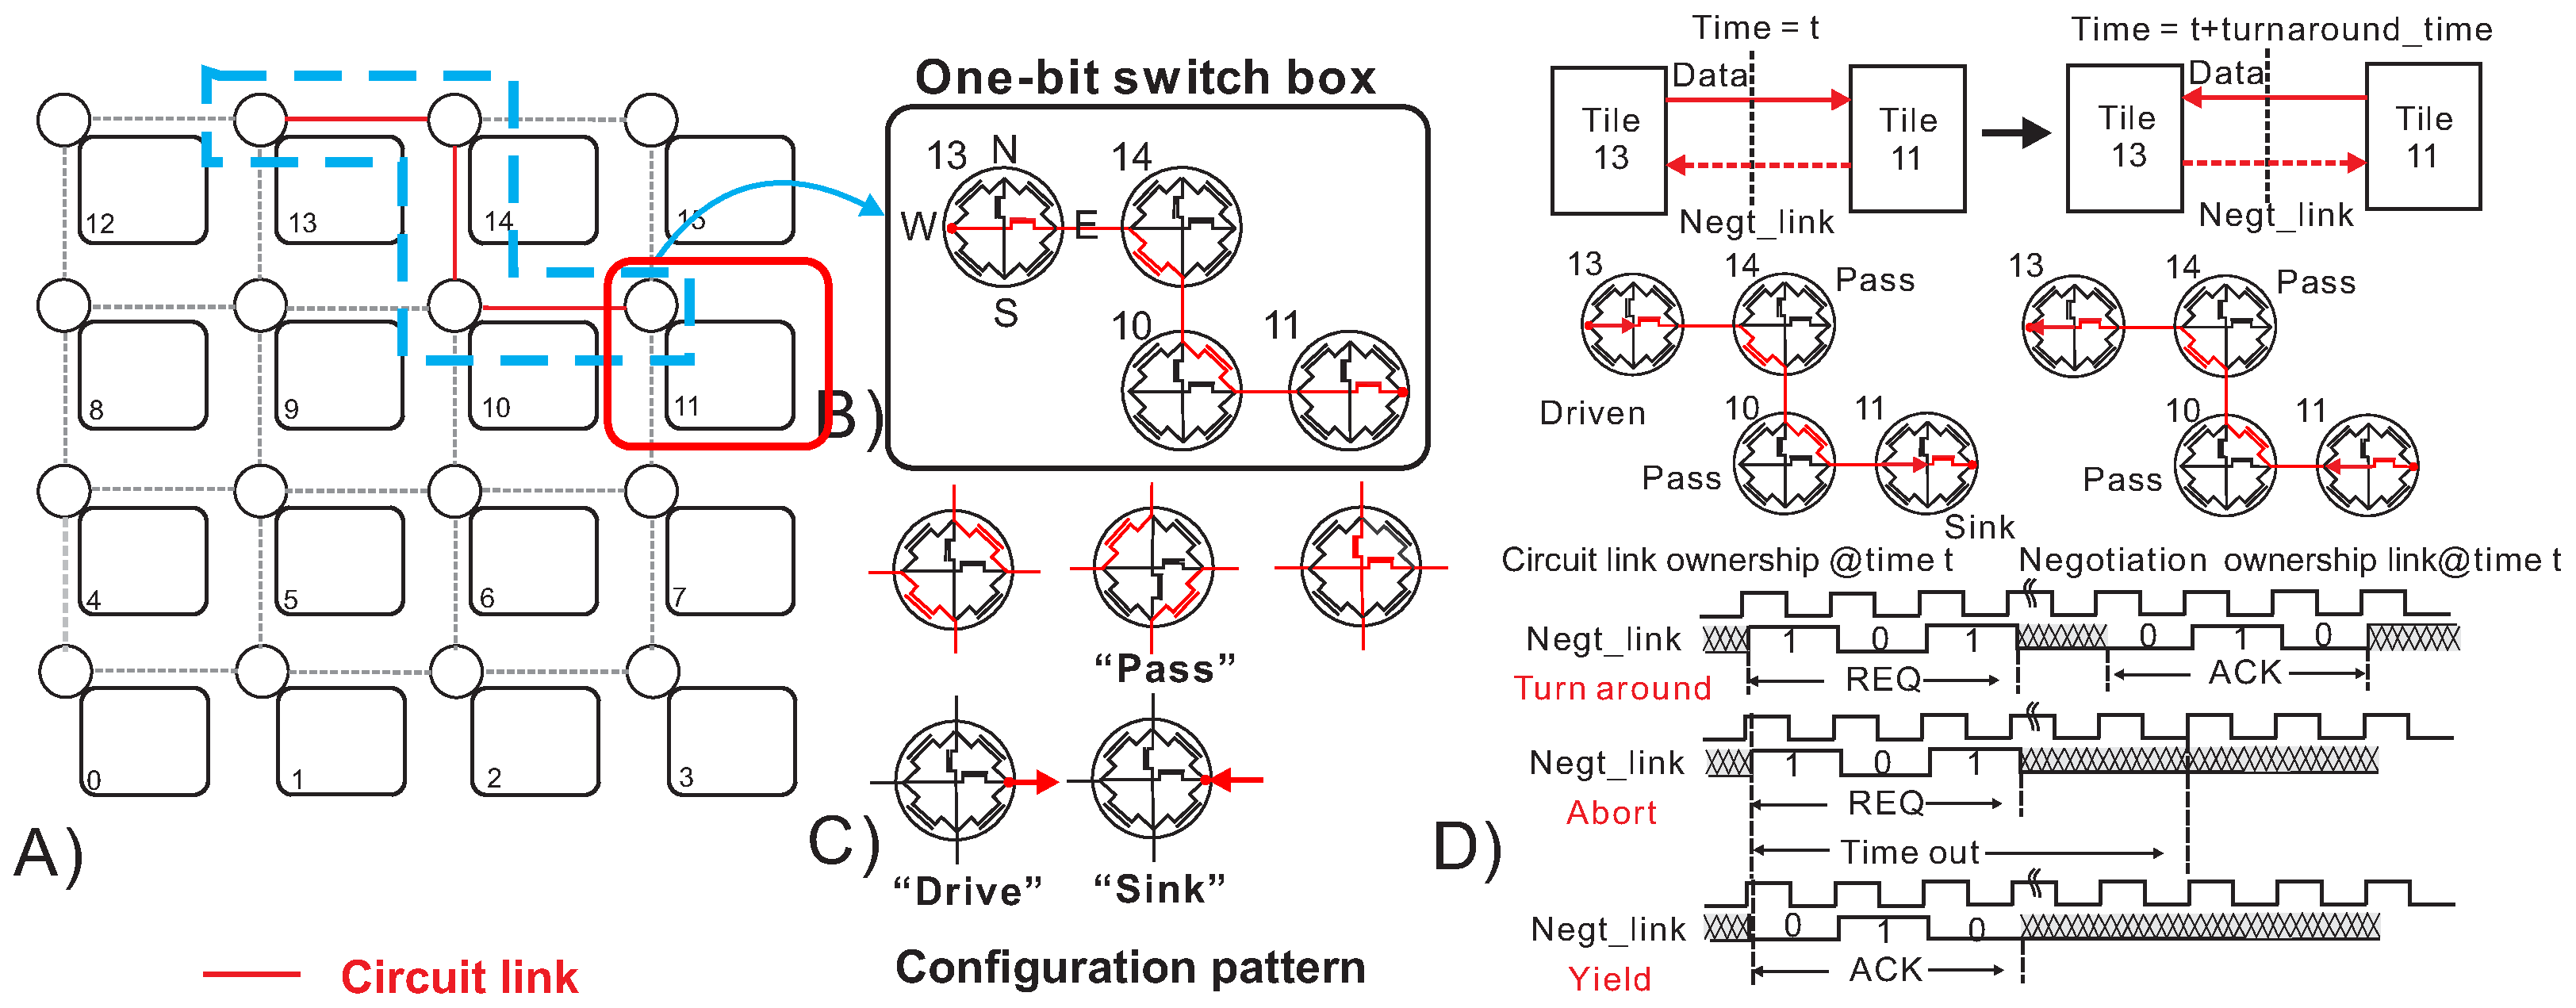
\includegraphics[width=1\columnwidth]{arch_overall.eps}
  \vskip -1mm
  \caption{\textbf{A case study: low-level architecture details} }
  \label{fig:Arch}
  \vskip -7mm
\end{figure}
\begin{algorithm}[t]
\caption{ Greedy maximization algorithm to \eqref{eq:problem_form_2}}
\label{alg:maximization}
\begin{algorithmic}[1]
\REQUIRE ~~\\
    Application  $\mathcal A(t)=(V(t),C(t);\mathcal P(\Sigma,\mathcal F))$; \\
    Reconfigurable NoC $G(t)=(N(t),E(t);\gamma(t),$$\mathcal C)$;\\
    Execution phase length $T$;
    \ENSURE ~~\\
    Compatible application partition $\pi$ and constructed circuit components set $\mathcal T$

\STATE $\pi$=Paritition$(\mathcal A(t),G(t))$
\REPEAT
\STATE $\mathcal T$=$\mathcal T \cup$ $\arg\max\limits_{T_{e}} (\mathcal G(\pi,\mathcal T \cup \mathcal T_e)- \mathcal G(\pi,\mathcal T))$
\UNTIL{$\pi$ is compatible or $\mathcal T==N(t)$}
\end{algorithmic}
\end{algorithm}
%%%%%%%%%%%%%%%%%%%%
\begin{algorithm}[t]
\caption{ $l$-relaxed Greedy maximization algorithm to \eqref{eq:problem_form_2}}
\label{alg:max_2}
\begin{algorithmic}[1]
\REQUIRE ~~\\
    Application  $\mathcal A(t)=(V(t),C(t);\mathcal P(\Sigma,\mathcal F))$; \\
    Reconfigurable NoC $G(t)=(N(t),E(t);\gamma(t),$$\mathcal C)$;\\
    Execution phase length $T$;
    \ENSURE ~~\\
    Compatible application partition $\pi$ and constructed circuit components set $\mathcal T$
\STATE $l=0$    
\STATE $\pi$=Paritition$(\mathcal A(t),G(t))$
\REPEAT
\REPEAT
\STATE $\mathcal T$=$\mathcal T \cup$ $\arg\max\limits_{T_{e}} (\mathcal G(\pi,\mathcal T \cup \mathcal T_e)- \mathcal G(\pi,\mathcal T))$
\UNTIL{$\pi$ is $l$-compatible or $\mathcal T==N(t)$ }
\IF{$\pi$ is $l$-compatible}
\STATE Return $\mathcal T$ and $\pi$
\ENDIF
\STATE $l=l+1$;
\UNTIL{$l== |\arg\max\limits_{\pi_k} |\pi_k||$}
\end{algorithmic}
\end{algorithm}

\section{Architectural Case Study}
%  \begin{figure}[htb]
%  \centering
  % Requires \usepackage{graphicx}
 % \epsfig{file=t_calc.eps}
%  \includegraphics[width=0.85\columnwidth]{negotiation.eps}
%  \caption{\textbf{Self-negotiated link driver/sink turnaround} }
%  \label{fig:negotiated}
%  \vskip -5mm
%\end{figure}
To understand how the proposed mathematical framework could be effectively applied to a reconfigurable NoC system, we consider a simple reconfigurable NoC with switch boxes to provide dedicated links, i.e., the circuit link, between different network tiles. More precisely, we study a regular mesh NoC system $G(t)=(N(t),E(t);\gamma(t))$ to which a subnet of dedicated links is attached. Formally, for each node $n_i \in N(t)$, ACF $\mathcal C$ is induced to generate a set of nodes to which a link could be set up (i.e., ACS, see Definition 5). Therefore, we have a simple reconfigurable NoC system characterized by quadruple $G(t)=(N(t),E(t);\gamma(t), \mathcal C)$. To detail the construction of ACS for each node $n_i$, we set up low-level architectural features for the switch box.

A switch box is a set of programmable pass gates. For simplicity of illustration, Figure \ref{fig:Arch}.(B) shows only the NMOS part of it. To allow circuit links to be set up between different tiles,  a switch box is organized by an array of one-bit switch boxes. The length of the array is equal to the bitwidth of a circuit link. A one-bit swap box consists of 6 pass gates such that any pair of ports can be directly connected by a dedicated link. A tile connects to a switch box through a set of similar links controlled by the pass gates. By cascading such links among a subset of nodes, it is possible to establish circuit links between them.  Figure \ref{fig:Arch}.(B) shows the configuration of a set of switch boxes such that, a set of nodes $\{n_{10},n_{11},n_{13}, n_{14}\}$ becomes a circuit component $\mathcal T_{k}$.

To simplify the hardware setup and minimize the area overhead, we assume each node in the circuit component should time-multiplex the link, i.e., one driver for any circuit link during a slotted time assigned. More precisely, for an execution time of length $T$, each node $n_{i} \in \mathcal T_{k}$ is assigned with a bandwidth, i.e., being a driver for the circuit link, proportional to its traffic share in $q(\mathcal T_{k})$.  Therefore, each switch box could work in 3 possible modes, namely, "Driver", "Sink" and "Pass" based on the ownership of the link. A switch box is in "Pass" mode if the tile connected to the switch is not the driver or sink of the data being transferred, thus "passing" the data. Otherwise, it is in "Driver" or 'Sink' mode. The working modes can be identified by the configuration pattern of switch box as shown in Figure \ref{fig:Arch}.(C). A switch box is in "Pass" mode if \textit{i}) the tile is disconnected to the switch box and \textit{ii}) switch box is programmed as any one of three configurations on top in Figure \ref{fig:Arch}.(C). Otherwise, it will be in "Driver" or "Sink".

As a simple reconfigurable NoC, we enforce the statically assigned time slot for each node in the circuit component. So there is chance that a node becomes the driver yet with no data to transmit. To maximize the link utilization in such case,  it is necessary to make possible the shift of circuit link ownership during such an idle "Driver" phase.  We thus adopt a self-negotiated link access control (SNAC) as shown in Figure \ref{fig:Arch}.(D). We build up a one-bit bi-directional negotiation link (NL) between tiles. A simple negotiation protocol is implemented over the circuit link between a driver-sink pair to bargain over the ownership. More precisely, a "Driver" during its assigned slot will automatically obtain the access to NL and the circuit link. When a data transmission is in progress, no negotiation is necessary. Otherwise, if the driver has no data to send, either a transmission is complete before the expiration of assigned time slot or no planned transmission, driver will send ACK sequence "010" to sink to yield the control over the circuit link to the sink. Upon receiving this sequence, if the sink has anything to send to the current driver, a negotiation happens: the sink will send REQ sequence "101" and wait for ACK sequence. Upon valid ACK, the sink will obtain the rest of time slot and use it for transmission to the previous driver, i.e., the sink and driver switch their roles.  Otherwise, after a preset waiting threshold, the negotiation is a failure and the sink will abort the request. In the following discussion, we will consider a set of real world applications and perform the optimization to construct circuit components by exploiting the submodularity properties of the problem as stated in~\eqref{eq:problem_form_2}.
\section{Experimental Results}
\noindent\textbf{Experiment setup:} We consider real world workloads induced by 6 SoC applications that are characterized by the proposed graphical model $\mathcal A(t)=(V(t),C(t);\mathcal P(\Sigma,\mathcal F))$. The applications include video object plan decoder (VOPD), multi-window display (MWD), MP3 encoder/decoder, H.263 encoder/decoder and MPEG-4. The number of tasks ranges from $11$ to $16$. We set up a 4x4 reconfigurable NoC described in section III as target system. The NoC system is implemented using fully synthesizable Verilog and synthesized under SMIC 65nm process using Synopsys Design Compiler with a fixed frequency constraint of 200MHz. All simulations are done using Synopsys VCS ported with Tcl scripts to load in the application traffic workloads. Throughout the simulations, NoC adopts wormhole switching for regular data transmission under variable flit-width ranging from 16-bit to 256-bit such that,  we can test the network performance under different flit injection rates given a fixed data generation rate. Each port in the router has 4 4-flit virtual channels.  We do not insert repeaters to the circuit links and assume the propagation delay should be within 1 cycle under 200MHz. Thus, we constrain the feasible size of one circuit component to be less than 5. Power estimation is done by feeding the Switching Activity Interchangeable File (SAIF) to Design Compiler during the synthesis.  We extract the switching statistics by RTL simulation in VCS and transform it into SAIF files. Algorithm \ref{alg:max_2} is implemented using C++. We use Fiduccia-Mattheyses algorithm for partition of the applications. 

\noindent\textbf{Performance evaluation:} Figure \ref{fig:task} shows the optimized network configurations for all 6 applications obtained by solving the  submodular maximization problem in (\ref{eq:problem_form_2}). Application partition $\pi$ is first obtained to minimize the cut cost, i.e., traffic between different partition components, see \eqref{eq:problem_form} for detailed explanation. Then, we run the $l$-relaxed greedy maximization algorithm to construct circuit components $\mathcal T$ such that a circuit component configuration is obtained, which is compatible with the partition $\pi$. As shown in Figure \ref{fig:task}, our algorithm identifies the critical traffic paths of all applications (see solid rectangles) and constructs circuit components (dashed rectangles) to cover most of them. An important observation is that the configuration of the network varies greatly for different applications, which suggests the spatio-temporal variability of the applications when ported to the NoC system over time. 
%We first show in Figure \ref{fig:task} the partition $\pi$ for all 6 applications and their corresponding compatible circuit components construction. To obtain feasible partitions under the physical limitations, i.e., propagation delay should be less than 1 cycle, we set the $|\pi_k| \leq 5$ for any partition component, or equivalently for any circuit component.
\begin{figure}[htb]
  \centering
  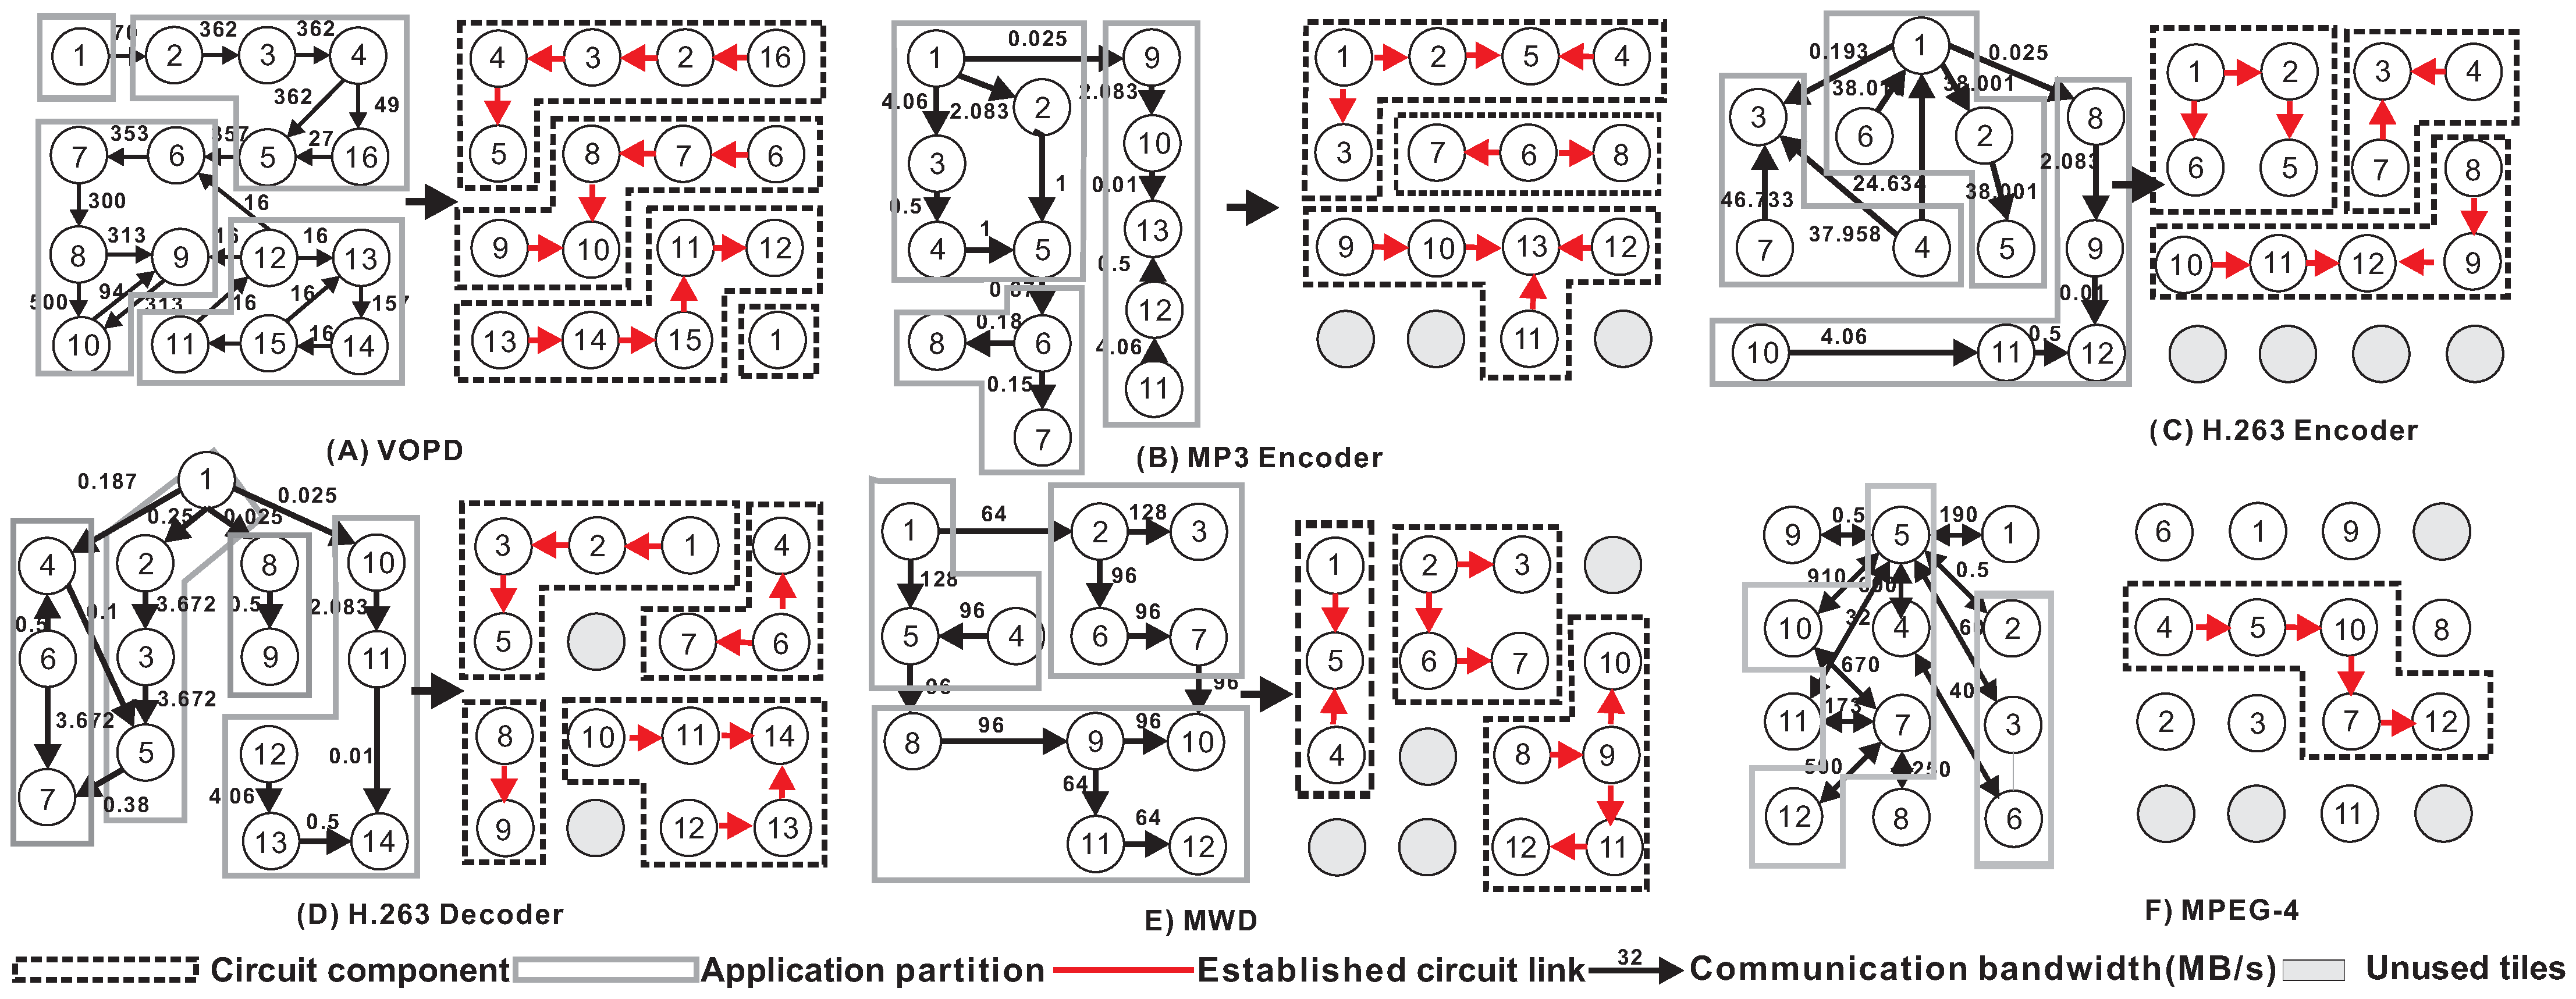
\includegraphics[width=1\columnwidth]{task_3.eps}
  \caption{\textbf{Optimized network configuration for real world applications} }
  \label{fig:task}
  \vskip -4mm
\end{figure}
\begin{figure}[htb]
  \centering
  % Requires \usepackage{graphicx}
 % \epsfig{file=t_calc.eps}
  \includegraphics[width=1\columnwidth]{main_result.eps}
  \vskip -2mm
  \caption{\textbf{Network latency and energy savings comparison between the baseline and optimized reconfigurable NoC under different traffic workloads.(a) Network latency measurements and (b) corresponding normalized energy consumptions. }}
  \label{fig:network}
  \vskip -6.5mm
\end{figure}
\indent To evaluate the performance under different traffic pressures, we run the applications on networks with different physical interconnection bandwidth (i.e., flitwidth=16-bit to 256-bit) under 200MHz to measure the network latency. In such settings, the flit injection rate has to be increased/decreased to meet the application bandwidth requirements as the physical bandwidth shrinks/grows. We compare the network latency for reconfigurable NoC optimized by Algorithm \ref{alg:max_2} and the baseline regular mesh NoC. The results are reported in Figure \ref{fig:network}.(a). For applications with smaller bandwidth requirements like MP3 Encoder, H263 Decoder and Encoder, both networks demonstrate no saturation phase transition under experimental settings. However, the optimized reconfigurable network shows on average $52.3\%$ latency reduction compared to the baseline design. This is because most of the communication with heavy traffic loads are identified and take advantage of the dedicated links without traveling through multiple routing stages.  For applications with heavy traffic requirements like VOPD, MPEG4 and MWD, the optimized network not only shows improved network latency before phase transition, but also exhibits its capability to endure greater traffic pressure, i.e., the network becomes heavily congested under a greater flit injection rate compared to the baseline design. This improvement comes from the fact that, the communication paths with heaviest traffic are covered mostly by the circuit links, thus alleviating the traffic pressure posed on the regular network.

 To show the improved energy efficiency of our optimized network, we report the normalized energy savings under different network settings in Figure \ref{fig:network}.(b). Combined with Figure \ref{fig:network}.(a), we have the following key observations: \textit{i}) Our optimized network shows improved energy efficiency ranging from $22\%$ to $38\%$ with an average of $30.2\%$, under all workloads and \textit{ii}) The energy efficiency increases as the network becomes more congested. These observations are supported by the fact that the traffic over the circuit links consumes less energy by skipping multiple routers. The energy savings are even greater when the network is congested as the recursive switching within a router for blocked packets can be avoided.
\section{Summary}
In this work, we lay the theoretical foundation for modeling the reconfigurable NoC in general and propose a mathematical framework for optimization of the NoC reconfiguration. We formulate the NoC reconfiguration as an optimization problem and prove its submodularity. Based on our theoretical analysis, we propose a greedy algorithm bounded by guaranteed optimality. As a case study, we propose a simple reconfigurable NoC as architectural instance to validate the framework. We perform the proposed optimization and evaluate it with real-world workloads. The results show a $52.3\%$ reduction of network latency on average, increased capability of handling heavy traffic and $30.2\%$ in energy reduction compared to baseline design. 


% More Research Topics
% \include{ResearchTopic2}

% Conclusion and ongoing work
%\chapter{Conclusion and ongoing work}
\label{cha:conclusion}

\Blindtext[2]


\begin{singlespace}
  % Bibliography
  \references{plain}{reference}

  %\appendix
  % Appendices
  %\chapter{A Long Proof}
\label{app:long_proof}

A long proof that nobody is gonna read goes here.

\end{singlespace}

% In case your dissertation has multiple volumes.
% \addvolumecontents{thesis_part2}
% \addvolumecontents{thesis_part3}
% \addvolumecontents[lof]{thesis_part2}

\end{document}
